
%title
%page1

\documentclass[a4paper,20pt]{report}


\usepackage{geometry}
%\usepackage[a4paper, total={6in, 8in}]{geometry}

\geometry{
 a4paper,
 total={170mm,257mm},
 left=20mm,
 top=20mm,
}

%\documentclass{article}
%\usepackage{iftex}
%\iftutex
%% For LuaTeX or XeTeX Use Google's 
%% OpenType Noto fonts for typesetting
%% Russian text
%\usepackage{fontspec}
%\defaultfontfeatures{Ligatures={TeX}}
%%\setmainfont{Noto Serif}
%%\setsansfont{Noto Sans}
%%\setmonofont{Noto Sans Mono}
%\else
%% For pdfTeX we must use old
%% 8-bit font technologies
%\usepackage[T2A]{fontenc}
%\fi
%Hyphenation rules
%\usepackage{hyphenat}
%\hyphenation{ма-те-ма-ти-ка вос-ста-нав-ли-вать}
\usepackage[english, russian, ukrainian]{babel}
\usepackage{csquotes}
\usepackage{xfrac}

\usepackage{fontspec}
\setmainfont{FreeSerif}
\setsansfont{FreeSans}
\setmonofont{FreeMono}

\usepackage{polyglossia}
\usepackage{hyperref}

%\setdefaultlanguage{russian}
\setdefaultlanguage{ukrainian}

%\setotherlanguages{ukrainian}
\setotherlanguages{russian}

%\babelprovide[import]{thai}
\babelfont{rm}{FreeSerif}
\babelfont{sf}{FreeSans}
\babelfont{tt}{FreeMono}

\newif\ifrus
\newif\ifukr
\newif\ifpages

\ukrtrue
\pagestrue



\begin{document}

%\includegraphics[width=\pagewidth]{azov_more_a4.jpg}
\includepdf[pages={1}]{azov_more_title_a4.pdf}
\clearpage

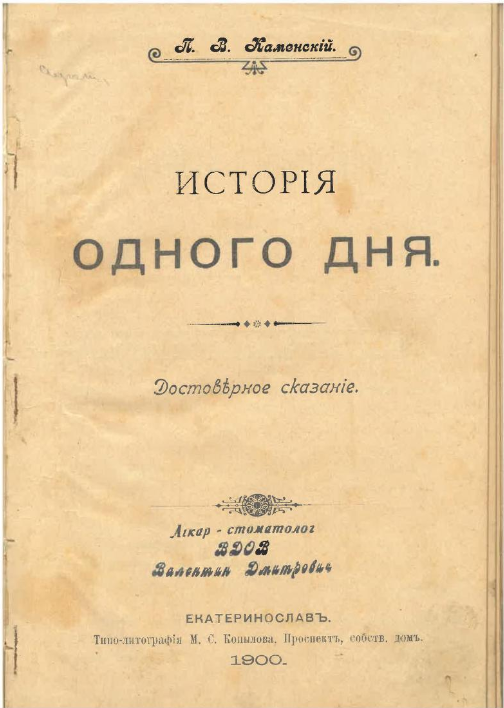
\includegraphics[width=\textwidth]{istoria_odnogo_dnja_title_scan.png}
\clearpage

\begin{quote}
\em

П. В. Каменський

Історія Одного Дня

Достовірна Розповідь

Лікар-Стоматолог ВДОВ

Валентин Дмитрович

Єкатеринослав

Типо-літографія М. С. Копилова. Проспект, власний будинок

1900
%page2
Дозволено цензурою. Харьков, 25 сентября 1900 г.

\end{quote}

%page3
%\ifpages\section{Сторінка 3}\else\fi
\begin{center}
\bfseries\em\Huge
Історія Одного Дня 

(Достовірна Розповідь)
\end{center}

\Large

Біля 20-х чисел березня 1868 року у місті Бердянську, у готелі \emph{``Білий Лебідь''}
орехівський третьої гільдії купець Поддубня, який торгував чаєм, дьогтем та
салом, розповідав двум своїм знайомим, Мазіну та Колосовському, про зловісні
пригоди, які стались із ним у місті Маріуполь. Серед слухачів був також третій
чоловік, невідомий Поддубні, що також слухав розповідь; його звали \textbf{\em
Григорій Власов Ільяшенко}. Він був молодий чоловік років 33, блондин,
зовнішньо нічим особливо собою не помітний, і ніяких, як мовиться у паспортах,
особливих прикмет не мавший.  Родом він був із міста Миколаїв: у час коли
трапилась ця історія він жив разов із своєю жінкою в місті Бердянськ, де
займався приватним чином креслярськими роботами у місцевого архітектора. До
того як він прибув у Бердянськ Ільяшенко знаходився на службі в
севастопольській інженерній команді морської будівельної частини як кресляр та
був нагороджений, як це було підтверджено офіційними документами, бронзовою
медаллю на Андріївскій ленті.

Розповідь Поддубні не була зв'язною. Він почав із пояснення, у чому полягало у
місті Маріуполь особливе грецьке управління, але його пояснення були мало
зрозумілі, бо вони зводились до повторення одних і тих же слів: каторжні
грецькі порядки, прокляте грецьке царство тощо. Зрозуміло, що ці повторювані
фрази, які переплітались із лайкою, ніяк не знайомили із установами, яким
підпорядковувалось у той час грецьке населення. Насправді, ознайомлення із цими
установами не є складною справою.

Переселені в кінці минулого століття із Кримського півострова греки заснували
місто Маріуполь і 23 грецьких села. По пізнішим законодавчим актам они складали
особливий грецький округ, і греки які його населяли підпорядковувались
винятково створеній для них установі, яка називалась грецьким судом. Це була
установа одночасно судова, адміністративна і поліцейська. Його компетенція
розповсюджувалась тільки на греків, а інші національності у компетенцію цього
суду не входили. Суд складався із голови, і трьох членів, які називались
засідателями, секретаря і підпорядкованих йому столоначальників. Всі справи
вирішувались колегіально, і тільки згідно звичаю, але не по закону;
практикувалось, що на одного засідателя покладались поліцейські обов'язки, на
іншого обов'язки слідчого, а третій був відповідальний за господарську частину.
Виключаючи секретаря і підпорядкованих йому столоначальників, решта складу суду
вибирався грецькими поселенцями на трьохлітній період. Для цього один раз у
трьохлітній період кожне із 23-х грецьких поселень надсилало у місто Маріуполь
двух уповноважених, які, разом із представниками міста, вибирали частину складу
грецького суду, тобто голову і трьох засідателей. Згідно звичаю, прийнявшому
внаслідок своєї незмінної повторності силу закону, вибирався завжди той
кандидат, який ставив виборцям більше вина.
%page5
Так як у склад суду потрапляли більшою мірою люди, які не тільки не мали адміністративного та суддівського досвіду,
але які були недостатньо освічені, поняття яких не йшли далі питань про \emph{``паляницю та льон''}, то, для навернення
їх на шлях законності та відповідного усвідомлення цих шляхів, влада призначала та надсилала із губернського міста 
Єкатеринослава спеціально до цього призначеного секретаря, який ще називався стряпчим та який мав відповідні
прокурорські права.
%Так как в состав суда попадали большей частью люди, не только не блиставшие административным и судебным опытом,
%но даже недостаточно грамотные, понятия которых не шли дальше вопросов о ``паленице и льне'', то,
%для наставления их на путь законности и достодолжного уразумения сих путей, правительством назначался
%и присылался из губернского города Екатеринослава нарочито к сему приспособленный секретарь, именовавшийся
%еще стряпчим и обладавший прокурорскими правами.

Із подальшої розмови, що відбулася між відвідувачами готелю \emph{``Білий Лебідь''}, можна було
дізнатись, що в кінці 50-х і на початку 60-х років членом грецького суду був якийсь
житель міста Маріуполь \textbf{\em Логафетов}; він відповідав за поліцейську частину, і був,
таким чином, адміністратором, в обов'язки якого входила задача поліпшення стану маріупольського
грецького округу та його жителів.
%Из дальнейшего разговора, происходившего между посетителями гостиницы ``Белого
%Лебедя'', можно было узнать, что в конце 50-х и начале 60-х годов членом
%греческого суда состоял некий обыватель гор. Мариуполя, Логафетов; он ведал
%полицейскую часть, был, таким образом, администратором, имевшим своей задачей
%споспешествовать благоустроению мариупольского греческого округа и его
%обывателей. 
В цій своїй ролі він не залишив нічого пам'ятного своїм нащадкам. Але як поліцейський чин,
який керував обходами під час ярмарок у Маріуполі, Логафетов став широко відомим; 
чутки пов'язували його ім'я із цілим рядом невеликих та більш суттєвих злочинів.
%В этакой своей роли он ничего памятного потомству не оставил. Но за
%то, как полицейский чин, руководивший обходами во время ярмарок в Мариуполе,
%Логафетов приобрел широкую известность; молва соединяла его имя с целым рядом
%мелких и крупных преступлений. 
Славнозвісні логафетовські обходи, які надовго збереглися у пам'яті нащадків, зазвичай полягали
у наступному: під своїм керівництвом Логафетов збирав загін із сторожів грецького суду і тих молодих
людей із міста, які під час ярмарок приходили в його загін у якості волонтерів. Із таким от загонов 
Логафетов і відправлявся на ярмарок ``наглядати за порядком''. Але насправді вся ця банда віддавалась
розпусті, гульбощам та обжерливості, але що було добре, у ярмарочних шинках та трактирах цих охоронителів
порядку безоплатно годували та поїли, пам'ятаючи про
%Знаменитые логафетовские обходы, надолго
%сохранившиеся в памяти потомства, обычно состояли в следующем: под своим
%начальством Логафетов составлял отряд из сторожей греческого суда и тех молодых
%людей из города, которые во время ярмарок поступали в его отряд в качестве
%волонтеров. С таким отрядом, заседатель греческого суда Логафетов отправлялся
%на ярмарку ``смотреть за порядком''. На самом же деле вся эта банда предавалась
%разврату, кутежам и обжорству, благо, в ярмарочных кабаках и трактирах этих
%охранителей порядка безвозмездно кормили и поили, в виду
%page6
їх значення як начальників. Але шукати розправи і суда шукати було ніде, по дальності відстані
від високого начальства, губернатора і по безплодності результатів розслідувань, які виконувались
надсилаємими чиновниками-ревізорами.
%их начальственного значения. Расправы же и суда искать
%было негде, по дальности расстояния от высшего начальства, губернатора и по безплодности
%результатов расследований, производимых присылавшимися чиновниками-ревизорами.
Одного разу, під час такого начальствованія на ярмарку із своїм обходом, Логафетов
зустрів козака Капсуленко, який різко відповів на вимогу не курити. Відбулась свалка; 
Капсуленко впав, отримавши смертельну рану у бік, яка була нанесена йому дротиком, який
Логафетов носив замість палки. Хоча смертельний удар і не був нанесений особисто
Логафетовим, але одним із його поплічників, тим не менш, у місті Маріуполь усі передавали
за достовірне, що засідатель - вбивця козака, що розслідування по справі про цей злочин
не дало ніяких результатів, внаслідок того, що Логафетов встиг схилити людей свого обходу до дачі
брехливих свідчень, які його обілили. Чутки вказували на виверткість Логафетова перед старою слідчою
владою та додавали, що Бог покарав деяких нечестивих, які брехливо свідчили після присяги; запевняли, що
лжесвідки були уражені раптовою смертю зараз, після дачі хибних свідчень. 
%Однажды, во время такого начальствования на ярмарке со своим обходом, Логафетов повстречал казака
%Капсуленко, который резко ответил на требование не курить.
%Произошла свалка; Капсуленко пал, получив смертельную рану в бок, нанесенную ему дротиком,
%который Логафетов носил вместо палки. Хотя смертельный удар и не был нанесен лично
%Логафетовым, а одним из его споспешников, тем не менее, в гор. Мариуполе
%все передавали за достоверное, что заседатель - убийца казака
%расследование по делу об этом преступлении не дало никаких результатов, вследствие того, что
%Логафетов успел склонить людей своего обхода к даче ложных показаний, которыми его обелили.
%Молва указывала на изворотливость Логафетова перед старой следственной властью и добавляла, что Бог
%покарал некоторых нечестивцев, лжесвидетельствовавших после присяги: уверяли, будто
%лжесвидетели были поражены внезапной смертью сейчас,
%после дачи ложных показаний.
Про всі ці викладені обставини Поддубня розповідав своїм слухачам. Одночасно
передав він і їм і те, що особисто над ним проробив Логафетов у 1861 році. ``\emph{Приїхав
я, значить, із товаром на ярмарок''.} - каже Поддубня, - \emph{``розторгувався на перший сорт, спустив усякого
товару. Отримав чистоганом на гроші 5,015 рублів, сховав гроші під жилетку і, звичайно, напився п'яним, почав 
вимагати музику''.}..
%Обо всех этих изложенных обстоятельствах рассказывал Поддубня своим слушателям. 
%Одновременно передал он и им и то, что лично над ним проделал Логафетов в 1861 году.
%``Приехал я, значит, с товаром на ярмарку. - 
%говорит Поддубня, — расторговался на первый сорт,
%спустил всякого товару. Выручил чистоганом на деньги
%5,015 рублей, запрятал деньги под жилетку и, конечно,
%напился пьян, потребовал музыку''...

%page7
Коли в забрудненому сміттям ярмарковому трактирі три обірваних музиканта, які
були озброєні двума інструментами, які були схожі на скрипки та бубном, тішили
слух п'яного Поддубні, у іншому кутку того же трактиру, Логафетов із своїм
загоном віддавався даровому обжерству та пияцтву. Затуманілий надмірної
кількістю їжі та надмірно випитим, Логафетов почав бешкетувати та вимагати,
щоби музику, яка тішила Поддубню, негайно почали би грати перед ним. І як би не
був п'яний Поддубня, але він виступив захисником своїх прав, кажучи, що він
заплатив за музику наперед, і що він не відпустить, \emph{``аж поки вона не відіграє
свого''.}

%Когда в загрязненном сором ярмарочном трактире три оборванных музыканта,
%вооруженных двумя иструментами, похожими на скрипки и бубном, услаждали пьяный
%слух пьяного Поддубни, в другом углу того же трактира, Логафетов со своим
%отрядом предавался даровому обжорству и пьянству. Отуманенный чрезмёрной едой и
%излишне выпитым, Логафетов стал буйствовать и потребовал, чтобы музыка,
%услаждавшая Поддубню, немедленно стала бы играть перед ним. Как ни был бы пьян
%Поддубня, но он выступил защитником своих прав, говоря, что он музыке заплатил
%вперед, и что он не отпустит, ``пока она не отыграет своего''.

Виникло непорозуміння, в результаті якого Поддубня виявився викинутим із
зав'язаними назад руками у якийсь напівтемний чулан, названий арестантською
камерою. Тут Поддубня заснув міцним п'яним сном, від якого прокинувся годин
через п'ять, коли якийсь невідомий чоловік почав виштовхувати його на свободу.
Жах охопив в'язня, коли він, намацавши у себе під жилетом, виявив відсутність
грошей. Він одразу протверезів і зрозумів, що в кінец є розорений, оскільки там
під жилетом знаходилась виручка за увесь повністю проданий товар, він тепер
зрозумів, що тепер не було вже ні товару ні грошей. Залишилась злиденність.
Поддубня звернувся за допомогою до місцевої влади, але це виявилось марним.
\emph{``Там прокляте грецьке царство''} - пояснював він своїм слухачам, - \emph{``Логафетов
багатий, у нього велика рідня, знайомства, наш брат тут нічого не вдіє''}...
Писав Поддубня скаргу і губернатору, що визвало розслідування особо
командированого чиновника, який, списавши багато паперу, так і не прийшов ні до
якого результату. Загалом же скарги на Логафетова Поддубні та інших осіб,
%page8
%Произошло недоразумение, в результате которого Поддубня оказался выброшенным с
%завязанными назад руками в какой-то полутемный чулан, названный арестантской
%камерой.  Здесь Поддубня заснул крепким пьяным сном, от которого очнулся часов
%чрез пять, когда какой-то неизвестный человек стал выталкивать его на свободу.
%Ужас охватил узника, когда он, ощупав у себя под жилетом, заметил отсутствие
%денег. Он сразу отрезвел и понял, что в конец разорен, так как там под жилетом
%находилась выручка за весь полностью проданный товар, он понял, что теперь не
%было ни товара, ни денег. Осталась нищета. Поддубня обратился за помощью к
%местным властям, но это оказалось бесполезным. ``Там проклятое греческое
%царство'' - объяснил он своим слушателям, - ``Логафетов богат, у него большая
%родня, знакомства, наш брат ничего не поделает''...  Писал Поддубня жалобу и
%губернатору, что вызвало расследование особо командированного чиновника,
%который, исписав много бумаги, ни к какому результату не пришел. В общем же
%жалобы на Логафетова Поддубни и других лиц, вызвали
призвели його до усунення обов'язків члена грецького суда. Від цього, звісно,
не було легше Поддубні: гроші його пропали. \emph{``По світу спустив, проклятий...
грабіжник''} ... - закінчив свою розповідь Поддубня, прикрасивши своє заключне
слово тією багатою по своїм відтінкам лайкою, яка не допускається в печаті,
хоча й тепер її нерідко можна почути на вулицях у великих навіть містах. Коли
Поддубня закінчив, Ільяшенко втрутився у розмову. Він запропонував Поддубні
\emph{``узятись''} за його справу і пояснив, що раніше з успіхов вів перед начальством
справи молокан. І дійсно, безперечними офіціальними даними встановлено, що
Ільяшенко  відвідував колонії молокан, оглядав їх на манер ревізора-чиновника,
виражав їм іноді своє благовоління, похвали і обіцянки про клопотання перед
високим начальством у Петербурзі, якого, звісно, він ніколи не виконував і
виконати не міг. При цьому варто зауважити, що Ільяшенко у цьому випадку діяв
\emph{``без усілякої користолюбної цілі і навіть без особливої спонукальної
причини''}.  (Див. в архіві єкатеринославского окружного суда: журнал рішень за
1965 р. л. 29 л. д. 14 об).

%page8
%устранение его от исполнения обязанностей члена греческого суда. От этого,
%конечно, не было легче Поддубне: деньги его пропали. ``По миру пустил,
%проклятый... грабитель'' ... - заключил свой рассказ Поддубня, уснастив свое
%заключительное слово теми богатыми по своим оттенкам ругательствами, которые,
%(хотя еще и теперь нередко слышатся на улицах в больших даже городах) нетерпимы
%в печати.  Когда Поддубня кончил, Ильяшенко вмешался в разговор. Он предложил
%Поддубне ``взяться'' за его дело и пояснил, что раньше с успехом вел пред
%начальством дела молокан.  Действительно, безспорными официальными данными
%устанавливается, что Ильяшенко посещал колонии молокан, осматривал их на манер
%ревизора-чиновника, выражал им иногда свое благоволение, похвалы и обещания
%предстательства пред высшим начальством в Петербурге, какового, конечно, он
%никогда не исполнял и исполнять не мог. При
%этом достойно замечания, что Ильяшенко в этом случае действовал ``без всякой
%корыстной цели и даже без особой побудительной причины''. (См. в архиве
%екатеринославского окружного суда: журнал решений за 1965 г. л. 29 л. д. 14
%об).
На пропозицію Ільяшенко узятись за справу, Поддубня відповів відмовою, зауваживши...
``із чем же вести справу, коли я залишився голим як сокіл!'' ``ну так знайте'', заперечив Ільяшенко,
``я вам цього самого Логафетова у кандалах через Бердянськ відправлю у єкатеринославську тюрьму!''
До сих пір розмова відбувалась відносно спокійно і на ви, але, після слів, сказаних Ільяшенко, Поддубня 
впав у патетичний тон і перейшов на ти:
``будь благодійником, замкни його у тюрьму, останню сорочку зніму, віддам!'' ... закричав Поддубня. ``Нічого не треба,
тільки поставиш могорич'', удавав із себе великодушного Ільяшенко,
%На предложение Ильяшенко взяться за дело, Поддубня ответил отказов, заметив...
%``с чем же вести дело, когда я остался гол как сокол!'' ``ну так знайте'', возразил Ильяшенко, ``я вам этого самого 
%Логафетова в кандалах чрез Бердянск отправлю в екатеринославскую тюрьму!''
%До сих пор разговор происходил сравнительно
%спокойно и на вы, но, после слов, сказанных Ильяшенко,
%Поддубня впал в патетический тон и перешел на ты:
%``будь благодетель, запри его в тюрьму, последнюю сорочку сниму, отдам!''... завопил Поддубня. ``Ничего не надо,
%только поставишь могарыч'', великодушничал Ильяшенко, 
%page9
після чого раптово познайомлені обійняли один одного, і стали пити воду із знову принесеної пляшки. Біля цього
сосуду об'єдналась уся компанія із чотирьох чоловік, і дружньо вела голосним шопотом якусь довгу розмову.
%после чего внезапно познакомившиеся заключили друг друга в объятия, 
%и стали пить воду из вновь принесенной бутылки. Возле этого сосуда объединилась вся компания из
%четырех человек, и дружно вела громким шопотом какой-то длинный разговор.
День 5 квітня 1863 року був одним із тих весняних днів, коли зима робить
останню вилазку супроти наступаючого літа. Було ``сиверко'', як каже наш
простий народ; небо заволокло сірими хмарами, які не міг прогнати пронизаючий,
ні на одну хвилину не ослаблюючий своєї поривчастості північно-східний вітер;
степ не встиг ще покритись зеленню, і разом із сірим небом, представляв собою
як би суцільну сіровато-буру масу. Якщо би не довгі дні, та не особливе весняне
освітлення, яке, не дивлячись на хмари, що затулили сонце, таки відчувалось, то
можна було би подумати, що пори Роки повернули назад, що наступив листопад
місяць. Ледве з'явившийся ``накат'' по дорогам зіпсувався, завдяки дощу, що
безупинно падав на землю. Посеред такої обстановки, у вказаний день 5 квітня,
по дорозі із Бердянська в Маріуполь, верстах у двадцяти під останнього міста,
їхала однокінна підвода, на якій сиділи вже відомі нам особи: купець Мазин,
міщанин Колосовський та відставний кресляр Григорій Власов Ільяшенко. (Див. в
архіві єкатеринославського окружного суда справу, що вступила в палату із
олександрівського повітового суда разом із міскою ратушею про відставного
кресляра із обер-офіцерських дітей Гр. Вл. Ільяшенко л. д. 12).
%День 5 апреля 1863 года являлся одним из тех весенних дней, когда зима делает
%последнюю вылазку против наступающего лета.  Было ``сиверко'', как говорит наш
%простой народ; небо заволокло серыми тучами, которых не мог прогнать
%пронизывающий, ни на одну минуту не ослаблявший своей порывистости
%северо-восточный ветер; степь не успела еще покрыться зеленью, и вместе с серым
%небом, представляла как бы сплошную серовато-бурую массу. Если бы не длинные
%дни, да не особое весеннее освещение, которое, несмотря на закрывшие солнце
%тучи, таки ощущалось, можно было бы подумать, что времена Года повернули
%вспять, что настал ноябрь месяц. Едва образовавшийся ``накат'' по дорогам
%испортился, благодаря безпрерывно сыпавшемуся на землю мелкому дождю.  Среди
%такой обстановки, в указанный день 5 апреля, по дороге из Бердянска в
%Мариуполь, верстах в двадцати от последнего города, тащилась одноконная
%подвода, на которой сидели уже известные нам лица: купець Мазин, мещанин
%Колосовский и отставной чертежник Григорий Власов Ильяшенко. (См. в архиве
%екатеринославского окружного суда дело, вступившее в палату из александровского
%уездного суда обще с городовой ратушей об отставном чертежнике из
%обер-офицерских детей Гр. Вл. Ильяшенко л. д. 12).
Вони їхали більш ніж 50 верст по невеселій дорозі; їм залишалось до Маріуполя
ще верст 25 такого ж невеселого шляху.  Перед подорожуючими простирався ще той
же степ - однорідний, сірий, без деревця, без будь якого пейзажу, на якому можна було б зупинити око.
%Верст более 50 по невеселой дороге ехали они; им оставалось до Мариуполя еще верст 25 такого же невеселого пути. 
%Пред путниками простиралась все та же степь
%однородная, серая, без деревца, без какого то ни было пейзажа, на котором можно
%остановить глаз. Но наши путешественники относились к этому равнодушно и сидели
%page10
Але наші мандрівники відносились до цього байдуже і сиділи на своїй жалюгідній
повозці, бувши в тій апатії, що оволодіває мандрівником, добре наперед знаючим,
що ніякими зусиллями, хитрощами, благаннями не скоротити і не
змінити довгих виснажуючих годин шляху посеред мовчазного степу.
%на своей невзрачной повозке, проникнутые той апатией, которая по необходимости
%овладевает путником, хорошо наперед знающим, что никакими усилями, хитростями,
%мольбами, едущему не сократить, ни изменить долгих томительных часов пути среди
%безмолвных степей.
Біля чотирьох годин після полудня Ільяшенко та його товариші під'їхали до Маріуполя
і зупинились у передмісті міста, на Маріїнській стороні, в одній із непомітних хатинок;
готелів тоді у Маріуполі не було і приїзджаючі зупинялись у приватних квартирах. Того ж дня ввечері,
коли вже стемніло, Ільяшенко розшукав будинок Логафетова і приїхав до цього останнього.
(журнал рішення єкатеринославської палати уголовного суду за 1865 р., л. 29). Як ми вже знаємо, 
Логафетов у той час не був владою: він був усунений від посади члена грецького суда. Тим не менш він
жив у своє задоволення: був холостий, багатий, не особливо старий, йому було десь 50 років, хворобами
не страждав, у місті мав багатих та сильних родичів, серед яких він був свій та дорогий їх серцю чоловік.
Словом жилось йому добре, безтурботно, спокійно; його службові подвиги його не тривожили, бо ж усі розслідування
про його минулі діяння скінчились зовсім щасливо: ні про які судове переслідування не було й мови. Ось чому Логафетов
зверхньо віднісся до Ільяшенко, коли той став йому пояснювати, що йому загрожують неприємності
по скаргам Поддубні, і коли Ільяшенко запропонував йому свою допомогу для владнання цієї справи. В кінці кінців
Логафетов грубо вирядив Ільяшенко та закриваючи за ним двері, пропустив повз вуха звернений до нього
вигук: ``ти мене ще згадаєш!''... Зрозуміло, що цим словам Логафетов не надав рівно ніякого значення.
%Около четырех часов пополудни Ильяшенко и его товарищи подъехали к Мариуполю и
%остановились в предместьи города, на Марьинской стороне, в одной из невзрачных
%изб; гостиниц тогда в Мариуполе не было и приезжающие останавливались в
%частных квартирах. Того же дня вечером, когда уже стемнело, Ильяшенко разыскал
%дом Логафетова и явился к этому последнему.
%(журнал решения екатеринославской палаты уголовного суда за 1865 г., л. 29). Как мы уже знаем, Логафетов в
%то время не был властью: он был устранен от должности члена греческого суда. Тем не менее он жил
%припеваючи: был холост, богат, не особенно стар, ему
%было около 50 лет, недугами не страдал, в городе имел
%богатых и сильных родственников, среди которых он
%был свой и дорогой их сердцу человек. Словом жилось
%ему хорошо, беззаботно, спокойно; его служебные подвиги
%ето не тревожили, ибо все расследования о его прошлых деяниях 
%кончились совсем благополучно: ни о каких судебных 
%преследованиях не было и речи. Вот почему Логафетов свысока отнесся к Ильяшенко, когда тот стал
%ему объяснять, что ему грозят неприятности по жалобам
%Поддубни, и когда Ильяшенко предложил ему свое содействие для улаживания этого дела. В конце концов
%Логафетов грубо выпроводил Ильяшенко и закрывая за ним 
%page11
%дверь, пропустил мимо ушей обращенное к нему восклицание: ``ты меня попомнишь!''...
%Понятно, что этим словам Логафетов не придал ровно никакого значения. 

\par\noindent\rule{\textwidth}{0.4pt}

\textbf{\em Mihi non pudet fateri nescire, quod nesciam} і мені не соромно
зізнатись, що у мене немає вміння писати творчо, створюючи художні типи,
частково розкидані у життю. Якщо би я володів таким вмінням, я надав би
перевагу зображенню описаних подій у формі комедії або драми, і в цьому місці
зображення дійсності опустив би завісу, закінчивши I-й акт.

Потім я почав би 2-й і останній акт, таким чином внесши більше інтересу і життя у цю роботу;
але, на жаль, це не під силу мені; я є лише смиренний літописець-протоколіст, і відновлюю забуту і,
на мій погляд повчальну історію по тому способу і прийому, як складають
звичайний судовий або поліцейський протокол. При цьому я використовував безсумнівні документи, що зберігаються
в архіві єкатеринославського окружного суду, дозвіл на переглядання яких був мені люб'язно наданий поважним
головою названого суду І. Ц. Патоном; потім я маю у своєму розпорядженні знайдену моїм шанованим 
товаришем уїздним членом таганрогзського окружного суду В. С. Станкевичем кореспонденцію ``Сина Вітчизни''
за 20 травня 1869 року та передану ними мені; накінець я широко користувався свідчими показаннями деяких старожилів міста Маріуполь,
які були не тільки безпосередніми свідками, але навіть учасниками описуваних мною подій.
%\textbf{\em Mihi non pudet fateri nescire, quod nesciam} и мне не стыдно сознаться, что у
%меня нет умения писать творчески, создавая художественные типы, частично
%разбросанные в жизни.  Если бы я обладал таким умением, я предпочел бы
%изобразить описываемые события в форме комедии или драмы, и в этом месте
%изображения действительности опустил бы занавес, закончив I-й акт.

%Затем я начал бы 2-й и последний акт, так внесено было бы более интереса и жизни в настоящую работу;
%но, к сожалению, это не под силам мне; я только смиренный летописец-протоколист, и восстанавливаю
%забытую и, на мой взгляд поучительную историю по тому способу и приему, как составляют обыкновенный судебный или
%полицейский протокол. При этом я пользовался бесспорными документами, хранящимися в архиве екатеринославского
%окружного суда, просмотр коих любезно был мне предоставлен почтенным председателем
%названного суда И. Ц. Патоном; затем я имею в своем распоряжении разысканную моим уважаемым 
%товарищем уездным членом таганрогского окружного суда В. С. Станкевичем корреспонденцию 
%``Сына Отечества'' от 20 мая 1869 года и переданную ими мне; наконец я широко воспользовался свидетельскими 
%показаниями некоторых старожилов г. Мариуполя, которые были не только непосредственными 
%свидетелями, но даже отчасти участниками описываемых мною событий.
%page12
Користуюсь нагодою приношу мою глибоку вдячність цим старожилам, із яких
деякі не побажали, щоби я згадував їх імена; я їм дякую за їх довгі, детальні свідчення та головним чином
за вражаючу вірність та точність їх свідчень, у чому я переконався співставлюючи їх покази
документальними даними, які зберігаються в архіві єкатеринославскього окружного суду. Після цього пояснення
продовжую перерваний протокол.
%Пользуюсь случаем принести мою глубокую благодарность этим старожилам, из
%которых некоторые не пожелали, чтобы я упомянул их имена; я их благодарю за их
%длинные, подробные показания и главным образом за поразительную верноеть и
%точность их свидетельств, в чем я убедилея сопоставляя их показания
%документальными данными, хранящимися в архиве екатеринославского окружного
%суда. После этого объяснения продолжаю прерванный протокол.
6 квітня 1863 року писар, що завідував канцелярією 
\textbf{\em ``Начальника Маріупольської команди внутрішньої стражі''}, в
установленому порядку, у 8 годин ранку, з'явився у невелику кімнату, на дверях
якої був прибитий напів-лист паперу із криво виведеним великими літерами
надписом: ``Канцелярія''. Писар був із молодих; цю посаду він займав тільки із
1862 року. Раніш він входив у склад команди, що була сформована у місті
Єкатеринославі із 40 рядових; команда була сформована в 1858 році, і в тому ж
році була надіслана у місто Маріуполь під головуванням її постійного начальника
капітана Лисенко. В команду, про яку йде мова, входили солдати найкращої
репутації, що мали нашивки. По свідченням старожилів у той час панувала
найсуворіша воєнна дисципліна: ``достатньо було чихнути во фронті, щоби
отримати в морду від начальства'', привожу справжні слова одного бувшого
солдата команди. Варто зауважити, що, даючи такі свідчення, старожили із бувших
солдат тим не менш додають: ``жити було прекрасно''. Потім вони пояснюють що
всі знали одне одного, що ``не було крадіжок, грабунків, шахрайства, готелів та
візників не було''. Очевидно, значить, що витівки та злочини Логафетова не йшли
у рахунок: ймовірно, їх ігнорували через повагу до його стану як начальника.
%6 апреля 1863 года писарь, заведывавший канцелярией 
%\textbf{\em ``Начальника Мариупольской команды внутренней стражи''},
%по заведенному порядку, в 8 час. утра, явился в небольшую комнату, на дверях которой был прибит полу-лист
%бумаги с криво выведенною большими буквами надписью: ``Канцелярия''. Писарь был из молодых; эту должность он занимал только с 1862 года.
%Раньше он входил в состав команды, сформированной в г. Екатеринославе из 40 рядовых; команда была сформирована в 1858 году, и в тот же год была прислана в город Мариуполь под начальством ее постоянного начальника капитана Лисенко. 
%В команду, о которой идет речь, входили солдаты лучшей репутации, имевшие нашивки. По свидетельству старожилов
%в то время господствовала строжайшая военная
%дисциплина: ``достаточно было чихнуть во фронте, чтобы
%получить в морду от начальства'', привожу подлинные
%слова одного бывшего солдата команды. Замечательно при
%этом, что, давая такие показанля, старожилы из бывших
%солдат тем не менее добавляют: ``жить было прекрасно''.
%Далее они объясняют что все знали друг друга, что 
%``воровства, грабежа, мошенничества, извозчиков и гостиниц
%не было''. Очевидно, значит, что проделки и преступления Логафетова в счет не шли: вероятно, их
%игнорировали из уважения к его начальственному состоянию.
%page13
Писар військової команди відрізнявся як зразковий ``службіст'' і за зразкове
виконання дисципліни, у 1860 році, був зроблений унтер-офіцером. Обов'язки
писаря він виконував із тою же незмінною старанністю, з тим же строгим
виконанням дисципліни, як і обов'язки рядового.
%Писарь войсковой команды отличался как образцовый ``службист'' и за образцовое
%исполнение дисциплины, в 1860 году, был произведен в унтер-офицеры. Обязанности
%писаря он исполнял с тем же неизменным усердием, с тем же строгим исполнением
%дисциилины, как и обязанности рядового.
Прийшовши 6 квітня у свою канцелярію, писар підійшов до великої, незграбної грубо зробленої косої шафи,
дістав із неї декілька товстих зошитів у потертій палітурці і поклав їх на тут же стоявший великий стіл, такий же 
незграбний як і сама шафа.
%Прийдя 6 апреля в свою канцелярию, писарь подошел к большому, неуклюжему, грубо сделанному,
%косому шкафу, достал из него несколько толстых тетрадей в потертом переплете и положил их на тут же
%стоявший большой стол, такой же неуклюжий, как и шкаф.
Потім, обмакнувши у бульбашку із чорнилом гусине перо, він став цією скрипучою зброєю
виводити букви на сірому, трохи мохнатому і схожому на войлок папері, із якого були зроблені
книги для вхідних та вихідних паперів.
%Затем, обмакнув в пузырек с чернилом гусиное перо, он стал этим скрипучим
%орудием выводить буквы на серой, немного мохнатой и похожей на войлок бумаге,
%из которой состояли книги для входящих и исходящих бумаг.
``У той час'' (так показує бувший писар, який зараз щасливо проживає у місті Маріуполі)
\begin{quote}
\bfseries\em
твердою ходою, не поспішаючи але і не сповільняючись, входить охайний солідний
із бравим виглядом панок років тридцяти; зросту він був вище
середнього, блондін, одягнений у поганеньке пальто світло-коричневого
кольору, помітно потерте; у такі пальто зазвичай наряджені приказчики,
що стоять за прилавком
\end{quote}

%``В то время'' (так показывает бывший писарь, ныне благополучно проживающий в гор. Мариуполе), 
%\begin{quote}
%\bfseries\em
%твердым шагом, не спеша, но и не медля, входит приличный, 
%солидный, с бравым видом господин лет тридцати. Роста он был выше среднего, блондин, одет в плохонькое пальто
%светло коричневого цвета, заметно потертое; в такие пальто обыкновенно наряжены приказчики, стоящие за прилавком
%\end{quote}
Невідомий, увійшовши у канцелярію, привітався із писарем; останній встав,
витягнувся, поклонився, мовчки сів і знову почав старанно виводити букви, але
душа його була вже охоплена якоюсь неясною тривогою.
%Неизвестный, войдя в канцелярию, поздоровался с писарем; последний встал,
%вытянулся, поклонился, молча сел и стал опять усердно выводить буквы, но душа
%его была уже охвачена какой-то неясной тревогой.
Писар відчув, що незвичайна поява невідомого пана є неспроста.
Між невідомим і писарем у цей час зав'язався наступний діалог.

%page14
\textbf{\em Невідомий}: - Хто є начальник?

\textbf{\em Писар}. - Штабс-капітан Лисенко...

\textbf{\em Невідомий.} - Чи добре відноситься до солдат?

\textbf{\em Писар.} - Так точно, все є добре, дозвольте доповісти начальн...

\textbf{\em Невідомий} (різко обриваючи). - Не треба залишся... Чи є писальний папір?

%Писарь почувствовал, что необычайное появление нензвестного господина
%неспроста. 
%Между неизвестным и писарем в это время завязался следующий диалог.

%\textbf{\em Неизвестный}: - Кто начальник?

%\textbf{\em Писарь}. - Штабс-капитан Лисенко...

%\textbf{\em Неизвестный.} - Хорошо-ли обращается с солдатами?

%\textbf{\em Писарь.} - Так точно, все обстоит благополучно, позвольте доложиться начальн...

%\textbf{\em Неизвестный} (резко обрывая). - Не надо останься...  Есть писчая бумага?

Вже після другого питання писар дав зрозуміти, що передчуття його не обмануло;
йому здалось очевидним, що перед ним якийсь великий начальник, \textbf{\em ``бо
ж ніхто інший як тільки начальник почне питати, як відносяться до солдат''}; від цієї
думки він захвилювався, 
\textbf{\em ``весь затрясся''} і дрожачою рукою поклав на стіл 6 листків білого паперу.

Тим часом, ``великий начальник'' вже віддав сухо наказ:

- Напиши на цій бумазі, що я скажу...

Острах охопив писаря, у голові промайнула думка: втекти, але це була лише думка без рішучості;
насправді писар боявся тронутись із місця. Він тільки зміг сказати тихим, вмовляючим голосом:

- Дозвольте доповісти начальнику команди.

Але на це благання невідомий ще більш сухо, підвищивши голос, відповів:

- Не треба... пиши! 

Писар покірно сів перед листом білого паперу. Невідомий, поглядуючи у пам'ятну
книжку, вийняту із внутрішньої кишені свого верхнього пальто, став диктувати, а
писар записувати наступне:

\begin{quote}
\em\bfseries

Даною мені владою Государя Імператора Всеросійського Олександра 
Миколайовича, у Царському Селі, 18 травня 1862 року, лицем і іменем якого наказую:
бувшого засідателя сього суду Миколу Логафетова за грабіж та смертовбивство
\end{quote}

%Уже после второго вопроса писарь понять, что предчувствие его не обмануло; 
%ему показалось очевидным, что пред ним какой-то большой начальник, \textbf{\em ``ибо никто иной,
%как только начальник станет спрашивать, как обращаются с солдатами''}; от этой мысли он заволновался,
%\textbf{\em ``весь затряеся''} и дрожащею рукою положил на стол 6 листков белой бумаги.

%Между тем, ``большой начальник'' уже отдал сухо приказ:

%— Напиши на этой бумаге, что я скажу...

%Оторопь охватила писаря, в голове мелькнула мысль: удрать, убежать, но это была
%только мысль без решимости; на самом деле писарь боялся тронуться с места. Он
%только смог произнести тихим, умоляющим голосом:

%— Позвольте доложить начальнику команды.

%Но на эту мольбу неизвестный еще более сухо, повысив голос, ответил:

%— Не надо... Пиши!

%Писарь покорно сел перед листом белой бумаги.  Неизвестный, поглядывая в
%памятную книжку, вынутую им из внутреннего кармана своего верхнего пальто, стал
%диктовать, а писарь записывать следующее:

%\begin{quote}
%\em\bfseries

%По данной мне власти Государя Императора Всероссийского Александра Николаевича,
%в Царском Селе, 18 мая 1862 года, лицом и именем которого повелеваю:
%бывшего заседателя сего суда Николая Логафетова за грабеж и
%смертоубийство
%\end{quote}

%page15
Але сили писаря йому зрадили. Вже коли він виводив слово: \textbf{\em ``Государя Імператора''},
йому сперло дух і від відчував, як земля відходить із-під його ніг. Коли ж були
згадані злочини Логафетова, про які шопотом і чомусь із острахом мовилось у місті, немовби
усі були співучасниками його злочинів, писар усією своєю сутністю зрозумів, що перед ним - 
персона що має велику владу, і так захвилювався, що його руки із гусиним пером посеред
стиснутих пальців застрибали на папері. Розпочатий лист був зіпсований чорнильною кляксою що з'явилась на ньому
і до невпізнанності потворно виведеними буквами останніх слів, що відображали стрибки руки на папері.
%Но силы писаря ему изменили. Уже когда он выводил слово: \enquote{Государя
%Императора}, ему сперло дух и он чувствовал, как земля уходит из под его ног.
%Когда же были упомянуты преступления Логафетова, о которых шопотом и почему-то
%со страхом говорилось в городе, как будто бы все были соучастниками его
%преступлений, писарь всем своим существом постиг, что перед ним - великую
%власть имущая персона, и так заволновался, что его руки с гусиным пером среди
%стиснувшихся пальцев запрыгали на бумаге. Начатый лист был испорчен появившейся
%на нем чернильной кляксой и до неузнаваемости безобразно выведенными буквами
%последних слов, отражавшими пляску руки на бумаге.
Невідомий перервав диктант і владно сказав писарю:

- Встань, приведи себе у порядок, пройдись по кімнаті, не треба дрейфити!

Поки писар приводив себе у порядок, невідомий став коло дверей, відрізавши таким чином шлях до втечі.

- Ну, тепер пиши, - знову наказав невідомий, і, після вписування на чистий лист вже написанного, продовжував
диктувати наступне:

\begin{quote}
\em\bfseries
і взагалі за всі зловживання позбавити усіх прав власності із засланням на Алтайські заводи
у вічні робітники, маєток продати із публічного торгу і задовольнити усіх боржників і претендентів; а решта потім повинна
надійти у скарбницю
\end{quote}

Переглянувши написане невідомий власноруч ``підписує'' його так:

\textbf{\em ``Уповноважений Государя мого, вірноподанний Григорій Власов Ільяшенко. Маріуполь, квітня 6 дня, 1865 року''}
Підпис цей не справив враження

%Неизвестный прекратил диктант и повелительно сказал писарю:
%— Встань, оправься, пройдись по комнате, не надо дрейфить!
%Пока писарь оправлялся, неизвестный стал около двери, отрезав путь к бегству. 
%— Ну, теперь пиши, - опять приказал неизвестный, и, после вписания на чистый
%лист уже написанного, продолжал диктовать следующее:
%\begin{quote}
%\em\bfseries
%и вообще за все злоупотребления лишить всех прав состояния со ссылкою на Алтайские заводы 
%в вечные работники, имение продать с публичного торга и удовлетворить всех должников и претендентов; а остальное затем
%должно поступить в казну.
%\end{quote}
%Просмотрев написанное неизвестный собственноручно ``подписывает'' его так: 
%\textbf{\em ``Полномоченный Государя моего, верноподанный Григорий Власов Ильяшенко. Мариуполь, апреля 6 дня, 1865 года''}
%Подпись эта не произвела впечатления
%page16
на писаря, який, після пережитих тривог, перестав тимчасово реагувати і тільки
пасивно продовжував писати під диктовку ще два накази, текст яких я приведу в
точності трохи далі.

Усі три накази, написані на 3-х окремих листах, Ільяшенко сховав у внутрішній
карман свого пальто: ставши впритул перед писарем і сказавши ``дивись''
розстібнув верхні пуговиці жилета і вийняв із-під нього складний медальон із
червоної міді, що висів на Андріївскій ленті. У цьому медальоні був портрет
Государя і під кришкою кусочок білого паперу на якому був надпис: \textbf{\em
``так бути цьому, Олександр 2-й, Царське село, 17 травня 1862 року''}.  Ці
слова були написані звичайним почерком Ільяшенко, як це було засвідчено судовою
експертизою і як це було очевидно потім для усякого хто бачив цей підпис.
(Журнал рішень Єкатер. Палати кримінального суду за 1865 рік, л. 29)

``Дивись'', казав Ільяшенко; наступаючи на писаря:
\begin{quote}
\em\bfseries    
ти знаєш, хто я є такий, бачиш, чим я є нагороджений від Государя. Знай, що якщо ти 
сповістиш начальника команди до ревізії мною суда, сьогодні ж ти будеш повішений!
\end{quote}

Із цими словами, що були виголошені із зловісним грізним шопотом, Ільяшенко
швидко вийшов із канцелярії. У писаря віднявся дух, знову потемніло в очах,
застучало у голові: не донести начальнику - біда, донести ще гірше, промайнуло
у його свідомості; непорушний, мовби скам'янілий, залишився він у своїй
канцелярії, немовби тисяча залізних ланцюгів прикували його до місця.

%на писаря, который, после перенесенных тревог, перестал временно реагировать и
%только пассивно продолжал под диктовку, еще два приказа, текст коих я приведу в
%точности несколько далее.

%Все 3 приказа, написанные на 3-х отдельных листах, Ильяшенко спрятал во
%внутренний карман своего пальто: затем, став вплотпую пред писарем и сказав
%``cмотри'' расстегнул верхние пуговицы жилета и вынул из под него складной
%медальон из красной меди, висевший на Андреевской ленте.  В этом медальоне был
%портрет Государя и под крышкой кусочек белой бумаги на коей имелась надпись:
%\textbf{\em ``быть по сему, Александр 2-й, Царское село, 17 мая 1862 года''}.
%Эти слова были написаны обыкновенным почерком Ильяшепко, как это удостоверено
%судебной экспертизой и как это было очевидно впоследствии для всякого
%обозревавшего настоящую подпись. (Журнал решений Екатер. Палаты угол. суда за
%1865 года, л. 29)

%``Смотри'', говорил Ильяшенко; наступая на писаря:
%\begin{quote}
%\em\bfseries   
%ты знаешь, кто я таков, видишь, чем я награжден от
%Государя. Знай, что если ты известишь начальника команды до ревизии мною суда,
%сегодня же будешь повешен!
%\end{quote}

%С этими словами, произнесенными с зловещим грозным шепотом, Ильяшенко быстро
%вышел из канцелярии.  У писаря отнялся дух, опять потемнело в глазах, застучало
%в голове: не донести начальнику - беда, донести еще хуже, мелькнуло в его
%сознании; недвижимый, словно окаменелый, остался он в своей канцелярии, как
%будто тысяча железных цепей приковали его к месту.

\par\noindent\rule{\textwidth}{0.4pt}

Микола Фотієвич Логафетов, не звернувши ніякої уваги на загрозу майже виштовхнутого ним із свого
дому Ільяшенко, зранку вже забув про нього зовсім.

%Николай Фотиевич Логафетов, не обратив никакого внимания на угрозу почти
%вытолкнутого им из своего дома Ильяшенко, на утро совершенно о нем позабыл. 
%page17
Як зазвичай добре виспавшись, він встав рано не поспішаючи почав одягатись, поверхнево вмився і
почав спокійно чаювати.

%По обыкновению хорошо выспавшись, он встал рано не спеша стал одеваться, поверхностно 
%умылся и предался спокойному чаепитию.

Години коло 10 ранку він відправився у сусідню лавку свого приятеля К...нова,
де він був кожного ранку і де кожного ранку приятелі вели одну і ту ж бесіду.
По-перше, вони казали, що жилось би набагато краще, якби завжди можна було би
бути певним у тому щоби купити товар дешево і продати дорого.  По-друге, вони
обоє печалились одне одному в тому, що в Маріуполі починають селитись прийдешні
із різних куточків Імперії, не греки; за ними, казали між собою приятелі, і на
базарі не встигнеш нічого купити; при цьому вони згадували, як дотепно їх
спільний друг, деякий місцевий обиватель, висловив протест проти такого
кричущого стану речей. Цей їх друг, йдучи на базар купляти курку, побачив, що
одна із знову заселившихся російських жінок поверталась із базару і несла в
корзині курку.

Таке попередження намірів грецького поселенця збурило його дух; він зупинив
свого конкурента у справі покупки курки і, вихопивши із корзини птицю, кинув
жінці 20 копійок, причому був настільки галантний, що надав їй пояснення свого
вчинку: ``за вами чортами нічого не встигнеш купити!'' ``Ще 20 копійок
сплатив'', додавав Логафетов тим тоном, із якого безумовно випливало, що він
особисто обмежився лише б тільки відібранням курки без усяких подальних дій.
Особливо ж і Логафетов і К-в у своїх співбесідах обурювались тією обставиною,
що прийдешні відкривали у місті лавки і були у торгівлі небезпечними
конкурентами. У той порівняно недавній час умови суспільного життя в Маріуполі
не були схожі на сьогоднішні.

%Часов около 10 утра он отправился в соседнюю лавку своего приятеля К...нова, где он бывал каждое утро
%и где каждое утро приятели вели один и тот же разговор.
%Во 1-х, они говорили, что жилось бы гораздо лучше, если
%бы всегда можно было быть уверенным купить товар дешево и продать дорого. Во
%2-х, оба они печалились друг другу о том, что в Мариуполе начинают селиться пришельцы из разных концов Империи, не греки;
%за ними, говорили между собою приятели, и на базар не успеешь ничего купить;
%при этом они вспоминали, как остроумно их общий друг, некий местный обыватель, выразил протест 
%против такого вопиющего положения вещей. Этот их
%друг, идя на базар купить курицу, увидел, что одна из
%вновь поселившихся русских женщин возвращалась с базара и несла в корзине курицу. 

%Такое предупреждение намерений греческого поселенца возмутило его дух; он остановил своего конкурента в деле покупки курицы
%и, выхватив из корзины птицу, бросил женщине 20 копеек, причем был настолько галантен, что представил ей объяснение своего поступка:
%``за вами чертями ничего не успеешь купить!''
%``Еще 20 коп. уплатил'', добавлял Логафетов тем тоном, из которого 
%безусловно явствовало, что он лично ограничился бы только отобранием
%курицы без всяких дальнейших действий. В особенности
%же Логафетов и К-в в своих собеседованиях возмущались тем обстоятельством, 
%что пришельцы открывали в
%городе лавки и являлись в торговле опасными конкурентами. В то сравнительно
%недавнее время уеловия общественной жизни в Мариуполе не походили на сегодняшние.
%page18
Сьогодні смішно говорити про Маріуполь, як винятково грецьке місто; у ньому
немає серьозної різниці по національностям: усі обивателі цього міста поступово
змішуються і у всілякому випадку положення усіх обивателів рівні перед законом
і владою. Але тоді по свідоцтву старожилів, справа була інакша. Прийдешні не
греки, складали незначну меншість, яке побоювалось греків, які представляли
більшість, силу, з якою не могли боротись нові поселенці. Крім того, греки мали
своє самоуправління, свою обумовлену привілейовану організацію, яка не
розповсюджувалась на невихідців із Криму. Останні підкорялись загальним
дореформенним закладам, під дахом яких жилось нелегко. Так продовжувалось до
початку сімдесятих років, коли введено було міське положення на загальних
підставах. До цього ж часу греки, вихідці із Криму, займали панівне становище, а інші
жителі пригнічене. Греки були невдоволені прийдешніми, а останні їх побоювались і мали до них недобрі 
почуття.
%Сегодня смешно говорить о Мариуполе, как исключительно греческом городе; в нем
%нет серьезного различия по национальностям: все обыватели этого города
%постененно смешиваются и во всяком случае положение всех обывателей равны перед
%законом и властями. Тогда по свидетельству старожилов, дело обстояло иначе.
%Пришельцы не греки, составляли ничтожное меньшинство, которое побаивалось
%греков, представлявших большинство, силу, с которой не могли бороться новые
%поселенцы. Кроме того, греки имели свое самоуправление, свою обусловленную
%привилегированную организацию, которая не распространялась на невыходцев из
%Крыма. Последние подчинялись общим дореформенным учреждениям, под сенью которых
%жилось не легко. Так продолжалось до начала семидесятых годов, когда введено
%было городовое положение на общих основаниях. До этой же поры греки, выходцы из
%Крыма, занимали господствующее положение, а остальные обитатели угнетенное.
%Греки были недовольны пришельцами, а последние их побаивались и питали к ним
%недобрые чувства.
Отже, Логафетов і К-ов розпочали свою звичайну розмову; на цей раз вона була скоро
перервана оскільки із грецького суду прибіг старий сторож і на турецькій говірці 
(багато із греків поселенців і тепер зберегли цю говірку) просив передати Логафетову, щоби він поспішив
прийти до суду, що його вимагає головуючий Попов.
%И так Логафетов и К-ов затянули свой обычный разговор; на этот раз он был скоро
%прерван. Из греческого суда прибежал старик сторож и на турецком наречии
%(многие из греков поселенцев и теперь сохранили это наречи) передать
%Логафетову, чтобы он поспешил придти в суд, что его требует председатель Попов.
Логафетов поїхав до суду абсолютно спокійний. Було і раніше, що його вимагали іншого разу
бути присутнім для деяких неважливих пояснень, які він міг надати, як бувший член суду; правда, що частіш
ці пояснення переводились із місця на співбесіди по душі, якими цілковито затуманювалась головна ціль визову. Ось чому,
навіть не без деякого задоволення, Логафетов попрямував у присутність, передчуваючи хоча й завжди одну і ту ж, але тим не менш
завжди однаково для нього цікаву розмову про торгівлю, про ``пашеницю'', про шкідливих нових людей, які недавно
оселились в Маріуполі.
%Логафетов направился в суд совершенно спокойно.
%Случалось и раньше, что его требовали иной раз в присутствие
%для некоторых неважных разъяснений, которые он мог представить, как бывший член суда;
%правда, что чаще эти объяснения переводились с места на собеседования по душе, которыми совершенно
%затушевывалась главная цель вызова. Вот почему, даже не без некоторого удовольствия, Логафетов направился 
%page19
%в присутствие, предвкушая хотя всегда один и тот же, но тем не менее всегда
%одинаково для него интересный разговор о торговле, о ``пашенице'', о зловредных
%новых людях, поселившихся недавно в Мариуполе.
У цей час один із таких нових поселенців, поважний купець -ов (який зараз щасливо проживає у Маріуполі,
і який розвинув і у багато разів возвеличив своє підприємство) прийшов у свою
лавку і сів як звичайно на табуреті, який стояв біля дверей, що виходили на
вулицю.
%В это время один из таких новых поселенцев,
%почтенный купец -ов (ныне благополучно проживающий
%в Мариуполе, развивший и многократно возвеличивший свое
%предприятие) пришел в свою лавку и сел по обыкновению
%на табурете, стоявшем у двери, выходившей на улицу. 
Накрапав мілкий дощ, але вітер, що люто дунув напередодні із північно-східної сторони, змінив напрямок, і почав
дунути із південного сходу і у повітрі почала розливатись весняна, оживляюча світ, м'якість; попередній холодний день
виявився насправді останнім приступом зими, що втомила непристосованих до холоду жителів півдня своїми довгими
бездіяльними днями.
%Моросил мелкий дождь, но ветер, свирепо дувший накануне с северовосточной
%стороны, изменил направление, стал дуть с юго-востока и в воздухе начала
%разливаться весенняя, оживляющая мир, мягкость; предшествующий холодный день
%оказался на самом деле последним приступом зимы, утомившей непривыкших к холоду
%южан своими длинными бездеятельными днями.
Купець -ов, дивлячись на вулицю, посеред мертвої тиші, гучно передавав собі свої
враження:

\begin{quote}
\em\bfseries

І куди це Іван Павлович (начальник інвалідної команди, капітан Лисенко) поїхав у дрожках?
А ось за ним чотири солдата біжуть, рушниці тримають під шинеллю, щоби дощик не замочив. А посеред то усіх
ось як шкандибає ногами старий солдат цирюльник: йому ж сердешному, старому та кволому, не легко встигати за стройовими!
\end{quote}

Так у думках купця -ова відбилось побачене ним на вулиці і він залишився сидіти
спокійно на своєму місці, бездіяльно і розсіяно роздумуючи на тему: а куди це
поїхав Іван Павлович?

Ці роздуми були по сплину деякого проміжку часу, перервані появою мастерового
Анохіна, який мав очманілий вигляд. У згоді із його незвичайним зовнішнім
станом були і його дії: увійшовши у лавку, він почав, без усіляких до того
збуджуючих причин, прискорено та старанно хреститись.

- Чого хрестишся? - спитав здивований купець -ов.

У відповідь посипались окремі слова: \emph{Чудеса Капітан! Саблю наголо!..
Чотири солдата?.. Логафетов тощо}

- Ти зійшов із розуму. - перервав безладний потік слів купець -ов і відвів
відвідувача у сусідню кімнату, де шопотом Анохін продовжував настільки дивно
розпочату розповідь.

Я вже помітив, що коли справа заходила про діяння Логафетова, то маріупольські
обивателі говорили шопотом і із страхом, немовби вони були співучасниками
Логафетова. Анохін же не тільки засвоїв цю спільну усім звичку, але над тим був
приведений у тремтіння побаченим і боявся як би не бути відповідальним за те,
що він розповідає побачене... Зрештою, відновлювати події по уривчастим словам
і фразам Анохіна я не берусь і віддаю перевагу повернутись до точного
достовірного матеріалу який є у мене в наявності.

%Я уже заметил, что когда речь заходила о деяниях Логафетова, то мариупольские
%обыватели говорили шепотом и со страхом, как будто они были
%соучастниками Логафетова. Анохин же не только усвоить эту общую всем
%привычку, но сверх того был приведен в трепет виденным и опасался как
%бы не быть в ответе за то, что он рассказывает виденное... Впрочем,
%восстанавливать события по отрывочным словам и фразам Анохина я не берусь
%и предпочитаю возвратиться к имеющемуся у меня точному, достоверному
%материалу.

%— Да ты с ума сошел. — прервал бессвязный поток слов купец —ов и увел расстроенного 
%посетителя в следующую комнату, где шепотом Анохин продолжал столь странно начатое  
%повествование.

%Купець -ов, смотря на улицу, среди мертвой тишины, 
%громко передавал себе свои впечатления: 

%\begin{quote}
%\em\bfseries

%И куда это
%Иван Павлович (начальник инвалидной команды, капитан Лисенко) поехал в дрожках?
%А вот за ним четыре солдата бегут рысцой, ружья держат под шинелью, чтобы дождик не замочил. А среди-то всех во как
%ковыляет ногами старый солдат цирюльник: ему то сердечному, старому и хилому, не легко поспевать за строевыми!
%\end{quote}

%Так в мыслях купца -ова отразилось виденное
%им на улице и он осталея сидеть спокойно на своем
%месте, праздно и разсеянно размышляя на тему: куда бы это
%поехал Иван Павлович?

%Эти размышления были по прошествии некоторого промежутка времени, прерваны появлением мастерового 
%Анохина, имевшего ошалелый вид. В согласии с его необычным внешним состоянием были и его действия: войдя в лавку, 
%он начал, без всяких к тому побудительных причин, учащенно и усердно креститься.
%page20

%— Чего крестишься? — вопросил удивленный купец -ов.

%В ответ посыпались отдельные слова: \emph{Чудеса Капитан! Саблю наголо!..
%Четыре солдата?.. Логафетов и т. п.}

%— Да ты с ума сошел. — прервал бессвязный поток слов купец —ов и увел расстроенного 
%посетителя в следующую комнату, где шепотом Анохин продолжал столь странно начатое  
%повествование.

%Я уже заметил, что когда речь заходила о деяниях Логафетова, то мариупольские
%обыватели говорили шепотом и со страхом, как будто они были
%соучастниками Логафетова. Анохин же не только усвоить эту общую всем
%привычку, но сверх того был приведен в трепет виденным и опасался как
%бы не быть в ответе за то, что он рассказывает виденное... Впрочем,
%восстанавливать события по отрывочным словам и фразам Анохина я не берусь
%и предпочитаю возвратиться к имеющемуся у меня точному, достоверному
%материалу.

Ільяшенко, залишивши писаря у канцелярії, поїхав у грецький суд; там він застав
одного столоначальника кримінального відділення суду, Могулянського.
Останньому, як кажуть, Ільяшенко одразу поставив питання ребром і наляг на
нього із стрімкістю. ``Де голова і члени суда''? - ``Склад суду виїжджає
сьогодні для розбору справ у Ялту''. - ``Ви коронний''? (тобто чи на коронній
службі чи виборний). - ``Так, коронний''... Ільяшенко показав портрет Государя,
після чого столоначальник перетворився у втілені питальний та окличний знаки.
%page21
``Ні слова''! - грізно крикнув Ільяшенко. - ``Терміново послати за головою і
членами!'' Столоначальник бігом кинувся виконувати наказ. Склад суду (голова і
три члена) у цей час складався із людей поважних, навчених, так сказати,
роками. Один секретар був молодий, але зате він був умудрений знанням на
пам'ять деяких законів і особливо циркулярів; це визнавали всі і більш за всіх
впевнено сам секретар.

%Ильяшенко, оставив писаря в канцелярии, направился
%в греческий суд; там он застал одного столоначальника
%уголовного отделения суда, Могулянского. Последнему, как
%говорят, Ильяшенко сразу поставил вопросы ребром и
%налег на него со стремительностью. ``Где председатель и
%члены суда''? — ``Состав суда выезжает сегодня для разбора
%дел в Ялту''. — ``Вы коронный''? (т. е. состоите ли на 
%коронной службе или выборный). - ``Да, коронный''... Ильяшенко
%показаль портрегь Государя, после чего столоначальник
%превратился в воплощенный вопросительный и восклицательный знаки. ``Ни слова''! - грозно крикнул Ильяшенко. —

%``Немедленно послать за председателем и членами''! Столоначальник пустился
%бегом исполнять приказ. Состав суда (председатель и три члена) в это
%время состоял из людей основательных, уже немолодых, умудренных, так
%сказать, годами. Один секретарь был молод, но зато он был умудрен
%знанием на память некоторых законов и наипаче циркуляров; это
%признавали все и более всех уверенно сам секретарь.
Члени грецького суда, треба визнати, при всій солідності, страждали повним
невмінням складати судження про справи, які підлягали їх розгляду, але це не
перешкоджало діяльності названої установи, бо ж в цьому випадку виручав
секретар із своїми циркулярчиками і законами.  Він писав визначення,
посилаючись на проставлені ним статті, а голова і члени суду повільно і
старанно їх підписували, не вдумуючись у їх зміст, що однак не затримувало
розгляд справи. В іншому секретар нічим визначним не виділявся. Можна тільки
відмітити, що вже поперед знання законів він також зрозумів, що як закони так і
циркуляри існують лише для догоди начальству.
%Члены греческого суда, надо сознаться, при всей солидности, страдали полным
%неумением составлять суждение о делах, подлежащих их рассмотрению, но
%это не препятствовало функционированию названного учреждения, ибо в
%этом случае выручал секретарь со своими циркулярчиками и законами. Он
%писал определение, ссылаясь на проставленные им статьи, а председатель
%и члены суда медленно и старательно их подписывали, не постигая их
%содержания, что, однако, не задерживало течения дела. В остальном
%секретарь ничем достопримечательным не выделялся.  Можно только
%отметить, что уже прежде познания законов он постиг, что как законы,
%так и циркуляры существуют для угождения начальству.
Не пройшло і двадцяти хвилин після уходу Могулянського, як закехавшись, але вже
у справжній одежі і при відповідному знаку, з'явились: голова, три члена суда і
секретар. Ільяшенко продовжував діяти із тою же стрімкістю, з якою він
звернувся до столоначальника.  Ледве привітавшись, він вручив голові той наказ,
який він продиктував писарю і текст якого наведений вище.
%Не прошло и двадцати минут после ухода Могулянского, как запыхавшись, но уже в
%настоящем одеянии и при надлежащем знаке, явились: председатель, три
%члена суда и секретаръ. Ильяшенко продолжаль действовать с тою же
%стремительностью, с какою он обратился к столоначальнику. Едва
%поздоровавшись, он вручил председателю тот приказ, который он
%продиктовал писарю и текст коего приведен выше.
Голова навів очі на вручений йому папер; думав він туго, повільно, але все ж
таки досить скоро зрозумів, що сталась біда, і на душі у нього похолоділо; він
не знав, що сказати, що робити. Ільяшенко вивів його із стану нерішучості,
вимагаючи дати йому надійну людину, із якою він міг би надіслати важливу і
секретну бумагу начальнику команди, капітану Лисенко.
%Председатель навел глаза на врученную ему бумагу; соображал он туго, медленно, но все таки довольно
%скоро понял, что случилась беда, и в душе у него похолодело;
%page22
%он не знал, что сказать, что делать. Ильяшенко вывел
%его из состояния нерешительности, потребовав дать ему
%надежного человека, с которым он мог бы послать важную и секретную бумагу
%начальнику команды, капитану Лисенко.
Голова покликав одного із сторожів, якому Ільяшенко і вручив у запечатаному
конверті другий наказ, заздалегідь написаний під його диктовку, писарем
інвалідної команди. Голова і російською і турецькою говіркою напучував
надісланного настановами. Ільяшенко потім об'явив голові, що суд не поїде
сьогодні у Ялту, так як йому треба буде зайнятись розглядом надзвичайної
державної справи про Логафетова, якого Ільяшенко почав вимагати негайно визвати
у присутність суду. Інші невизначені, але наставлюючого характера, загальні
вказівки увесь склад суду вислухав, стоячи і мовчки, знаходячись у стані людей,
яких сильним ударом вдарили по голові.
%Председатель позвал одного из сторожей, которому Ильяшенко и вручил в
%запечатанном конверте второй приказ, зараннее написанный под его диктовку,
%писарем инвалидной команды. Председатель и по русски, и на турецком наречии
%напутствовал посланного наставлениями. Ильяшенко затем объявил председателю,
%что суд не поедет сегодня в Ялту, так как ему предстоит заняться рассмотрением
%чрезвычайного государственного дела о Логафетове, которого Ильяшенко потребовал
%немедленно призвать в присутствие суда. Остальные неопределенные, но
%наставительного характера, общие указания весь состав суда выслушал, стоя и
%молча, находясь в состоянии людей, которых пришибли сильным ударом по голове.

\par\noindent\rule{\textwidth}{0.4pt}
Капітан Іван Павлович Лисенко був старий служака: іще до севастопольської війни
він служив у кантоністах і за старанну службу був призначений фельдфебелем селенгінського піхотного полка.
Під час севастопольської війни він хоробро бився, був поранений і зроблений у чин
підпоручика зі старшинством. Коли у 1858 році була сформована команда із сорока рядових, чотирьох унтер-офіцерів,
до яких згодом були додані один барабанщик і один цирюльник, Лисенко, у чині поручика, був призначений начальником цієї команди.
У тому ж 1858 році команда із Єкатеринослава здійснила перехід в Маріуполь,
%page23
де і залишалась під начальством Лисенко, нашвидкоруч підвищеним у капітани. Таким чином у маріупольському окрузі
капітан Лисенко виявився єдиним і владним представником воєнної влади. Лисенко здавався справжнім богатирем: 
в плечах сажень, грудь як великий котел, а ростом він був вище на голову кожного із нижчих чинів своєї команди
і навіть кожного із обивателів міста Маріуполя; голос його визивав збурення навіть неживих предметів. Лисенко міг пити,
але завжди був тверезий і до своєї служби відносився строго; знав і виконував дисципліну досконало. На парадах,
під час маршировки, при фронті священнодіяв. До солдат відносився строго, справедливо і турботливо. Виконання дисципліни
вимагав невблаганно і карав за будь-яке найменше її порушення, яке в кінець розстроювало стан його духу. Навіть найкращого і 
зразкового унтер-офіцера він покарав на перший же день Світлого Свята за те, що він на параді, будучи поставлений
супротив яскраво-весняного сонця, ``натужився'' і чихнув, після чого Лисенко, розгнівавшись, зараз же 
зупинив парад, вважаючи справу зіпсованою.
%Капитан Иван Павлович Лисенко был старый служака: еще до севастопольской войны
%он служил в кантонистах и за усердную службу был назначен фельдфебелем
%селенгинского пехотного полка. Во время севастопольекой
%войны он храбро сражался, был ранен и произведен в
%подпоручики со старшинством. Когда в 1858 году была
%сформирована команда из сорока рядовых, четырех унтер-офицеров, к которым впоследствии был прибавлен один
%барабанщик и один пирульник, Лисенко, в чине поручика, был назначен начальником этой команды. В том 
%же 1858 году команда из Екатеринослава совершила переход в Мариуполь, 
%где и оставалась под начальством
%Лисенко, в скорости произведенного в капитаны. Таким
%образом в мариупольском округе капитан Лисенко оказался единственным и 
%властным представителем военной
%власти. С виду Лисенко был настоящий богатырь: в плечах сажень, 
%грудь как большой котел, а ростом он
%был выше на голову каждого из нижних чинов своей
%команды и даже каждого из обывателей города Мариуполя;
%голос его вызывал содрогание даже неодушевленных предметов. 
%Лисепко мог пить, но всегда был трезв. К своей
%службе относился строго; знал и исполнял дисциплину
%в совершенстве. На парадах, при маршировке, при фронте
%священнодействовал. К солдатам относился строго, справедливо и заботливо. Соблюдение дисциплины требовал
%неумолимо и карал за всякое малейшее ее нарушение, в конец расстраивающее расположение его духа. Даже 
%лучшего и образцового унтер-офицера он наказал на первый день Светлого Праздника за то, что он 
%на параде, поставленный против ярко-весеннего солнца, ``натужился'' и чихнул, после чего Лисенко, разгневавшись, сейчас
%же прекратил парад, считая дело испакощенным. 
Лисенко звик, вмів та любив виконувати беззаперечно накази і при цьому знав усе, що від нього вимагалось.
Одного він не знав і не вмів робити за повної відсутності практики у цьому відношенні: він не вмів думати,
і усією душею ненавидів таке положення, коли він був змушений відповідати на питання як учинити,
бо ж він міг тільки діяти, але не обговорювати, як вчиняти. Так, наприклад, якби він отримав наказ перебити
маріупольських обивателів, йому легше було би виконати таку вимогу, ніж обговорювати і роздумувати над питанням,
чи треба і чи можливо виконати такий наказ.
%Лисенко привык, умел и любил исполнять безпрекословно приказания и при этом
%знал все, что от него требовалось. Одного он не знал и не умел за полным
%отсутствием  практики в этом отношении: он не умел думать, и всей душой
%ненавидел такое положение, когда ему приходилось отвечать на вопрос как
%поступить, ибо он мог только поступать, но не обсуждать, как поступать. Так,
%например, если бы он получил приказ перебить мариупольских обывателей, ему
%легче было бы исполнить такое требование, чем обдумывать и размышлять над
%вопросом, следует ли, возможно ли исполнить такой приказ.
%page24
Жінка Лисенко, Дарія Кондратіївна, була поважна дама, сорока восьми років (Арх.
єкатер. окружного суда, вказане вище діло, л. д. 64). Грамоти вона зовсім не
знала. Принаймні, під її показами, що були дані слідчій владі, замість її
підпису значилась відмітка слідчого: ``неграмотна''. Але вона була незрівнянна
господиня, життя якої клопітливо протікало посеред незмінно щоденно чередуючих
турбот про кухню, погріб, про соління, про борщ тощо. Гігант капітан Лисенко по
зовнішності був під пару своїй жінці.  Як майже усі чоловіки, капітан трохи
побоювався своєї жінки; остання мала пошанування, головним чином, до
начальственного положення свого чоловіка і менш до його особистості. Незважачи
на свій розумовий нерозвиток, капітанша зовсім не відносилась до служби та
діяльності свого чоловіка із тою презирливою зарозумілістю, якою нерідко
нагороджують зовнішньо пристойні, але в душі полудикі жінки, що вийшли заміж за
письменників, художників, мислителів і тому подібних видатних людей.

%Жена Лисенко, Дарья Кондратьевна, была основательная дама, сорока восьми лет 
%(Арх. екатер. окружн. суда, указанное выше дело, л. д. 64). Грамоты она совсем не знала.
%По крайней мере, под ее показанием, данным следственной власти,
 %вместо ее подписи значится отметка следователя:
%``не грамотная''. Зато она была несравненная хозяйка,
%жизнь которой хлопотливо протекала среди неизменно каждодневно чередующихся 
%забот о кухне, погребе, о соленьях,
%о борще и т. д. Гигант капитан Лисенко по внешности
%был под пару своей жене. Как почти все мужья, капитан слегка побаивался своей жены; 
%последняя питала почтение, главным образом, к начальственному положению своего мужа и менее к его
%личности. Несмотря на свое умственное неразвитие, капитанша вовсе не относилась к службе и деятельности
%своего мужа с тем презрительным высокомерием, которым угощают нередко внешне приличные, но в душе полудикие
%женщины, вышедшие замуж за писателей, художников, мыслителей и т. п. выдающихся людей.
Дарія Кондратіївна була нерозвинена, але не мала дикої душі, що була б здатна
до руйнування.  Тому вона мирилась, як із необхідністю, і з фронтом, і з
маршируванням і з бумагами із канцелярії що приносились на квартиру до
капітана. Великим необхідним злом капітанша вважала папери що приносились
додому, бо вони завжди визивали деяке занепокоєння і тривогу капітана, а через
те і деякий безлад у домі: капітан, поглинений підписанням паперів,
запізнювався до обіду, кричав, звав, віддавав розпорядження тощо.  Мирячись із
усім цим, Дарія Кондратіївна, хоча і не висказувала, все ж таки дивилась в
глибині душі на всі ці папери і хвилювання як на справу пусту; вона розуміла,
що із всього цього не вийде ні хорошої начинки для пирогів ні солінь ні борщу.
%Дарья Кондратьевна была неразвита, но не обладала дикой душой, стремящейся к разрушению.
%Поэтому она мирилась, как с необходимостью, и с фронтом, и с маршировкой и с приносимыми из канцелярии
%бумагами на квартиру в капитану. Большим необходимым
%злом капитанша считала приносимые на дом бумаги, ибо
%они всегда вызывали некоторое беспокойство и тревогу капитана, 
%а через то и некоторый безпорядок в дом: капитан, поглощенный подписом бумаг, 
%запаздывал к обеду, кричал, звал, отдавал распоряжения и т. д. Мирясь
%со всем этим, Дарья Кондратьевна, хотя и не высказывала,
%все таки в глубине души смотрела на все эти бумаги и беспокойства,
%как на дело пустое; она понимала, что из всего этого не
%выйдет ни хорошей начинки для пирогов, ни солений, ни борща.

%page25
Ось чому, коли вона перша зустріла надісланного із грецького суду із наказом Ільяшенко, вона
байдуже та зневажливо прийняла папір двома пальцями так щоби на 
папері залишилось поменше бурякового квасу, у який були змочені її руки, і кинула
цей папір на просякнутий жиром кухонний стіл. Про цей момент ось як свідчить
сам капітан Лисенко. Приводжу справжнє його свідчення, зберігаючи його стиль та
орфографію:

\begin{quote}
\em\bfseries

Наказ Ільяшенко надісланий із суду невідомим чоловіком, переданий в руки моєї
жінки на ганку під час перебування її у кладовій... вона сказала мені, що
вимагають у суд, сама ж вона каже, понесла продукти на кухню, в той час як я
був у іншій кімнаті перевдягався із одежі (Л. д. 60 вказаної вище справи)
    
\end{quote}

Текст цього наказу, написанного як ми знаємо, писарем команди, під диктовку
Ільяшенко, був наступний:

\begin{quote}
\em\bfseries

Государ Імператор височайше повеліває дозволити, в Царському селі, 13 травня 1862
року, наказав вам виконати мою вимогу, по відношенню до спокою і
припинення зловживань в Новоросійському краю. Зараз доручаю Вашому
благородію підготувати із ввіреної вам команди чотири чоловіка з одним
унтер-офіцером і одного нестроєвого цирюльника, при яких повинні знаходитись
пара кандалів і арестантська одежа. Усі прописані нижчі чини і ви сами
особисто зобов'язані з'явитись у ту годину та хвилину як отримаєте сей наказ,
в маріупольський грецький суд, де, прийнявши злочинця, із першим етапом відправити
до місця призначення із строгим караулом, а також доручаю вам на майбутній час, у випадку
важливих пригод в Маріуполі і найближчих до нього околицях, негайно доповісти міністру
внутрішніх справ, статс-секретарю Валуєву, пропустивши свою пряму дистанцію.

\end{quote}

%page26
Після того слідував підпис Ільяшенко, тотожній із підписом на першому наказі, тільки після нього
рукою Ільяшенко було додано: \textbf{\em ``В десять годин одинадцять хвилин, місто Маріуполь, шостого квітня, 1863 року''}.
У своїх подальших показах капітан зізнається, що він не звернув увагу на ту обставину, що наказ написаний
добре йому відомим почерком писару його команди. Відбулось це внаслідок того, що слова наказу:
\emph{``Государ Імператор височайше повеліває дозволити''} сильно \emph{``потривожили''} капітана.

По показанням старожилів, внутрішня тривога Ільяшенко проявилась назовні
наступним порядком: голосом, здатним на смерть забити не підготовленого
слухача, капітан став кричати: \emph{``одягатись, одягатись''}!...
Багатократним повторенням цього слова капітан хотів пояснити, щоби йому швидше
допомогли одягнутись у парадну форму.

Дарія Кондратіївна, хоча й звикла була до голосу свого чоловіка, однак
підскочила декілька раз на місці, як токуючий тетерів, злякана нечуваним ще
настільки сильним криком капітана: вона навіть вронила на землю ті
``продукти'', які тримала в руках; тим не менш вона скоро оправилась i
попрямувала до капітана, який, поспішаючи, ніяк не міг владнати із
перевдяганням у парадні вузькі штани. Її допомога була дуже доречна її
чоловіку, який задихався від хвилювання. Поки він остаточно підправляв себе,
Дарія Кондратіївна встигла віддати наказ кучеру, щоби він запряг коня і
покликав чотирьох солдат, цирюльника і барабанщика.

Хоча хвилювання і поспіх і завадили діяти з тою швидкістю, яка 
потрібна військовим людям, тим не менш
%page27
капітан достатньо скоро з'явився на дворі у потрібному стані і, не втрачаючи ні
хвилини, став на чолі чотирьох застиглих перед ним солдат, цирюльника, і
барабанщика, з якими і рушив в тому самому порядку, в якому їх бачив купець
-ов, коли він із своєї лавки дивився на вулицю. Капітан, опинившись на вулиці і
освіжений злегка крапаючим дощем, опанував себе від хвилювання і відчував у
своїй душі ту відвагу, ту рішучість діяти негайно, якою він відрізнявся в
геройські дні севастопольської війни, коли треба було сходитись віч-на-віч із
ворогом.

%Вот почему, когда она первая встретила посланного
%из греческого суда с приказом Ильяшенко, она пренебрежительно равнодушно приняла бумагу
%двумя пальцами в
%тех видах, чтобы на бумаге осталось поменьше бурякового
%кваса, в который были смочены ее руки, и бросила эту
%бумагу на пропитанный жиром кухонный стол. Об этом
%моменте вот как свидетельствует сам капитан Лисенко.
%Привожу доподлинное его показание, сохраняя его стиль и орфографию:

%\begin{quote}
%\em\bfseries
    
%Приказ Ильяшенко прислан из суда неизвестным человеком, передан в руки моей
%жены на крыльце во время бытности ее в кладовой... сказала мне, что
%требуют в суд, сама же как говорит, понесла продукты в кухню, в то
%время я был в другой комнате переодевался из одежды (Л. д. 60
%указанного выше дела).

%\end{quote}

%Текст этого приказа, написанного как мы знаем, писарем
%команды, под диктовку Ильяшенко, был следующий: 

%\begin{quote}
%\em\bfseries

%Государь Император Высочайше повелел соизволить, в Царском селе, 13 мая 1862
%года, приказал вам исполнить мое требование, в отношении спокойствия и
%прекращения злоупотребления в Новороссийском крае. Ныне поручаю вашему
%благородию приготовить с вверенной вам команды четыре человека с одним
%унтер-офицером и одного нестроевого цирюльника, при которых должны
%находиться пара кандалов и арестантское платье. Все прописанные нижние
%чины и вы сами лично обязаны явиться в тот час и минуту как получите
%сей приказ, в мариупольский греческий суд, где, приняв преступника, с
%первым этапом отправить к месту назначения за строгим караулом, а также
%поручаю вам на будущее время, в случае важных происшествий в Мариуполе
%и ближайших ему окрестностей, немедленно донести министру внутренних
%дел, статс-секретарю Валуеву минуя свою прямую дистанцию.
    
%\end{quote}
%Следовала
%%page26
%затем подпись Ильяшенко, тождественная с подписью на
%первом приказе, только после нее рукою Ильяшенко было
%добавлено: \textbf{\em ``В десять часов одиннадцать минут, город
%Марbуполь, шестого апреля, 1863 года''}.

%В своих дальнейших показаниях капитан сознается, 
%что он не обратил внимания на то обстоятельство,
%что приказ написан хорошо ему известным почерком
%писаря его команды. Произошло это вследствие того, что
%слова приказа: \emph{``Государь Императоръ Высочайше повелел
%соизволил''} сильно \emph{``ветревожили''} капитана.

%По показанию старожилов, внутренная тревога Лисенко
%проявилась наружу следующим порядком: голосом, способным на смерть ушибить 
%не подготовленного слушателя,
%капитан стал кричать: \emph{``одеваться, олеваться''}!... Многократным
%повторением этого слова капитан хотел объяснить, 
%чтобы ему помогли скорее облачиться в парадную форму.

%Дарья Кондратьевна, хотя и была привычна к голосу своего супруга, однако,
%подскочила несколько раз на месте, как токующий тетерев, испуганная неслыханным
%еще столь сильным криком капитана: она даже обронила на земле те ``продукты'',
%что держала в руках; тем не менее она скоро оправилась и устремилась к
%капитану, который, спеша, никак не мог справиться с переодеванием в парадные
%узкие брюки.  Ее помощь была как нельзя боле кстати задыхавшемуся от волнения
%ее супругу.  Пока он окончательно подправлял себя, Дарья Кондратьевна успела
%отдать приказание кучеру, чтобы он запряг лошадь и позвал четырех солдат,
%цирюльника и барабанщика.

%Хотя волнение и спех и помешали действовать с той
%быстротой, какая требуется военными людьми, тем не менее
%page27
%капитан достаточно скоро появился во двор в надлежащем виде и, не теряя ни
%минуты, стал во главе четырех застывших пред ним солдат, цирюльника, и
%барабанщика, с которыми и двинулся в путь в том порядке, в каком их видел
%купец —ов, когда он из своей лавки смотрел на улицу. Капитан, очутившись на
%улице и освеженный слегка моросившим дождем, оправился от волнения и чувствовал
%в своей душе ту отвагу, ту решимость немедленно действовать, какой он отличался
%в геройские дни севастопольской войны, когда надо было сходиться грудь с грудью
%с неприятелем.

\par\noindent\rule{\textwidth}{0.4pt}

Після того як по наказу Ільяшенко із грецького суду був надісланий один
надійний чоловік з відомим нам наказом до капітана Лисенко, а інший - за
Логафетовим, сам Ільяшенко не втрачав часу. Спочатку він наказав голові про
себе уважно вчитатись у переданий йому наказ № 1-й, яким, як нам відомо,
Ільяшенко постановив заслати Логафетова \textbf{\em ``на алтайські заводи у
вічні робітники''.} Після того він наказав збентеженому і в глибині душі
роздираємому сумнівами секретарю суду, стряпчому Хартахаю, скласти від імені
грецького суду наказ про засудження на каторгу Логафетова.

%После того как, по приказанию Ильяшенко, из греческого суда 
%был послан один надежный человек с
%известным нам приказом к капитану Лисенко, а другой - за Логафетовым, 
%сам Ильяшенко не терял времени. Прежде всего он приказал председателю про себя
%внимательно вчитаться в переданный ему приказ № 1-й,
%коим, как нам известно, Ильзшенко определял сослать
%Логафетова \textbf{\em ``на алтайские заводы в вечные работники''.} 
%Затем он приказал смущенному и в глубине души 
%разъедаемому сомнениями секретарю суда, стряпчему Хартахаю,
%составить от имени греческого суда определение об осуждении на каторгу Логафетова.
Секретар лякався і від незвичайного складаємого ним вироку, і, як йому здавалося,
від несумісності визначення суду
з відомиими йому законами і циркулярами, і, що було найголовніше, від стрімкості дій суду,
що усувала будь-яку судову логіку.
%Секретарь пугался и от необычайного составляемого
%им приговора, и от казавшегося ему несогласия определения суда с известными
%ему законами и циркулярами, и, главное, от стремительности действий суда, упразднявшей всякую судебную
%логику.
Але Хартахай у цей важкий момент не забув надійно засівшої у його душі ідеї, що
все повинно робитись для догоджання начальству, і він вирішив не суперечити
Ільяшенко, тим більше, що останній прибіг
%Но Хартахай в этот трудный момент не забыл
%надежно сидевшей в его душе идеи, что все должно совершать для угождения начальству,
%и он решил не противоречить Ильяшенко, тем более, что последний прибег
%page28
до досить грізних викрикувань і понукань, коли секретар прийшов у сум'яття. Ось чому
визначення доволі швидко просувалось вперед, супроводжуване іноді і схвальними вигуками на кшталт:
\emph{``так, вірно, пиши далі''}... та було закінчене до приїзду капітана Лисенко. 
%к довольно грозным покрикиваниям и понуканиям, когда
%секретарь обнаружил замешательство. Вот почему определение быстро продвигалось вперед,
%сопровождаемое иногда и одобрительными восклицаниями, в роде: ``так, верно,
%пиши дальше''.... и было окончено к приезду капитана Лисенко.
Сталось так, що у присутність грецького суду капітан Лисенко війшов майже одночасно
услід за Логафетовим. Таким чином, усі головні діючі особи цієї драми виявились зібраними
разом один проти одного, і така їх зустріч виявилась у великій мірі сприятливою для місії Ільяшенко.
Це випливає із наданих опісля пояснень діючих осіб щодо питання про виникнення \emph{``сліпого вірування''}
у \emph{``лжеуповноваженого Ільяшенко''}.
%Случилось так, что в присутствие греческого суда капитан Лисенко вошел почти
%одновременно вслед за Логафетовым. Таким образом, все главные действующие лица
%настоящей драмы оказались собранными вместе друг против друга. Такое их
%стечение оказалось в высшей степени благоприятным для миссии Ильяшенко.
%Это явствует из данных впоследствии объяснений действующих лиц по вопросу о возникновении \emph{``слепого верования''}
%в \emph{``лжеуполномоченного Ильяшенко''}.
Капітан вірив тому що був покликаний у присутственне місце, де все виконувалось
згідно наказам Ільяшенко (там же л. д. 17 об.). Голова суду вкінець увірував,
завдяки \emph{``раптовій появі начальника інвалідної команди капітана Лисенко,
та ще й із солдатами і в парадній формі''}; члени суду увірували \emph{``дивлячись на голову і секретаря Хартахая, які підкорялись
наказам Ільяшенко''}. (Там же л. п. 16 об.). Нарешті голова Попов, в останніх своїх поясненнях
ще вказував, що зміцненню віри у \emph{``лжеуповноваженого''} сприяв і Логафетов, який 
\emph{``стояв із винною головою, як справжній винуватець''}.
%Капитан верил потому, что был требован в присутственное место, где все исполнялось 
%по приказанию Ильяшенко, (Там же л. д. 17 об.). Председатель суда окончательно доуверовал, 
%благодаря
%\emph{``внезапному появлению начальника инвалидной команды капитана Лисенко, 
%да еще с солдатами и в парадной форме''};
%члены суда уверовали \emph{``смотря на председателя и секретаря
%Хартахая, повиновавшихся привазаниям Ильяшенко''}. (Там
%же л. п. 16 об.). Наконец председатель Попов, в последних своих объяснениях еще
%указывал, 
%что укреплению веры в ``лжеуполномоченного'' содействовал и Логафетов, 
%который ``стоял с повинной головой, как настоящий
%виновник''.
Правда, таке пояснення визвало обурення Логафетова, який подав скаргу на Попова і писав,
що ці слова Попова він ``приймає за навмисну образу принесену письмово; мимоволі
схиляюсь до підозри'' (там же л. д. 69—72), - продовжував він жалітись, що Попов діяв
неспроста, що у нього були задні думки... Але останні, по ретельному розшуку, не були знайдені.
%page29
Як тільки капітан Лисенко увійшов у присутність суду, услід за Логафетовим, як
Ільяшенко, показуючи пальцем на Логафетова, твердим і рішучим голосом звернувся
до капітана: \emph{``іменем закону наказую вам арештувати Логафетова''}.
Рішучість діяти проявилась назовні: капітан вихопив шаблю із піхов і, тримаючи
в руці цю зброю піднятою вверх, громовим голосом скомандував солдатам стати з
рушницями біля дверей і нікого не впускати і не випускати із присутності суду.
Наступила пауза, Ільяшенко один порушив наступившу гробову тишу та об'явив
секретарю, що він повинен приготуватись до прочитання визначення суду. Хартахай
зараз же піднявся і почав, не чекаючи подальших пояснень, без усілякої
урочистості, монотонно читати написаний їм вирок. Ільяшенко з місця його
обірвав і грізно закричав: \emph{``Хлопчику, служби не розумієш! Не знаєш як та
коли треба читати!''}...  Миттєво відновилась мертва тиша. Ільяшенко дістав
із-під сюртука медальон із портретом Государя і, тримаючи його перед собою,
зкомандував: \emph{``На караул!''} Шабля капітана Лисенко зробила вольт в повітрі і
він сам, рівно як і його солдати, перетворились на застиглі статуї. -
\emph{``Тепер можеш читати, тільки дивись розумно читай''}, - строго звернувся
Ільяшенко до секретаря; останній на цей раз успішно прочитав вирок, який
кореспонденту ``Сина Вітчизни'', в номері від 20 травня 1869 року, передає
\emph{``на пам'ять нащадкам, як неймовірний документ у літописах суду''}.
Приводжу це визначення суду дослівно, без скорочень. Ось воно:
\begin{quote}
\em\bfseries

1863 року, квітня 6 дня. Згідно Наказу Його Імператорської Величності,
маріупольский грецький суд вислухав наказ уповноваженого Государя
Імператора Всеросійського, Григорія Павлова Ільяшенко, від 6 квітня, у
якому оголошено по даній йому Государем Імператором владі в Царському
Селі, 18 травня, 1862 року, лицем і іменем його Величності повеліває:
бувшого засідателя цього суду Миколу Логафетова, за грабунки та
смертовбивство, і взагалі за всі зловживання, позбавити усіх прав
власності із засланням в алтайські заводи на вічні робітники, а маєток
його продати з публічних торгів і задовольнити усіх боржників і
претендентів, а решта потім повинна надійти у скарбницю. Наказали:
рішення це оголосити бувшому засідателю цього суду Логафетову і
передати його, згідно особистому наказу пана уповноваженого, у
розпорядження начальника маріупольської інвалідної команди,
штабс-капітана Лисенко, а виконуючому посаду засідателя Ганжі
предписати описати і оцінити увесь маєток Логафетова і опис надати в
суд. Голова Микола Попов. За секретаря А. Ганжі, засідатель Оксюзов,
виконуючий обов'язки секретаря і стряпчого Хартахай. У присутності
маріупольського грецького суду постанову затверджую. Уповноважений
Государя Імператора вірноподанний Григорій Власов Ільяшенко. 6 квітня
1863 року в $11 \sfrac{3}{4}$ годин слухали та підписали. 
\end{quote}
%page30

%Едва капитан Лисенко вошел в присутствие суда,
%вслед за Логафетовым, как Ильяшенко, указывая пальцем на 
%Логафетова, твердым и решительным голосом
%обратился к капитану: \emph{``именем закона приказываю вам
%арестовать Логафетова''}. Решимость действовать проявилась
%наружу: капитан молодецки выхватил саблю из ножен
%и, держа в руке это оружие поднятым вверх, громовым
%голосом скомандовал солдатам стать с ружьями у дверей
%и никого не впускать и не выпускать из присутствия
%суда. Наступила пауза, Ильяшенко один нарушил воцарившуюся 
%гробовую тишину, объявил секретарю, что он
%должен приготовиться к прочтению определения суда. Хартахай сейчас 
%поднялся и начал, не ожидая дальнейших
%приказаний, без всякой торжественноети, монотонно читать
%написанный им приговор. Ильяшенко с места его оборвал 
%и грозно возопил: \emph{``Мальчишка, службы не понимаешь!
%Не знаешь как, когда следует читать!''}... Мгновенно восстановилась 
%мертвая тишина. Ильяшенко достал из-под
%сюртука медальон с портретом Государя и, держа его
%перед собою, скомандовал: ``На караул!'' Сабля капитана
%Лиеенко сделала вольт в воздухе и он сам, равно как
%и его солдаты, превратились в застывшие статуи. — \emph{``Теперь
%можешь читать, только смотри толково читай''}, - строго обратился
%Ильяшенко к секретарю; последний на этот раз
%блатополучно прочитал приговор, который корреспонденту
%``Сына Отечества'', в номере от 20 мая 1869 г., передает \emph{``на память потомству, как замечательный документ
%в летописях суда''}. Привожу это определение суда дословно, без сокращений. Вот оно:
%page30
%\begin{quote}
%\em\bfseries
    
%1863 года, апреля 6 дня. По Указу Его Ииператорского Величества, мариупольский греческий суд слушали
%приказ уполномоченного Государя Императора Всероссийского,
%Григория Павлова Ильяшенко, от 6 апреля, в коем объявлено 
%по данной ему Государем Императором власти в
%Царском Селе, 18 мая, 1862 года, лицом и именем
%Его Величества повелевает: бывшего заседателя сего суда
%Николая Логафетова, за грабеж и смертоубийство, и вообще
%за все злоупотребления, лишить всех прав состояния с
%ссылкою в алтайские заводы в вечные работники, а имение
%его продать с публичного торга и удовлетворить всех
%должников и претендателей, а остальное затем должно
%поступить в казну. Приказали: решение это объявить бывшему заседателю сего суда 
%Логафетову и передать его, согласно личному приказанию господина уполномоченного, в
%распоряжение начальника мариупольской инвалидной команды,
%штабс-капитана Лисенко, а исправляющему должность заседателя Ганжи 
%предписать описать и оценить все имение
%Логафетова и опись представить в суд. Председатель Николай Попов. 
%За секретаря А. Ганжи, заседатель Оксюзов,
%исправляющий должность секретаря и стряпчего Хартахай.
%Не согласен на исполнение и буду телеграфировать г. начальнику губернии. 
%Исправляющий должность стряпчего Хартахай. В присутствии мариупольского греческого суда постановление 
%утверждаю. Полномоченный Государя Императора
%верноподанный Григорий Власов Ильяшенко. 6 апреля 1863
%года в $11 \sfrac{3}{4}$ часов слушали и подписали.

%\end{quote}
Обставини, які будуть вказані у подальшому викладенні 
виявлять, що приписка Хартахая: \emph{``незгоден на виконання і буду телеграфувати начальнику
губернії''}, є більш пізнього походження. Початкове визначення суду
було написано без таких ліберальних оговорів і, після
скріплення цього вироку підписом Ільяшенко і його голосним вигуком:
\emph{``бути сьому''}, почався негайно обряд приведення вироку у виконання.
%Обстоятельства, которые будут указаны в дальнейшем
%изложении обнаружат, что приписка Хархатая: ``несогласен
%на исполнение и буду телеграфировать начальнику губернии'',
%позднейшего происхожденя. Первоначальное определение суда
%было написано без таких либеральных оговоров и, после
%page31
%скрепления этого приговора подписью Ильяшенко и его громким возгласом: 
%\emph{``быть по сему''}, начался немедленно обряд приведения 
%приговора в исполнение.

— \textbf{\emph{Цирюльника, бритву, барабан!}} — швидко і голосно зкомандував Ільяшенко.

Цирюльник, тут же стоявший поруч солдат, збліднів: бритва була їм забута
похапцем на квартирі команди.

Барабан тільки числився при команді, але насправді його не було.

Не даючи пояснень, цирюльник вилетів із присутності суду і що було духу побіг
на квартиру за бритвою. У два кінці йому прийшлось перебігти більш версти, але
він себе не жалів і через деяких 10 хвилин повернувся ще більш зблідлий, без
дихання, тримаючи у дрижачих руках якусь обідрану, покриту зазублинами бритву.
%Цирульник, тут же стоявший возле солдат, побледнел: бритва была им забыта
%впопыхах на квартире команды.

%Барабан только числился при команде, но в натуре его не было.

%Не давая объяснений, цирульник вылетел из присутствия суда и что есть мочи
%устремился на квартиру за бритвой. В два конца ему пришлось побежать более
%версты, но он себя не щадил и через каких нибудь 10 минут вернулся еще более
%бледный, без дыхания, держа в дрожащих руках какую-то ободранную, изъявленную
%зазубринами бритву.
Поки йшли короткі приготування до обряду виконання вироку, Логафетов переживав 
важкі хвилини. У першу мить він не повністю усвідомлював участь що його очікувала:
він хотів вірити і вірив, що сталось якесь неприємне непорозуміння, яке саме собою
роз'ясниться; але хід подій із його стрімким натиском підривав цю віру. Страх і відчай
в кінці кінців охопили бувшого засідателя суду; він не знав, що робити, що сказати
на свою користь і у цьому пригніченому стані, місцевою турецькою говіркою звернувся,
у пошуках за допомогою до голови суду, але той не виявився добрим розрадником:
вказуючи на Ільяшенко, голова тільки сказав:
%Пока шли краткие приготовления к обряду исполнения приговора, Логафетов
%переживал тяжелые минуты. В первое мгновение он не полностью постигал ожидавшую
%его участь: он хотел верить и верил, что случилось какое-то неприятное
%недоразумение, которое сейчас само собою разъяснится; но ход событий с его
%стремительным натиском подрывал эту веру. Страх и отчаяние в конце концов
%охватили бывшего заседателя суда; он не знал, что делать, что сказать в свою
%пользу и в этом подавленном состоянии, на местном турецком наречии обратился,
%в поисках за помощью к председателю суда, но тот не оказался добрым утешителем:
%указывая на Ильяшенко, председатель только сказал:
- Влада його вище закону.
%— Власть его выше закона.
Погляд Логафетова випадково впав на принесену бритву і це викликало в нього
думку заявити Ільяшенко, 
\textbf{\emph{``що, начебто, тепер не велено голити''.}}
%Взгляд Логафетова случайно упал на принесенную
%бритву и это вызвало у него мысль заявить Ильяшенко,
%\textbf{\emph{``что, кажется, теперь не велено брить''.}}
%page32
Стряпчий Хартахай, призвичаєний вказувати грецькому суду закони
та давати пояснення, додав від себе:
%Стряпчий Хартахай, привычный указывать греческому
%суду законы и давать указания, добавил от себя:

\emph{- Гоління відмінено.}
%— Брить отменено.

Цього Ільяшенко не міг пробачити і він сердито розніс стряпчого, довівши
його до стану справжнього сум'яття.
%Этого Ильяшенко не мог простить и он сердито разнес стряпчего, 
%приведя его в состояние настоящего смятения.

\emph{- Хлопчисько!} - кричав Ільяшенко, - \emph{нічого не розуміє; відміняється
голити тих хто під вартою, а кримінальних злочинців, засланих по конфірмації куди треба,
потрібно голити як і раніше!}
%— Мальчишка! — кричал Ильяшенко, — ничего не понимает; отменено брить содержащихся, 
%а уголовных преступников, ссылаемых по конфирмации куда следует,
%должно брить по прежнему.

— \emph{Почекай,} — переводячи подих додав суворий ревізор, - \emph{доберусь і до тебе потім і тобі
не оминути Сибіру!}
%— Подожди, — переводя дыхание добавил строгий ревизор, — доберусь и до тебя потом и тебе не миновать Сибири!

Останні слова якось по особливому глибоко запали в душу стряпчого; він подумав: \emph{``Хто не без гріха...
а що раптом якщо... усяка людина у волі начальства''}. 
%Последине слова как-то особенно глубоко запали в
%душу стряпчего; он подумал: ``Кто не без греха... Неровен час... всяк человек 
%в воле начальства''.

Шансів на спротив у Логафетова не залишалось ніяких, бо ж капітан Лисенко був у тій фазі рішучості діяти,
коли не залишалось таких перешкод, які би він не подолав заради виконання наказу начальства. Він сам потім
передавав своєму знайомому, теперішньому секретарю маріупольського з'їзду, пану Б-му,
що у той урочистий момент він так увірував в Ільяшенко, що мурашки у нього бігали по спині і волосся піднімалось
потилиці.  \emph{Якби Ільяшенко}, — передавав завжди захоплено і з екстазом капітан, - 
\emph{в той момент наказав ``коли'' — усіх би заколов, якби зкомандував ``плі'' - усіх перестріляв би.}
%Шансов на сопротивление у Логафетова не оставалось
%никаких, ибо капитан Лисенко был в той фазе решимости действовать, 
%когда не оставалось таких препятствий,
%которых бы он не сокрушил ради исполнения приказа начальства. Он сам впоследствии передавал 
%своему знакомому, нынешнему секретарю мариупольского съезда, г. Б — му,
%что в тот торжественный момент он так уверовал в
%Ильяшенко, что мурашки у него бегали по спине и волос
%с затылка поднимался. \emph{Если бы Ильяшенко}, — передавал
%всегда восторженно и с экстазом капитан, — 
%\emph{в тот момент приказал ``коли'' — всех бы переколол, еели бы
%скомандовал ``пли'' — всех перестрелял бы.}
По сплину багатьох років капітан завжди приходив в екстаз згадуючи цей 
знаменосний момент; надаю право усякому розсудити, якої сили був підйом духу
капітана у самий момент дії.

%По прошествии многих годов капитан всегда приходил в экстаз при воспоминании 
%о знаменательном моменте; предоставляю всякому судить, какой силы был подъем духа 
%капитана в самый момент действия.

По кивку голови Ільяшенко капітан Лисенко і два солдата 
наблизились до Логафетова і, не зустрівши ні
%По кивку головы Ильяшенко капитан Лисенко и два
%создата приблизились к Логафетову и, не встретив ни
%page33
найменшого спротиву із його сторони, посадили його, за відсутності барабана на сундук;
знайденим в присутності полотенцем йому зв'язали назад руки. Після цього ноги
його оділи в кандали. Після того до нього підступив дрижачий цирюльник; у правій руці
він тримав напоготові ту єдину, покриту зазублинами бритку, яка була на обліку
в інвентарі, що знаходився при команді.

%малейшего с его стороны сопротивления, посадили его, за
%отсутствием барабана на сундук; найденным в присутствии полотенцем
%ему связали назад руки. После этого
%ноги его одели в кандалы. Затем к нему подступил
%дрожащий цирульник; в правой руке он держал наготове 
%ту единственную, изъязвленную зазубринами бритву,
%которая числилась в инвентаре, находящемся при команде.

Старожил Маріуполя, передававший мені порядок гоління половини голови, пояснював,
що цирюльник, після біготні і зі страху, виконав гоління неправильно.
%Старожил Мариуполя, передававший мне порядок бритья
%половины головы, пояснял, что цирульник, после беготни
%и со страха, исполнил бритье неправильно. 

\emph{``Самі подумайте''}, - говорив розповідач, - \emph{``почав голити із потилиці супротив
шерсті. Ну, звичайно, задер шкіру; він хоча і примазав, а Логафетову все одно було неприємно, і кров
текла як із різаного''}. Ця дрібниця ні на хвилину не зупинила обряду і гоління було завершено
без перешкоди; після чого на голову осудженого солдата натягнули арестантську шапку; накінець
бувшому засідателю розв'язали руки і одягнули його в арештантський халат. Логафетов,
який вважався небезпечною людиной, яку будь-хто ще так добряче недавно побоювався, пам'ятаючи про
його крутий норов, раптом зробився кроткий як ягня, і старанно виконував усе, що від нього вимагали.
У виконаному алекс-ім ісправником слідстві цей вчинений над Логафетовим обряд назван \emph{``справою про невинне 
мордування міщанина Миколи Логафетова у присутності маріупольського грецького суду''} (л. д. 158, там же). Чи відноситься
слово \emph{невинний} до мордування чи самого Логафетова залишилось невідомим. Але коли відбувались вказані вище дії
над Логафетовим, ніхто не думав про мордування; усі знали тільки, що вирок приводився у виконання на законних підставах.
Ось чому капітан Лисенко не сповільнився поставити Логафетова поміж солдат, із яких два стояли
збоку, один попереду і один позаду.
%``Сами подумайте'', - говорил рассказчик, -  ``начал брить с затылка
%против шерсти. Ну, конечно, задрал кожу; он хотя и
%примазал, а Логафетову все таки было неприятно, и кровь
%текла как из резаного''. Эта мелочь ни на минуту не
%остановила обряда и бритье было закончено безпрепятственно;
%после чего на голову осужденного солдата натянули арестантскую шапку; 
%в заключение бывшему заседателю развязали руки и одели его в арестантский халат. Логафетов,
%считавшийся опасным человеком, которого всяк еще так
%недавно побаивался, в виду его крутого нрава, вдруг сделался
%кроток, как ягненок и старательно исполнял все,
%что от него требовали. В произведенном алекс—им исправником 
%следствии этот учиненный над Логафетовым
%обряд назван ``делом о невинном истязании мещанина
%Николая Логафетова в присутствии мариупольского греческого
%суда'' (л. д. 158, там же). Относится ли слово невинный
%к истязанию или Логафетову остается не выясненным. Но
%когда происходили указанные выше действия над Логафетовым, 
%никто не думал об истязании; все знали только,
%что приговор приводится в исполнение на законном основании. 
%Вот почему капитан Лисенко не замедлил поставить Логафетова между солдат, из коих два стояли
%сбоку, один спереди и один сзади. 
%page34
Сам же капітан, отримавши від Ільяшенко наказ відвести \emph{``злочинця''} у тюрьму,
став попереду і, тримаючи шаблю наголо, наказав загону слідувати за собою. Скоро
зібравшийся на вулиці народ із цікавістю дивився на ходу загону, у якому
серед солдат, путаючись у кандалах, йшов бувший начальник, іще так недавно
наводивший страх на місцевих обивателів. Усі дивились зі страхом, а деякі із сумом на Логафетова,
який віддалявся; а найбільш понуро дивився на кортеж стряпчій Хартахай, із збуреної душі
якого під тяжким враженням недавного розносу вирвався наступний меланхолічний 
вигук: \emph{``всі ми пропали, скоро усі підемо туди ж''}...
%Сам же капитан, получив от Ильяшенко приказ отвести ``преступника'' в
%тюрьму, стал впереди и, держа саблю наголо, приказал
%отряду следовать за собой. Вскоре собравшийся на улице
%народ с любопытством смотрел на шествие отряда, в
%котором среди солдат, путаясь в кандалах, шествовал
%бывший начальник, еще так недавно наводивший страх
%на местных обывателей. Все смотрели на удалявшегося Логафетова со страхом,
%некоторые с грустью; более же всех
%уныло смотрел на кортеж стряпчий Хартахай, из смущенной души которого 
%под тяжелым впечатлением недавнего
%разноса вырвался следующий меланхоличесвй возглас: 
%\emph{``все мы пропали, скоро все пойдем туда-же''}...

Події цього дня у Маріуполі, як бачить читач, текли із разючою швидкістю;
біля 10 годин ранку Ільяшенко вперше відкрився писарю команди в канцелярії начальника команди;
до 12-ти годин дня був виголошений вирок над Логафетовим і зразу ж затверджений та
приведений у виконання. В 12 годин дня капітан Лисенко веде засудженого, оточеного чотирьма солдатами,
в тюрьму. Незважаючи на таку стрімкість подій, натовп встиг дізнатись про надзвичайну подію і,
зібравшись у великій кількості, довгим хвостом замикала ходу невеличкого загону, на чолі якого стояв 
капітан Лисенко. Корінні обивателі Маріуполя, хоча й були добре ознайомлені про службові подвиги
Логафетова, тим не менш не тільки не казали: \emph{``катюзі по заслузі''}, але видимо були також
збентежені та сконфужені. Треба пам'ятати, що із самого моменту свого переселення із Криму
в Маріуполь, греки знаходились у виняткових умовах і користувались такими правами, яких до 60-х років
не мало населення Російської Імперії, за виключенням дворянства.
%События этого дня в Мариуполе, как видит читатель, текли с поразительной
%быстротой; около 10 часов утра Ильяшенко впервые открылся писарю команды в
%канцелярии начальника команды; к 12-ти часам дня произнесен над Логафетовым
%приговор и моментально утвержден, и приведен в исполнение. В 12 часов дня
%капитан Лисенко ведет осужденного окруженного четырьмя солдатами в тюрьму.
%Несмотря на такую стремительность событий, толпа успела осведомиться о
%чрезвычайном событии и, собравшись в большом количестве, длинным хвостом
%замыкала шествие небольшого отряда, предводимого капитаном Лисенко.  Коренные
%обыватели Мариуполя, хотя и хорошо были осведомлены о служебных подвигах
%Логафетова, тем не менее не только не говорили: \emph{``по делом вору и
%мука''}, но видимо были смущены и сконфужены. Надо помнить, что с самого
%момента своего переселения из Крыма в Мариуполь, греки находились в
%исключительных условиях и пользовались такими правами, каких до 60-х годов не
%имело население Российской Империи, за исключением дворянства.
%page35

Не говорячи про спеціальні привілеї, зауважимо тільки, що греки користувались
правом вибирати із свого середовища склад грецького суду, який був установою,
яка повністю поєднувала в собі судову, поліцейську та
господарсько-адміністративну функцію в усіх справах, що стосувались греків. Ця
установа була улюбленим дітищем грецького суспільства і у свою чергу була
доброю матір'ю для будь-якого грека і найзлішою мачухою для усякого чужинця.
Греки любили, цінували та пишались своїм грецьким судом і не називали його
інакше як \emph{наш} суд, роблячи наголос на слово \emph{наш}. Зрозуміло тепер,
що швидка розправа над бувшим суддею грецького суду була достатньо відчутним
афронтом для всього грецького населення. За те нові поселенці Маріуполя, не
греки, які терпіли утиски від греків, раділи настільки шумно і нестримно, як це
вимагається при проїзді начальства чи при встановлених наказом начальства
святкуваннях. Невідомо чому хтось в цей момент радощів та баламучення пустив
чутку, що з'явившийся ревізор є ніхто інший, як сам \textbf{\emph{Великий Князь
Михайло Миколайович.}} Чутка одразу розповсюдилась і їй так повірили, що
усякий, хто насмілився би висловити будь-який сумнів, напевне, якби й не був
побитий, але був би названий дурнем чи що ще гірше приписаний до бунтівників,
до неблагонамірених, небезпечних людей, які заперечують владу. Отже, одні були
сконфужені, інші раділи, а Логафетов, із погано поголеною головою, в
арестантському халаті, пригнічений, сидів у тюрьмі.

%Не говоря о специальных привилегиях, заметим только, 
%что греки пользовались правом избирать из своей
%среды состав греческого суда, являвшийся учреждением,
%которое полностью совмещало судебную, 
%полицейскую и хозяйственно-административную функцию во всех делах, касавшихся
%греков. Это учреждение было излюбленным детищем
%греческого общества и в свою очередъ являлось доброй
%матерью для всякого грека и самой злой мачехой для всякого
%постороннего. Греки любили, ценили и гордились своим
%греческим судом и иначе не называли его как \emph{наш}
%суд, делая ударение на слово \emph{наш}. Понятно поэтому, что
%быстрая расправа над бывшим судьей греческого суда,
%являлась достаточно ощутимым афронтом для всего греческого населения.  За то
%новые поселенцы Мариуполя, не греки, терпевшие притеснения от греков, ликовали
%столь шумно и неудержимо, как это требуется при проезде начальства или при
%установленных приказанием начальства праздневствах. Неизвестно почему кто-то в
%этот момент встретившихся ликований и смущений пустил слух, что явившийся
%ревизор ни кто иной, как сам Великий Князь Михаил Николаевич. Слух моментально
%распространился и ему так поверили, что всякий, кто осмелился бы заявить
%сомнение, наверное, если бы не быль избит, был обруган дураком или еще хуже
%приписан к бунтовщикам, к неблагонамеренным, опасным людям, отрицающим власть.
%Итак, одни были сконфужены, другие ликовали, а Логафетов, со скверно обритой
%головой, в арестантском халате, улрученный, сидел в тюрьме.

Голова Попов, згідно доброї, старої традиції і донині на щастя не вмираючої,
розсудив, що як би важливі не були би державні справи, але тим не менш вони не применшують
суттєвої важливості обіду. Тому,
%Председатель Попов, согласно доброй, старой традиции
%и поныне к счастью не умирающей, рассудил, что как
%бы важны нн были государственные дела, тем не менее
%они не умаляют существенной важности обеда. Поэтому,
%page36
після того як Лисенко рапортував, що злочинець сидить в тюрьмі, Попов звернувся
до високого ревізора із шанобливим проханням зробити честь та скуштувати
хліб-сіль. Пропозиція була прийнята. Тоді Попов запросив також пообідати увесь
склад суду, секретаря і капітана Лисенко, які були раді і поїсти, і побути у
компанії високопоставленої особи. Обід складався із місцевих грецьких страв, і,
головним чином, відрізнявся багатством різноманітної їжі; бажаючі могли, не
відбираючи у сусідів, їсти до досягнення відрази до їжі і все ж таки не
подолати усього обіду. Шампанського в той час в Маріуполі не було; тостів за
здоров'я у той час в Маріуполі виголошувати не вміли і тому ревізор ну був
осипаний промовами із перерахуванням його чеснот. Правда, за горілкою, стуча
рюмками о рюмку, учасники обіду говорили: \emph{``за ваше здоров'я! почастіше!
побільше!''}...  Але далі цього красномовство не йшло. Після декількох рюмок,
коли настрій ставав більш відвертим, Попов звернувся до високого гостя із
проханням ``по душі'' сказати; чи вірить він у повну провину Логафетова, на що
Ільяшенко відповів, що немає ні наймешного сумніву у провині цього останнього.
Також не відмовився Ільяшенко відповісти деяким із присутніх, які цікавились
дізнатись, яким чином він отримав свої надзвичайні повноваження від Государя.
Не соромлячись, Ільяшенко розповів якусь фантастичну історію про його участь в охороні
священної особи Государя Імператора, після того Государ його особисто впізнав та
ощасливив особливою увагою і довірою. Коли ж після того в достатньо оголеній формі
виголошувалось, що теперішня справа такого роду, що 16.000 рублів асігнаціями така сума,
яка не є достатньо великою, щоби вичеркнути усю справу Логафетова та знищити всі його сліди,
%page37
то Ільяшенко прямо відповів:
\emph{``и радий би, але не можу, бо ж особисто є уповноважений Государем Імператором!''}
Обід не затягнувся; через деяку годину часу всі відчували себе у такому насиченому
стані, що продовжувати їсти було б для них справжньою мукою.
%после того как Лисенко отрапортовал, что престулник
%завлючен в тюрьму, Нонов обратился к высокому ревизору с почтительной 
%просьбой сделать честь откушать хлеб-соль. Предложение было принято. 
%Тогда Попов пригласил
%также обедать весь состав суда, секретаря и капитана
%Лисенко, которые весьма рады были и поесть, и побыть в
%обществе высокопоставленного лица. Обед состоял из местных греческих явств, и, главным образом, отличался
%обилием разного материала, подлежащего еде; желающие
%могли, не обирая соседей, есть до достижения отвращения к
%пище и все таки не одолеть всего обеда. Шампанское в
%то время в Мариуполе не водилось; заздравных тостов
%произносить не умели и поэтому ревизор не был осыпан
%речами с исчислением его добродетелей. Правда, за водкой,
%стуча рюмкой о рюмку, участники обеда говорили: \emph{``за ваше
%здоровье! по чаще! по больше!''}... Но дальше этого красноречие не шло.
%После нескольких рюмок, когда настроение людей становится более откровенным, Попов обратился к
%высокому гостю с просьбой ``по душе'' сказать; верит ли
%он полной виновности Логафетова, на что Ильяшенко ответил, что в виновности этого последнего
%не может быть ни малейшего сомнения. Также не отказался Ильяшенко ответить некоторым из 
%присутствующих, интересовавшихся узнать, каким образом он получил свои чрезвычайные
%полномочия от Государя. Не стесняясь, Ильяшенко рассказал 
%какую-то фантастическую историю об его участии в
%охране священной особы Государя Императора, после чего
%Государь его лично узнал и осчастливил особым вниманием и доверием.
%Когда же затем в достаточно обнаженной форме высказывалось, что настоящее дело такого рода,
%что 16.000 рублей ассигнациями такая сумма, которая не
%велика, чтобы вычеркнуть все дело Логафетова и уничтожить
%page37
%все его следы, то Ильяшенко прямо ответил: \emph{``и рад бы,
%но не могу, ибо лично уполномочен Государем Императором!''} Обед не затянулся; через какой нибудь час
%времени все чувствовали себя в таком насыщенном состоянии,
%что продолжать еду было бы для них мучением.
Ревізор висловив бажання поїхати до себе на квартиру, при цьому заборонив кому небудь
його супроводжувати. Хазяїн дому наказав закласти коней в дроги - єдиний
на той час відомий обивателям Маріуполя екіпаж.
%Ревизор выразил желание отправиться к себе на квартиру,
%при этом запретил кому либо его сопровождать. Хозяин
%дома приказал заложить лошадь в дроги — единственный
%в то время известный обывателям Мариуполя экипаж.
Поки закладували коней, Попов та його товариші по службі просили
Ільяшенко пояснити, де він зупинився; вони вважали себе зобов'язаними з'явитись до ревізора
додому \textbf{\em in corpore}, так сказати, ще раз представитись та відкланятись. Але Ільяшенко
категорично відхилив усілякі такі проєкти, не вказав своєї квартири та звільнив маріупольську владу
від явки для представлення.
%Пока закладывали лошадь, Попов и его сослуживцы просили Ильяшенко 
%объяснить, где он остановился; они считали себя обязанными явиться к ревизору на дом \textbf{\em in corpore},
%так сказать, еще раз представиться и откланяться. Но
%Ильяшенко категорически отклонил всякие такие проекты,
%не указал своей квартиры и освободил мариупольские власти
%от явки для представления.

Прощаючись із хазяїном та його гостями Ільяшенко відізвав у сторону
капітана Лисенка та вручив йому третій та останній наказ, написаний також, як ми знаємо,
рукою писаря. Цей наказ був більш короткий; текст його наступний:
%Расставаясь с хозяином и его гостями Ильяшенко
%отозвал в сторону капитана Лисенко и вручил ему третий
%и последний приказ, написанный также, как мы знаем,
%рукою писаря. Этот приказ был более краток; текст
%его следующий: 
\begin{quote}
\em\bfseries

Кримінальний злочинець Микола Логафетов по конфірмації повинен
бути відправлений у заслання на Алтайські заводи у вічні робітники і повинен
слідувати через Єкатеринославську губернію, куди потрібно його негайно відправити
за ввіреним Вам Його Величності караулом до міста Бердянськ, і звідси через місто Олександрівськ
в місто Єкатеринослав, де місцеве начальство прийме свої міри для подальшого відправлення. По даній
мені владі 18 травня 1862 року в Царському Селі цим повеліваю уповноважений Государя мого і вірнопідданий
Григорій Власов Ільяшенко. Місто Маріуполь, 6 квітня 1863 року, в годину пополудні.
%Уголовный преступник Николай Логафетов по конфирмации подлежит ссылке в
%Алтайские заводы в вечные работники и должен следовать чрез
%Екатеринославскую губернию, куда немедленно его отправить за вверенным
%Вам Его Величества караулом до города Бердянска, и оттуда через г.
%Александровск в г. Екатеринослав, где местное начальство примет свои
%меры для дальнейшего отправления. По данной мне власти 18 мая 1862 года
%в Царском Селе сим повелеваю полномоченный Государя моего и
%верноподданный Григорий Власов Ильяшенко. Г. Мариуполь, 6 апреля 1863
%года, в годину пополудни.
\end{quote}
%page38

Незважаючи на виражене ревізором бажання, щоби ніхто не переймався
нанесенням прощального візиту, Попов, тим не менш, солідно міркуючи, що й 
надмірна старанність до начальства приносить тільки користь, таємно наказав
своєму кучеру помітити будинок, біля якого зупинився начальник. Коли Ільяшенко
попрощався із Поповим, решта компанії, порадившись із хазяїном, вирішила, що загальна
явка до раптово прибувшого високопоставленої особи безумовно необхідна. Вирішили, 
що повинні з'явитись разом усі гілки влади, маючи за головного воєнну владу,
капітана Лисенко; потім знаходили, що було би досить розкішно, якби ходу
влади замикали головні імениті громадяни міста Маріуполь. Оповістити останніх
зобов'язались члени суду, які і не забарились розбігтись по різним кінцям міста.
Отже, було обумовлено, що години через дві, тобто між трьома і чотирьма годинами дня,
усі зберуться до Попова і звідси разом направляться на тимчасову квартиру
пана ревізора. До тих пір кожному надавалось право йти додому для приведення себе у 
належний порядок. Стряпчий Хартахай, використовуючи вільний час, зайшов до свого знайомого, Д-ча,
сповістити його про надзвичайну подію дня. Д-ч був відомий усьому Маріуполю, як людина освічена, розвинена;
і понад тим його вважали абсолютно справедливо гарним знавцем законів.
На службі він не був, проживав в Маріуполі приватним чином, володіючи наділом землі недалеко від цього міста.
Люди із злим язиком твердили, що Д-ч був єдиною розумною людиною в усьому місті. Ймовірно, до такого
твердження необхідно внести поправку і сказати, що Д-ч був найрозумніший серед оточуючих його
обивателів міста Маріуполь.
%Несмотря на выраженное ревизором желание, чтобы
%никто не утруждал себя нанесением прощального визита,
%Попов, тем не менее, солидно рассуждая, что и излишнее
%усердие к начальству только приносить пользу, тайно приказал 
%своему кучеру заметить дом, у которого остановился
%начальник. Когда Ильяшенко расстался с Поповым, остальная компания, 
%посоветовавшись с хозяином, решила, что
%общая явка к внезапно прибывшему высокопоставленному
%лицу безусловно необходима. Порешили, что должны явиться
%купно все власти, имея во главе военную власть, капитана
%Лисенко; затем находили, что было бы весьма великолепно,
%если бы шествие властей замыкали главные именитые
%граждане г. Мариуполя. Оповестить последних обязались
%члены суда, которые и не замедлили разбежаться по разным концам города. Итак
%было условлено, что часа через два, т. е. между тремя и четырьмя часами дня,
%все соберутся к Попову и оттуда совместно направятся во временную квартиру г.
%ревизора. До тех пор каждому предоставлялось идти домой
%для приведения себя в достодолжный порядок. Стряпчий Хартахай, пользуясь
%свободным временем, зашел к своему знакомому, Д—чу, сообщить о чрезвычайном
%происшествии дня. Д—ч был известен всему Мариуполю, как человек образованный,
%развитой; сверх того совершенно справедливо его считали весьма сведущим в
%законах.  
%На службе он не состоял, проживал в Мариуполе частным человеком,
%владея невдалеке от этого города землей. Люди с злым языком уверили, что Д—ч
%был единственный умный человек во всем городе. Вероятно, к такому заверению
%нужно внести поправку и сказать, что Д-ч был самый умный среди окружающих его
%обывателей г. Мариуполя.
%page39

Пригнічений подіями дня, стряпчий Хартахай, знову прийняв збурюючий дух
удар, коли Д-ч на його слова помітив: \emph{``се діло таке, що не Логафетова, а вас всіх
за ваш суд треба відправити на алтайські заводи''}. Д-ч любив додавати у свою
мову малоросійські слова і фрази і його слова, як по визначеності змісту, так і по способу
їх вираження, завжди справляли на слухачів сильне враження. Переляканий стряпчий замітався
від цієї нової точки зору на справу. \emph{Що ж робити?} - спитав він поради. \emph{Зараз телеграфувати
губернатору,} - вирішив Д-ч.

%Угнетенный событиями дня, стряпчий Хартахай, вновь воспринял смущающий дух
%удар, когда Д-ч на его слова заметил: \emph{``се дило таке, що не Логафетова, а
%вас всих за ваш суд погонять на алтайские заводы''}. Д—ч любил уснащать свою
%речь малоросейскими словами и фразами и его слова, как по определенности
%содержания, так и по способу их выражения, всегда производили на слушателя
%сильное впечатление.  Перепуганный стряпчий заметался от этой новой точки
%зрения на дело. Что же делать? — попросил он совета. Сейчас телеграфировать
%губернатору, — определенно решил Д—ч.

Ця порада просвітлила думки Хартахая; він одразу збагнув, що телеграфувати по
службі начальством дозволяється і що телеграми не викличе гніву ревізора,
оскільки він складе телеграму в смислі доношення його превосходітельству про
прибуття надзвичайного уповноваженого.
%Этот совет прояснил мысли Хартахая; он сразу
%сообразил, что телеграфировать по службе начальством
%разрешается и что телеграмма не вызовет гнева ревизора,
%раз он составит телеграмму в смысле доношения его превосходительству о прибытии чрезвычайного
%уполномоченного.

У такому вигляді він і надіслав телеграму. Із викладенного зараз ясно, чому я вище помітив, що
протестуюча приписка Хартахая на вирок суду була зроблена не в момент підписання вироку, а пізніше. В той
момент стряпчий не посмів би суперечити грізному ревізору. Такий мій висновок підтверджується
ще наступним місцем із пізнішої скарги Логафетова, який, під кінець свого життя
залишився невдоволеним діючими особами грецького суду. Логафетов писав:
%В таком виде он и послал телеграмму. Из изложенного сейчас ясно, почему я выше
%заметил, что протестующая приписка Хартахая на приговор суда была сделана не в
%момент подписания приговора, а позже. В тот момент стряпчий не посмел бы
%противоречить грозному ревизору. Такое мое заключение подтверждается еще
%следующим местом из позднейшей жалобы Логафетова, который, по конец своей жизни
%остался недоволен действующими лицами греческого суда.
%Логафетов писал: 

\begin{quote}
\em\bfseries

Хартахай телеграфував в Єкатеринослав, не тільки по звершенні наді мною мордування,
але майже одночасно після викриття шарлатанства Ільяшенко, в чому можна 
пересвідчитись довідками на телеграфі.
%Хартахай телеграфировал в Екатеринослав, не только по совершении надо мною
%истязания, но едва ли не после открытия шарлатанства Ильяшенко, в чем
%можно удостовериться справками на телеграфе.  
\end{quote}

І понад тим, Логафетов вказував, що Хартахай в телеграмі тільки доводить до
відома начальства про появу уповноваженого (також л. д. 41).
%Сверх того, Логафетов указывал, что Хартахай в телеграмме только доводит до сведения начальства о появлении уполномоченного
%(там же л. д. 41).
%page40

Ось чому, кажучи словами із скарги Логафетова, \emph{``я невільно схиляюсь до підозри''},
що приписка Хартахая на вирок грецького суду, зараз після підпису \emph{``незгоден на виконання і буду
телеграфувати пану начальнику губернії''}, - зроблена згодом, після наради із Д-чем або, вірніш,
після вручення зворотньої телеграми губернатора, яка була доставлена якраз в той час, коли всі
зібрались у Попова, щоби купно йти відкланятись до від'їжджаючої персони.
%Вот почему, говоря словами из жалобы Логафетова,
%\emph{``я невольно влекусь к подозрению''}, что приписка Хартахая
%на приговор греческого суда, сейчас после подписи: \emph{``несогласен на исполнение и буду телеграфировать 
%г. начальнику губернии''}, — сделана впоследствии, после совещания с
%Д-чем или, вернее, после получения ответной телеграммы
%губернатора, которая была доставлена как раз в то время,
%когда всё собрались у Попова, чтобы купно шествовать откланиваться к отъезжающей персоне.

Необхідно тут пояснити, що в той час телеграми ходили не так, як тепер. Тоді
люди менше ніж зараз користувались цим способом спілкування одне з одним, тому,
при відповідності числа телеграфних апаратів та кількості надсилаємих телеграм,
останні не затримувались на телеграфних станціях і передаточних пунктах у ролі
кандидаток, що довго очікують своєї черги. Словом, практика показує, що тепер
телеграми ходять у вас, на півдні Росії, із швидкістю від 8 до 10 верст в годину
і не змінюють цій, практикою встановленій швидкості, навіть в екстрених
випадках: так, наприклад, під час недавніх заворушень на маріупольских заводах,
телеграфне сполучення урочисто зберігало принцип рівноправ'я і телеграми
начальства акуратно прибували, після приїзду осіб, які повідомляли про своє
прибуття і робивших свої попередні розпорядження. Але в описуваний час таких
прогресивних нововведень еще не було; телеграми начальнику губернії від нього
передавались шанобливо і без затримки. Звичайно, нам з нашим сьогоднішнім щоденним
досвідом важко повірити, щоби існував такий благодатний час, коли на телеграму,
надіслану із Маріуполя в Єкатеринослав отримувалась би відповідь через годину
або дві; тепер в подібному випадки, ми повинні чекати відповіді два або три дні. Тим не менш,
які б не були наші представлення, факт залишається фактом, и в описуваний час, вважалось нормальним 
отримати в Маріуполі телеграму у відповідь через годину або дві. Тому нехай
читач не дивується тій обставині, що попереджений Хартахаєм начальник
телеграфної контори приніс зворотню телеграму губернатора у будинок Попова, між
трьома та чотирьма годинами пополудні, коли вся влада та імениті громадяни були
в сборі для походу із представленням до високого начальника.
%Необходимо пояснить, что в то время телеграммы ходили не так, как теперь. 
%Тогда люди меньше чем теперь пользовались этим способом сношения друг с другом,
%поэтому, при соответствии числа телеграфным аппаратов с
%количеством посылаемых телеграмм, последние не залеживались на телеграфных станциях 
%и передаточных пунктах в роли кандидаток, долго ожидающих своей очереди.
%Словом, практика показывает, что теперь телеграммы ходят у вас, на юге России, 
%со скоростью от 8 до 10 верст в час и не изменяют этой, практикой установившейся скорости, 
%даже в экстренных случаях: так, например, во время недавних безпорядков на 
%мариупольских заводах, телеграфное сообщение торжественно сохраняло
%принцип равноправия и телеграммы начальства аккуратно
%прибывали, после приезда лиц, извещавших о своем прибытии
%и делавших свои предварительные распоряжения. Но
%в описываемое время таких прогрессивных новшеств не
%было; телеграммы начальнику губернии от него передавались 
%почтительно и без замедлений. Конечно, нам с нашим настоящим каждодневным 
%опытом трудно поверить,
%чтобы существовало такое благодатное время, когда на телеграмму, посланную из Мариуполя в 
%Екатеринослав получался бы ответ через час или два часа; 
%page41
%теперь в подобном случае, мы должны ожидать ответа два или три
%дня. Тем не менее, каковы бы ни были наши представления,
%факт остается фактом, и в описываемое время, получить
%в Мариуполь ответную телеграмму через час или два,
%считалось нормальным. Поэтому пусть читатель не удивляется 
%тому обстоятельству, что предупрежденный Хартахаем
%начальник телеграфной конторы, принес ответную телеграмму 
%губернатора в дом Попова, между тремя и четырьмя
%часами пополудни, когда все власти и именитые граждане
%были в сборе для шествия к высокому начальнику с
%представлением.

\par\noindent\rule{\textwidth}{0.4pt}

Зібране товариство виявилось у превеликих труднощах, внаслідок того, що кучер Попова не дізнався,
де квартира начальника ревізора. Всі із цього приводу охали, сперечались, і єдиноосібно критикували
нетямущість кучера. Але останній не був винуватий; він не міг дізнатись, де квартира начальника, завдяки
хитромудрим діям цього останнього. Виїхавши за місто, на гору, до того місця, де тепер тюрьма, Ільяшенко
зупинив кучера, дав йому на воду і наказав повернути та поїхати назад в місто. Не послухатись
кучер не посмів і шагом повернув назад, розраховуючи оглянутись і помітити напрям куда поїхав начальник.
Але цей останній, мабуть, швидко приліг в першій знайденій вибоїні, тому що кучер, оглянувшись
нікого не бачив і тілько про себе помітив: \emph{``зник як у воду''}. Внаслідок такого повороту речей усе товариство,
яке зібралось у Попова, не знало що робити і якими шляхами розшукати начальство. Із утруднення
усіх вивела телеграма, відкрита Хартахаєм; у ній було написано:
\emph{``Наказів уповноваженого не виконувати, негайно його арештувати''.} 
Слідував підпис губернатора.  \emph{``Д—ч вгадав!''} — наляканим голосом закричав стряпчий Хартахай, — \emph{``ми
всі підемо на каторгу''}... У капітана Лисенко перший раз в житті підкосились ноги і він грузно 
опустився на стілець. Інші разом заохали, зачмокали, застогнали. Хартахай раніш за інших зрозумів
зроблену телеграмою губернатора нову \textbf{\em mise en scene} і у нього одразу ж прокинулось
властиве стряпчому, прокурорському оку, старанність знайти автора злочину і привести його під караючу длань
невблаганного закону. \emph{``Панове''}, — перший заговорив він, - 
\emph{``не можна відпускати злочинця!''} — \emph{``Так який він злочинець, він безневинно сидить у в'язниці''}, —
%Собравшееся общество оказалось в превеликом затруднении, вследствие того, 
%что кучер Попова не узнал, где квартира начальника ревизора. Все по этому поводу охали,
%торячились, спорили, и единогласно критиковали несообразительность кучера. 
%Но последний не был виноват; он не мог
%узнать, где квартира начальника, благодаря хитроумным действиям этого последнего. Выехав за город, на
%гору, к тому месту, где теперь тюрьма, Ильяшенко остановил кучера, 
%дал ему на воду и приказал повернуть
%и уехать назад в город. Ослушаться кучер не посмел
%и шагом поехал обратно, рассчитывая оглянуться и заметить,
%хотя направление, куда направил свои стопы начальник. 
%Но этот последний, вероятно, быстро прилег в
%первой попавшейся рытвине, потому, что кучер, оглянувшись
%никого не видел и только про себя заметил:
%\emph{``канул, как в воду''}. Вследствие такого оборота вещей, все общество, 
%собравшееся у Попова, не знало что делать и какими
%путями разыскать начальство. Из затруднения всех вывела телеграмма, вскрытая Хартахаем;
%page42
%в ней значилось: 
%\emph{``Приказаний уполномоченного не исполнять, немедленно его арестовать''.}
%Следовала подпись губернатора. 
%\emph{``Д—ч угадал!''} —
%перепуганным голосом возопил стряпчий Хартахай, — \emph{``мы
%все пойдем на каторгу''}... У капитана Лисенко первый
%раз в жизни подкосились ноги и он грузно опустился
%на стул. Остальные разом заохали, зачмокали, застонали.
%Хартахай раньше других постиг произведенную телеграммой губернатора новую \textbf{\em mise en scene} 
%и у него сейчас же проснулось присущее стряпчему, прокурорскому оку,
%усердие найти автора преступления и повергнуть оного под
%карающую длань неумолимого закона. \emph{``Господа''}, — первый
%заговорил он, — \emph{``нельзя упустить преступника!''} — \emph{``Да какой он преступник, он невинно сидит в тюрьме''}, —
почулось у відповідь декілька голосів. Усі так звикли до думки про осудження Логафетова, що
вважали слова стряпчого такими що відносяться до Логафетова. Хартахай взбісився від цієї
незграбності кмітливості і на кінчику язика висіла у нього вже відповідь: \emph{``барани''}!
Але особи, до яких повинно була прикластись ця назва, вже зрозуміли своє
\textbf{\em qui pro quo}, і стали разом і голосно говорити щось у
своє виправдання, причому всі старанно запевняли одне одного, що вони з першого моменту,
як побачили Ільяшенко, були впевнені що він є шарлатан. А чому ніхто раніш не відкрив такої
впевненості, про це ніхто не сказав ні одного слова. Всі тим не менш говорили багато із явною
тенденцією піднести свою власну проникливість.
%послышалось в ответ несколько голосов. Все так освоились с мыслью осуждения Логафетова, что почитали слова
%стряпчаго относящимся к Логафетову. Хартахай взбесился от этой
%неповоротливости сообразительности и на кончике языка висел у него ответ:
%``бараны''! Но лица, к коим должно было приложиться сие название, уже поняли
%свое \textbf{\em qui pro quo}, и стали совместно и громко говорить что-то в
%свое оправдание, причем все усердно уверяли друг друга, что они с первого
%момента, как увидели Ильяшенко, были уверены, что он шарлатан.  Почему раньше
%никто не открыл такой своей уверенности, об этом никто не сказал ни одного
%слова.  Все тем не менее говорили много с явной тенденцией превознесть
%собственную свою проницательность.  
Взагалі піднявся неймовірний гвалт: усі представники грецького суспільства
жестикулювали майже усіма органами свого тіла, хапали одне одного руками за
воріт сюртуків, тикали пальцями одне одному в лице і усі кричали, немовби
змагались між собою голосами на кшталт оперних співаків.
%В общем поднялся неимоверный гвалт: все
%представители греческого общества жестикулировали почти всеми органами своего
%тела, хватали друг друга руками за ворот сюртуков, тыкали пальцами друг другу в
%лицо и все кричали, как будто соперничали между собою голосами, подобно оперным
%певцам.

%todo
%page43
Бідний Хартахай надірвав свої голосові зв'язки, перш ніж йому вдалось відновити
хоча б якусь тишу. Не втрачаючи ні хвилини, він зараз же виробив план зловити
злочинця. Вирішено було зібраних у Попова іменитих громадян міста Маріуполь
направити на пошуки лжеуповноваженого, (так із цього моменту Хартахай називав
Ільяшенко), у передмістя міста, на Маріїнську сторону, куда всього зручніш було
сховатись із того місця, де Ільяшенко зник із очей кучера Попова. Засідателі
грецького суду повинні були набрати сторожів різних присутственних місць,
покликати волонтерів і з цими з'єднаними силами піти в обхід всього міста.
Накінець капітан Лисенко відправив три солдати і одного унтер-офіцера, теж на
Маріїнську сторону на підкріплення до іменитих громадян. Сам же голова Попов,
стряпчий Хартахай і капітан Лисенко повинні були залишатись непорушно в
квартирі Попова і чекати на звістку. Їх призначення полягало в тому, щоби по
відкриттю місцезнаходження лжеуповноваженого, негайно ж відправитись до цього
останнього і оголосити його арештованим.
%Бедный Хартахай надорвал свои голосовые связки, прежде чем ему удалось
%восстановить кой какую тищину. Не теряя ни минуты, он сейчас же выработал план
%поимки преступника. Решено было собравшихся у Попова именитых города Мариуполя
%граждан направить за поисками лжеуполномоченного, (так с этого момента Хартахай
%называл Ильяшенко), в предместье города, на Марьинскую сторону, куда всего
%удобнее было укрыться с того места, где Ильяшенко исчез с глаз кучера Попова.
%Заседатели греческого суда должны были набрать сторожей разных присутственных
%мест, кликнуть волонтеров и с этими соединенными силами пуститься в обход всего
%города. Наконец капитан Лисенко командировалъ 3 солдат и одного унтер-офицера,
%тоже на Марьинскую сторону в подкрепление к именитым гражданам. Сам же
%председатель Попов, стряпчий Хартахай и капитан Лисенко должны были оставаться
%недвижимо в квартире Попова и ждать известий. Их назначение состояло в том,
%чтобы по открытии местонахождения лжеуполномоченного, немедленно отправиться к
%этому последнему и объявить его арестованным.

Пошуки іменітих громадян і з'єднаного загону, керованого засідателями були
безуспішні; на всі їх розпитування їм відповідали, що ніякий начальник ніде не
з'являвся. Вони помилково шукали надзвичайних знаків надзвичайного
уповноваженого у вигляді розвіяного прапору над будинком, який був зайнятий цим
останнім, або у вигляді смугастої будки із замкненим у неї поліцейським тощо.
Але таких знаків не дано було їм відкрити. Імениті громадяни ходили натовпом,
голосно розмовляли, сперечались і теж нічог знаменного не відкрили. Надіслані ж
капітаном солдатики помітили коло однієї із хат на Маріїнській стороні ту саму
однокінну повозку, на
%Поиски именитых граждан и соединенного отряда, руководимого заседателями были безуспешны;
%на все их расспросы им отвечали, что никакой начальник нигде не появлялся. Они ошибочно искали
%чрезвычайных знамений чрезвычайного уполномоченного в виде развевающегося флага
%над домом, занимаемом этим последним, или в виде полосатой будки с заключенным в ней полицейским и т. п.
%Но таких знамений не дано было им открыть. Именитые граждане ходили толпой, 
%горячо разговаривали, спорили и тоже ничего знаменательного не открыли. Посланные
%же капитаном солдатики заметили возле одной из хат
%на Марьинской стороне ту самую одноконную повозку, на
%page44
якій Ільяшенко і його товариші напередодні в'їхали в місто Маріуполь. Солдатики
ухилились від складних міркувань і безпосередньо вирішили, що ця повозка нікого
іншого, як тільки начальника, ймовірно на користь цього швидкого висновку
говорила та обставина, що місцеве населення не користувалось однокінними
возами, але використовувало двухкінні, схожі на сучасні фургони. Один солдатик,
підкравшись, зазирнув у вікно і побачив чоловіка, що ліг на лавку спочивати; як
заглянувший у вікно, так і його товариші знову безпосередньо вирішили, що
нікому іншому не можна розтягуватись на лавці, як тільки начальнику і побігли
відрапортовувати про свою знахідку капітану Лисенко.
%которой Ильяшенко и его товарищи накануне въехали в
%г. Мариуполь. Солдатики уклонились от сложных рассуждений
%и непосредственно решили, что эта повозка никого
%иного, как только начальника, вероятно в пользу этого
%быстрого заключения говорило то обстоятельство, что местное
%население не пользовалось одноконными телегами, а употребляло двухконные, 
%похожие на современные фургоны. Один
%солдатик, подкравшись, заглянул в окно и увидел человека, 
%растянувшагося на лавке; как заглянувший в окно,
%так и его товарищи опять непосредственно решили, что
%никому иному не растягиваться на лавке, как только начальнику и 
%побежали отрапортовать о своей находке капитану Лисенко.

\par\noindent\rule{\textwidth}{0.4pt}

Наперед каюсь; на одну хвилину я зраджу своїй ролі літописця-протоколіста і не втримаюсь від 
докору, який мені так хочеться кинути Ільяшенко. А виголосити мені хотілось би йому наступне:
%Вперед каюсь; на одну минуту я изменю своей роли
%летонисца-протоколиста и не воздержусь от упрека, который
%мне хочется бросить Ильяшенко. Мне хочется ему сказать:

\begin{quote}
\em\bfseries

Ільяшенко, Ільяшенко, чому ти, нажершись достатньо за обідом у Попова, напився
вкінець п'яним, прийшовши додому! Нащо ти, відіславши кучера Попова, не
запряг свого коня і разом із твоїми товаришами не переїхав через річку
Кальміус на Донську сторону.  Для цього треба було витратити менш ніж
півгодини часу і через деяких півгодини ніхто ніколи тебе не відшукав
би, і ніхто ніколи вже не дізнався би, звідки, із неба або з землі,
з'явився цей владний приголомшливий уповноважений. Яке б залишилось
широке поле любителям містики викласти теорії про навождення, любителям
точного знання - про кордони самообману почуттів, колективного
навіювання; а людям благонаміреним, трепет носящим у душі, представився
би випадок поговорити на тему, що ніхто не знає ні дня ні години ні
образу ні виду в якому може з'явитись високе начальство. О, Ільяшенко,
навіщо ти напився п'яним!
    
%Ильяшенко, Ильяшенко, почто ты, нагрузившись достаточно за обедом у Попова,
%напился окончательно пьян, придя домой. Зачем ты, спровадив кучера Попова, не
%запряг своей лошади и вместе с твоими товарищами не переехал через реку
%Кальмиус на Донскую сторону. Для этого надо было потерять менее полчаса времени
%и через каких нибудь полчаса никто никогда тебя не отыскаль бы, и никто никогда
%не узнал, откуда, с неба или с земли, появился этоть ошеломлящий, властный
%уполномоченный. Какое бы осталось широкое поле любителям мистики излагать
%теорию о навождении, любителям точного знания - о границах самообмана чувств,
%коллективного внушения; а людям благонамеренным, трепет носящим в душ,
%представился бы случай поговорить на тему, что никто не знает ни дня, ни часа,
%ниже образа и вида, в котором может появиться высшее начальство. О, Ильяшенко,
%зачем ты напился пьян!

\end{quote}

\par\noindent\rule{\textwidth}{0.4pt}
%page45

Представники різнорідних гілок влади: голова Попов, стряпчий Хартахай і капітан Лисенко стояли у нерішучості
перед дверьми того дому, в котрому солдатики вислідили очікуваного начальника. Ніхто не наважувався увійти.
Голова казав у тому смислі, що безстрашність військових людей зобов'язує капітана 
показати приклад доблесті. Капітан нічого не казав, але рішучо і заперечливо хитав головою. Старожили 
стверджують що капітан жорстоко злякавшись після отримання телеграми губернатора, впав у нервовий стан,
що став усього боятись і навіть `\emph{`сам себе боявся''}.
%Представители разнородных властей: председатель Попов, стряпчий Хартахай и
%капитан Лисенко стояли в нерешительности перед дверьми того дома, в котором
%солдатики выследили предполагаемого начальника. Никто не решался войти.
%Председатель говорил в том смысле, что бесстрашие военных людей обязывает
%капитана показать пример доблести. Капитан ничего не говорил, но решительно и
%отрицательно качал головой. Старожилы утверждают, что капитан, жестоко
%перепугавшись после получения телеграммы губернатора, впал в нервное состояние,
%что стал всего бояться и даже ``сам себя боялся''.

Хартахай натякнув, що Попов є перша особа в місті, але на це, у вигляді
заперечення, отримав відповідь, що \textbf{\emph{стряпчий - око закону}}.
Вкінець після довгих вагань усі три представника влади вирішили увійти разом, і
набравшись духу вони влетіли в землянку де спочивав сп'янілий Ільяшенко. Він
прокинувся, протер очі і, почувши що він є арештований, таким громовим голосом
розніс тих хто увійшов, погрожуючи каторгою і усіма жахами Сибіру, що увійшовші
не витримали відпору і побігли із хати, знову вражені тривожною думкою: а що
якщо перед ними персона. Так розносити, кричати, лаяти може тільки начальство -
у цьому всі троє були глибоко переконані. Але горілка яку випив Ільяшенко знову
йому завадила. І поки Ільяшенко кричав, представники влади які до нього
з'явились задихались не тільки від хвилювання, але й від огидного запаху
сивухи, яка смерділа від Ільяшенко, як від розлившиїся бочки.
%Хартахай намекнул, что Попов первое лицо в городе,
%но на это, в виде возражения, получил ответ, что \textbf{стряпчий - око закона}.
%Наконец после долгих колебаний все три представителя власти решили войти вместе.
%Набравшись духу, они влетели в землянку, где почивал опьяневший Ильяшенко.
%Он проснулся, протеръ глаза и, услышав что он
%арестован, таким громовым голосом разнес вошедших,
%грозя каторгой и всеми ужасами Сибири, что вошедшие не
%выдержали отпора и бежали из хаты, вновь пораженные
%тревожною мыслью: а вдруг перед ними персона. Так
%разносить, кричать, ругать можеть только начальство — в
%этом все трое были глубоко убеждены. Но поглощенная
%Ильяшенко водка опять ему повредила. Пока Ильяшенко
%разносил, явившиеся к нему власти задыхались не только
%от волнения, но и от отвратительного запаха сивухи, которая 
%исходила от Ильяшенко, как из разлившейся бочки.
%page46

Завдяки цьому Хартахай і зміг усвідомити, що справжній начальник не буде
насичуватись винятково настільки мерзенним питтям, як проста сивуха: згідно
міркуванням Хартахая, справжня персона може тільки для початку випити простої
горілки, - для відкриття, так сказати, випивки, а для надмірності віддатись
більш благородним напоям. Із цим справедливим міркуванням стряпчого його
супутники цілком погодились. Усі троє знову увійшли. Хартахай рішуче заявив, що
Ільяшенко іменем закону арештований і що, у випадку спротиву, капітан задіє у
справу стоявших біля дверей солдат.  Серьозність положення витверезила
Ільяшенка; він зрозумів, що доведення справи до рукопашної було би фатально для
його престижу - і він вибрав інший спосіб спротиву. \emph{``Добре''}, -
відповів він представникам влади які увірвались до нього, - \emph{``я піду за
вами, тільки знайте, що я вам покажу, хто я є; увесь вік будете плакатись!''}.
І Ільяшенко, дійсно, рушив слідом за Хартахаєм, Поповим і Лисенко.

%Благодаря этому Хартахай и смог сообразить, что настоящий начальник не будет
%преисполняться исключительно столь омерзительным питьем, как простая сивуха: по
%рассуждению Хартахая, настоящая персона можеть только для начала отведать
%простой водки, — для открытия, так сказать, выпивки, а излишеству предастся
%более благородными питиями. С этим справедливым рассуждением стряпчего его
%спутники вполне согласились. Все трое опять вошли. Хартахай решительно заявил,
%что Ильяшенко именем закона арестован и что, в случае сопротивления, капитан
%пустит в дело стоявших у дверей солдат.  Серьезность положения отрезвила
%Ильяшенка; он понял, что доведение дело до рукопашной было бы фатально для его
%престижа - и он избрал другой способ сопротивления. \emph{``Хорошо''}, -
%ответил он ворвавшимся к нему властям, - \emph{``я пойду за вами, только
%знайте. что я вам покажу, кто я; весь век будете плакаться!''} Ильяшенко,
%действительно, последовал за Хартахаем, Поповым и Лисенко.

Було більш 5 годин пополудні; яскраве весняне сонце, що схилялось на захід,
виглянуло із-за розірваних хмар і м'яким світлом що тішило зір залило непоказні
Маріупольскі будиночки, брудну немощену вулицю, Ільяшенко, Попова, Хартахая,
капітана Лисенко і великий натовп людей який їх супроводжував. Усі ці люди
направлялись у присутність грецького суду, куди воно скоро і прибули без усіляких інцидентів. І звідси 
в першу чергу голова суду Попов надіслав у в'язницю наказ, який я копіюю із збереженням не тільки 
виразів але й орфографії. Ось цей наказ:
%Было более 5 часов пополудни; склонявшееся к западу, яркое, 
%весеннее солнце выглянуло из за разорвавшихся туч и мягким, радующим взор светом залило
%невзрачные Мариупольские домики, грязную немощеную улицу,
%Ильяшенко, Попова, Хартахая, капитана Лисенко и большую
%сопровождавшую их толпу людей. Все эти люди направлялись в присутствие греческого суда, 
%куда они скоро и прибыли без всяких инцидентов. Отсюда, первым делом, председатель суда Попов
%отправил в тюрьму приказ, который я копирую с сохранением не только выражений, но и орфографии. Вот этот приказ:

\begin{quote}
\em\bfseries
Доглядачу Тюремного замка. Зараз же звільнити із тюрьми і прислати в суд Миколу
Логафетова який знаходиться під вартою. Квітень 6 дня 1863 року. Голова
К. Попов.
%Смотрителю Тюремного замка. Сейчас освободить из тюрьмы и 
%прислать в суд содержащегося Николая Логафетова. Апрель
%6 дня 1863 года. Председатель К. Попов.
\end{quote}
%page47

Згідно цього наказу Логафетов був доставлений в суд в тому самому вигляді,
в якому зранку його надіслали у тюрьму, тобто у кандалах і в арештантській одежі.

Логафетов продовжував перебувати у стані пригніченості, що довела його до повної апатії;
він мовчав, не виражав радості з приводу поверненої йому свободи, тупо й повільно озирався, і тільки
час від часу тяжко зі стоном позіхав.

%Согласно этого приказа Логафетов был доставлен в суд в том самом виде, в каком
%утром его препроводили в тюрьму, т. е. в кандалах и арестантском одеянии.

%Логафетов продолжал пребывать в состоянии угнетения, доведшего его до полной
%апатии; он молчал, не выражал радости по поводу возвращенной ему свободы, тупо
%и медленно озирался, и только по временам тяжело со стоном вздыхал.

Капітан Лисенко бул ні живий ні мертвий, переслідуваний наступними безвихідними думами: 
%Капитан Лисенко был ни жив, ни мертв, преследуемый следующими безысходными думами:

\begin{quote}
\em\bfseries

якщо Ільяшенко шарлатан, капітану не уникнути суду за заподіяне над
Логафетовим; якщо ж Ільяшенко таємничий і надзвичайний начальник, як у цьому
він продовжував вперто всіх переконувати, постійно твердячи: ``ще згадаєте мене,
нікого не забуду''... то зовсім неважко потрапити на каторгу, якщо не на
шибеницю...
    
%если Ильяшенко шарлатан, капитану не избежать суда за содеянное над
%Логафетовым; если же Ильяшенко таинственный и чрезвычайный начальник,
%как в этом он продолжал упорно уверять, постоянно твердя: ``попомните
%меня, никото не забуду''... то совсем не трудно угодить в каторгу, если
%не на виселицу...

\end{quote}

Хартахай, голова, засідатель та заполонивші присутність суда імениті громадяни
палали злобою проти Ільяшенко, ображені насмішками над їх рідною установою і
над усіма ними.

%Хартахай, председатель, заседатель и наводнившие присутствие суда именитые граждане пылали
%злобой против Ильяшенко, обиженные посмеянием над их родным учреждением и над всеми ими. 

Знявши із Логафетова арештантську одежу, ці розлючені люди із злобою одягнули в нього
лжеуповноваженого.
%Сняв с Лотафетова арестантское одеяние, эти рассерженные люди 
%со злобой одели в него лжеуполномоченнаго.

Але ув'язнити Ільяшенко в кандали греки не посміли; вони все-таки по інерції
продовжували відчувати зовсім ні на чому певному не обгрунтований страх; мабуть,
просто на їх вразливість діяла та обставина, що Ільяшенко, не падаючи духом, продовжував
їх розносити і лякати усілякими жахами; а також ймовірно їм імпонувала збережена арештованим манера тримати
себе із бездоганною величністю справжньої персони.
%Но заключить Ильяшенко в кандалы греки не посмели; они все-таки по инерции
%продолжали чувствовать совершенно ни на чем определенном не основанный страх;
%вероятно, просто на их впечатлительность действовало то обстоятельство, что
%Ильяшенко, не падая духом, продолжал их разносить и стращать всякими ужасами; а
%также вероятно им импонировала сохраненная арестованным манера держать себя с
%неукоризненной величественностью настоящей персоны.
%page48

Але оскільки треба було щось робити із небезпечним в'язнем, то в кінці кінців
по настанові Хартахая, суд у повному складі і натовп іменитих громадян що
приєднався, усі разом, повели Ільяшенко до в'язниці. Половину подорожі
здійснили без перешкод.
%Но так как надо было что нибудь делать с опасным узником, 
%то в конце концов по наставлению Хартахая, 
%суд в полном составе и присоединившаяся толпа
%именитых граждан, все вместе, повели Ильяшенко в
%тюрьму. Половину путешествия совершили безпрепятственно.

Тільки зі сторони російських поселенців, що знаходились у натовпі, було
проявлено щось, схоже на маніфестацію на користь Ільяшенко. Ці російські люди
відкрито запевняли, що греки ведуть у тюрьму Великого Князя. Звичайно, якщо би
таких протестантів віднайшлось декілька сотень чоловік, ході би не пощастило;
хода була би силою зупинена і в'язень отримав би свободу, але на нещастя
Ільяшенко таких російських людей не було й десятка; їх протест не міг мати
реального значення; на них ніхто не звертав уваги. Хода ж, коли половина шляху
була вже пройдена, зупинилась завдяки рішучим діям одного із іменитих громадян,
який сприяв представникам влади та грецькому суду щодо арешту
лжеуповноваженого. Подібно до доброго коня, який отримав шпори, він стрімко
вискочив із натовпу, став на його дорозі і, розчепіривши руки, в увесь голос
закричав:

%Только со стороны русских поселенцев, находившихся в толпе, было проявлено
%нечто, похожее на манифестацию в пользу Ильяшенко. Эти русские люди открыто
%уверяли, что греки влекут в тюрьму Великого Князя.  Конечно, если бы таких
%протестантов находилось несколько сот человек, шествию не сдобровать; оно было
%бы силою остановлено и узник получил бы свободу, но на несчастье Ильяшенко
%таких русских людей не было и десятка; их протест не мог иметь реального
%значения; на них никто не обращал внимания. Шествие же, когда половина пути
%была пройдена, приостановилось благодаря решительному
%действию одного из именитых граждан, содействовавшего
%властям и греческому суду в арестовании лжеуполномоченного. 
%Подобно доброму коню, получившему шпоры, он
%стремительно выскочил из толпы, стал на ее дороге и,
%растопырив руки, во всю глотку заорал:

— \emph{Стій, стій, стій!}... — виголошуючи це слово то російською то 10 раз
турецькою. Задихаючись, він почав затим говорити скоро, кричачи, розмахуючи
руками і часто відплюючись. Зміст його пишних поспіхом проговорених слів
зводився до того, що усі греки готують собі Сибір, каторгу, що всі вони є
\emph{``дурні та барани''}, не могли зрозуміти, що вони саджають у в'язницю не
тільки Ільяшенко, але й царський портрет висячий на шиї арештованого. 
%— Стой, стой, стой!... — произнося это слово то по русски, 10 по турецки.
%Задыхаясь, он стал затем говорить скоро, крича, размахивая руками и часто
%отплевываясь. Смысль его обильных спешно сыпавшихся слов сводился к тому, что
%все греки тотовят себе Сибирь, каторгу, что все они \emph{``дураки и бараны''},
%не могли понять, что они сажают в тюрьму не только Ильяшенко, но и царский
%портрет, висящий на шее арестованного.

Багато які із слухачів вигукали, багато які вдаряли себе власною долонею по
потилиці, усі зупинились на хвилину як вкопані, і потім уся хода повернула
назад у грецький суд. Тут люди, покричав в чверть години, посперечавшись і в
деяких окремих випадках вилаявши одне одного, зняли із шиї Ільяшенко медальйон
із портретом Государя і знову повели в'язня у тюрьму, куди на цей раз доставили
його без перешкод.
%Многие из слушавших воскликнули, мноме ударяли себя собственною дланью по лбу,
%все остановились на минуту как вкопанные, и затем все шествие повернуло page49
%обратно в греческий суд.  Здесь люди, погалдев в четверть часа, поспорив и в
%нескольких отдельных случаях обругав друг друга, сняли с шеи Ильяшенко
%медальон с портретом Государя и опять повели узника в тюрьму, куда на этот раз
%доставили его благополучно и безпрепятственно.

Так скінчились начальственні пригоди Ільяшенко із міста Маріуполь. Як бачить
читач, вони обмежились одним днем: в 10 годин ранку Ільяшенко з'явився в
канцелярії начальника команди, у 12 годин дня звершився суд і виконання його
рішення над Логафетовим, між годиною і двома відбувся обід на кшталт банкету, а
до 5 годин пополудні Ільяшенко вже був арештований.
%Так кончились начальственные похождения Ильяшенко из г. Мариуполя. Как видит читатель, они
%ограничились одним днем: в 10 час. утра Ильяшенко объявился в канцелярии начальника команды, в 12 часов дня
%свершился суд и исполнение его решения над Логафетовым, между часом и двумя состоялся обед на манер банкета, а к 
%5 часам пополудни Ильяшенко уже был арестован.

\par\noindent\rule{\textwidth}{0.4pt}

Епілог міг би скласти нову історію, яка відкриває одну із звичайних сторінок
дореформенного суду, який відживав у той час свої останні дні. Порядки ці всім
добре відомі і ми будемо стислими.
%Эпилог мог бы составить новую историю, открывающую одну из обычных страничек
%дореформенного суда, отживавшего в то время свои последние дни. Порядки эти
%всем хорошо известны и мы будем кратки.

Логафетов, отримавши свободу і повернувшись додому, довгий час залишався у
роздумах: чи поголити йому другу частину голови чи чекати, поки поголена
половина відросте. Декілька місяців ходив він із пов'язаним на голову платком.
Він кипів злобою проти всього складу грецького суду - бувших приятелів, і,
користуючись послугами якогось грамотія, писав нескінченні скарги на усі
місцеві гілки влади і особливо на голову Попова і стряпчого Хартахая, вбачаючи
у діях цих останніх осіб злі, користолюбні наміри проти своєї особи.
%Логафетов, обрев свободу и возвратившись домой, долгое время оставался в
%раздумьи: обрить ли ему вторую половину головы или ждать, пока бритая половина
%отрастет.  Несколько месяцев ходил он с повязанным на голову платком. Он кипел
%злобой против всего состава греческого суда — бывших приятелей, и, пользуясь
%услугами какого-то грамотея, писал бесконечные жалобы на все местные власти и
%особенно на председателя Попова и стряпчего Хартахая, усматривая в действиях
%этих последних лиц злые, корыстные намерения против своей личности.

Усі ці скарги, незважаючи на багатослів'я, складали тільки один доказ проти обвинувачених
Логафетовим осіб, який складався із того, що Ільяшенко був у простому
%Все эти жалобы, несмотря на многословие, заключали только одну улику против обвиняемых
%Логафетовым лиц, состоявшую в том, что Ильяшенко был в простом
%page50
старому пальто і весь зовнішній його вигляд ніскільки не відповідав справжньому начальнику.
%старом пальто и весь наружный вид его ни мало не соответствовал настоящему начальнику.

Такий доказ виявився звісно недостатнім і скарги Логафетова по бездоказовості були залишені
без наслідків.
%Такая шаткая улика оказалась, понятно, недостаточной
%и жалобы Лотафетова по бездоказательности, оставлены без
%последствий.

Але гірше всього для скаржника була та обставина, що, пригнічений стан духу
його в момент приведення вироку над ним у виконання, не тільки не послаблювався
але з кожним днем тільки посилювався. Він змарнів, втратив апетит, словом
швидко йшов на спадання. Протягнувши у такому вигляді років півтора, Логафетов
помер.
%Но хуже всего для жалобщика было то обстоятельство, что, поразившее его в
%момент приведения над ним приговора в исполнение, угнетенное состояние духа не
%только не ослаблялось, но с каждым днем усиливалоеь. Он осунулся, избегал
%людей, потерял аппетит, словом быстро шел на убыль. Протянув в таком виде года
%полтора, Логафетов умер.

Так відносно нього ще в земних умовах був виконаний закон воздаяння злом за зло.
%Так относительно него, еще в земных условиях,
%исполнился закон воздаяния злом за зло.

Капітан Лисенко, Хартахай, Попов та члени грецького суду біля двох років
перебували у невимовному страху. Окрім Лисенко, усі інші особи, шукаючи
спасіння від відповідальності за скоєне, показали не особливо високу культуру
душевних якостей. Попов, Хартахай і взагалі весь склад грецького суду докладали
усіх зусиль, щоби визвати підозру, немовби капітан Лисенко знаходився у
попередній змові із Ільяшенко.
%Капитан Лисенко, Хартахай, Попов и члены греческого суда 
%около двух лет пребывали в неизреченном страхе. Кроме Лисенко, все остальные лица, ища спасения
%от ответственности за содеянное, обнаружили не особенно
%высокую культуру душевных свойств. Попов, Хартахай
%и вообще весь состав греческого суда прилагали все усилия, 
%чтобы вызвать подозрение, будто капитан Лисенко находился 
%в предварительном заговоре с Ильяшенко.

Сліди таких підступних дій збереглись у деяких документах.
%Следы таких злокозненных действий сохранились в некоторых документах.

Так, наприклад, у журналі \emph{``входящим і ісходящим маріупольської команди
на 1865 рік''} є вказівка, що вже 22 квітня маріупольский грецький суд відношенням
за № 1598 підступно просив капітана Лисенко повідомити, на якому підгрунті начальник
команди прибув із людьми в цей суд 6 квітня для арешту міщанина Логафетова.
%Такъ, напр., в журнале ``входящим и исходящим
%мариупольской команды на 1865 год'' есть указание, что
%уже 229 апреля мариупольский греческий суд отношением 
%за № 1598 коварно просил капитана Лисенко уведомить,
%на каком основании начальник команды прибыл с людьми в сей суд 6 апреля для 
%арестования мещанина Логафетова.
%page51

Капітан Лисенко не кривив душею и відношенням від 25 квітня, за № 207, прямо 
відповідав
%отвечал, 
%Капитан Лисенко не кривил душою и отношением от 95 апреля, за № 207, напрямик
%отвечал, 

\begin{quote}
\em\bfseries
що прибуття начальника команди із конвойними людьми у присутність цього суду 6
квітня відбулось по отриманому наказу, підписаному називаючим себе
повноважним представником Государя Імператора - Ільяшенко
%что прибытие начальника команды с конвойными людьми в
%присутствие сего суда 6 апреля состоялось по полученному
%приказу, подписанному именующим себя полномочным
%Государя Императора — Ильяшенко.
\end{quote}
Потім, у судовій справі є особливий слідчий акт від 14 вересня 1863 року, який з'явився
%Затем, в судебном деле есть особый следственный
%акт от 14 сентября 1863 года, возникший 
\begin{quote}
\em\bfseries
із приводу неодноразових посилань голови Попова і Хартахая на ту обставину, що є неймовірним,
щоби лжеуповноважений Ільяшенко не мав зустрічі із капітаном Лисенко до прибуття у грецький суд.
%по поволу неоднократных ссылок председателя Попова и Хартахая
%на то обстоятельство, что невероятно, чтобы лжеупономоченный 
%Ильяшенко не имел свидания с капитаном Лисенко до прибытия в греческий суд.
\end{quote}

Але всі ці хитрі маневри, які повинні були спрямувати слідство у бажаному для Попова і Хартахая
напрямку не увінчались успіхом: слідство наочно довело, що капітан Лисенко увесь час діяв, як бравий солдат,
по совісті, \textbf{\em bona fide}.
%Но все эги хитрые маневры, долженствовавшие направить следствие в желательном для Попова и Хартахая
%направлении не увенчались успехом: следствие воочию доказало, что капитан Лисенко все время действовал, как бравый
%солдат, по совести, \textbf{\em bona fide}.

Доброчесність не постраждала і капітан Лисенко не був підданий ніякому
переслідуванню. Років через три він зовсім звільнився від страху
відповідальності за скоєне над Логафетовим. І коли йому доводилось розповідати
про знаменний день 6 квітня, він завжди і незмінно впадав в ентузіазм. Декілька
років тому назад, у глибокій старості, капітан помер.
%Добродетель не пострадала и капитан Лисенко не подвергся никакому
%преследованию. Года через три он совсем освободился от страха ответственности
%за содеянное над Логафетовым.  Когда ему приходилось разсказывать о
%знаменательном дне 6 апреля, он всегда и неизменно впадал в энтузиазм.
%Несколько лет тому назад, в глубокой старости, капитан скончался. 

Трохи складніше і довше повинна бути розповідь про подальшу долю Ільяшенко.
%Немного сложнее и длиннее должно быть повествование о дальнейшей судьбе Ильяшенко.

У той час, як всі учасники цієї епопеї перебували у страху та тремтінні,
боячись відповідальності, один Ільяшенко, доля якого висіла на волоску на протязі
майже трьох років, не падав духом. Замкнений у маріупольску в'язницю, він зберіг такий 
начальственний вигляд, тримав себе так звисока, то засуджуючи, то схвалюючи, то
нагороджуючи оточуючих майбутніми обіцянками,
%В то время, как все участники настоящей эпопеи
%пребывали в страхе и трепете, боясь ответственности, один
%Ильяшенко, которого судьба висела на волоске в течение
%почти трех лет, не падал духом. Заключенный в мариупольскую тюрьму, он сохранил такой начальственный вид,
%держал себя так свысока, то порицая, то одобряя,
%page52
%то награждая окружающих будущими обещаниями, 
що не тільки нижчі чини тюремної адміністрації, але й сам доглядач в'язниці був підданий
дії надвеликого сумніву та сум'яття. Як скаже бувало Ільяшенко із величною 
значущістю: \emph{``Згадаєш мене! побачиш скоро, схвалюю, нагороджу''}, - то й піде у в'язниці шопот,
від чого і відбувалось сум'ятіння тюремних начальственних душ. Бентежило усіх, що такого
злочинця раніш не було, і тому недивно, якщо всі закінчували своє шепотіння
висновком: \emph{``ні, тут щось неспроста''.}
%что не только низшие чины тюремной администрации, но и сам смотритель тюрьмы подвергся действию
%превеликого сомнения и смущения. Как скажет бывало Ильяшенко 
%с величественной ввушительностью: \emph{``Попомнишь меня! увидишь скоро,
%одобряю, награжу''}, — то и пойдет в тюрьме шопот,
%отчего и происходило смятения тюремных начальственных душ.
%Омущало всех, что такого преступника раньше не
%бывало, и поэтому неудивительно, если все оканчивали свой
%шопот заключеникм: \emph{``нет, тут что-то неспроста''.}

Цьому збентеженню душ сприяла і та обставина, що поза в'язницею розросталась,
як навколо кинутого у воду каменя, пущена деякими російськими людьми безглудна
чутка, немовби Ільяшенко є ніхто інший, як Великий Князь. Автори цієї чутки засновували
свою здогадку на тому міркуванні, яке здавалось багатьом переконливим, що ні в кого на шиї
не могло бути портрета Государя, як тільки у Великого Князя - брата Государя.
%Этому смятению душ содействовало и то обстоятельство, что вне тюрьмы
%разростался, как вкруг от брошенного в воду камня, пущенный несколькими
%русскими людьми нелепый слух, будто Ильяшенко никто иной, как Великий Князь.
%Авторы этого слуха основывали догадку на том, казавшимся многим убедительном
%соображении, что ни у кого на шее не могло быть портрета Государя, как только у
%Великого Князя — брата Государя.

Як би там не було, через декілька дній, після поміщення Ільяшенко у маріупольську тюрьму,
не було у місті такої людини, яка б не почула пояснення, що греки посадили в тюрьму Великого Князя.
Ця чутка не сповільнила вийти із кордонів міста Маріуполь, і, окріпши, стала розповсюджуватись по 
сусіднім селам, селищам і навіть проникла у сусідні міста.
%Как бы то ни было, через несколько дней, по заключении Ильяшенко в
%мариупольскую тюрьму, не было в городе такого человека, который бы не слышал
%объяснения, что греки посадили в тюрьму Великого Князя. Этот слух не замедлил
%выйти из пределов города Мариуполя, и, окрепши, стал распространяться по
%окрестным селам, деревням, и даже проник в соседние города.

Достовірно відомо, що весною 1563 року, в селі Максиміліановці, що знаходиться від міста Маріуполь 
на відстані більш ніж на сто верст, сільське зібрання, зібравшись у присутності старости, мало нараду 
про свої потреби і
%Достоверно известно, что весною 1563 года, в селе Максимилиановке, отстоящем от
%города Мариуполя более чем на сто верст, сельский сход, собравшись в
%присутствии старосты, имел совещание о своих нуждах и 
\begin{quote}
\em\bfseries
між іншим, мало судження про те, що панове поміщики посадили у в'язницю Брата Государя,
а отже, мавши розмову між собою, постановили...
%между прочим, имел суждение о том, что господа помещики посадили в тюрьму Брата
%Государя, а потому, поговоря между собою, постановили...
\end{quote}
%page53
Так записував малограмотний сільський писар сутність того, що складало
предмет міркувань на зібранні. Зазвичай, він писав постановлення зібрання,
після того, як це зібрання розійшлося. Писар мало думав про те, що хотів постановити
сільський парламент; по досвіду він добре знав, що все ним написане зійде за постанову зібрання;
для цього йому потрібно було тільки вписати фамілії неграмотних селян із села і після того призвати одного
грамотного селянина і запропонувати йому розписатись за себе і за неписьменних; на практиці ніколи не 
було прикладу відмови у вчиненні такої дрібниці, як розписатись, хоча ні один із рукоприкладників
ніколи не цікавився дізнатись, в чому ж було постановлення зібрання і взагалі, що він підписував.
%Так записывал малограмотный сельский писарь сущность того, что составляло
%предмет рассуждений на сходе. По обыкновению, он писал постановление схода,
%после того, как этот последний разошелся. Писарь мало думал о том, что хотел
%постановить сельский парламент; по опыту он хорошо знал, что все им написанное
%сойдет за постановление схода; для этого ведь стоило ему только вписать фамилии
%неграмотных крестьян села и затем призвать одного грамотнаго крестьянина и
%предложить ему расписаться за себя и за неграмотных; на практике никогда не
%было примера отказа в учинении такого пустяка, как расписаться, хотя ни один из
%рукоприкладчиков никогда не интересовался знать, в чем состояло постановление
%схода и вообще, что он подписывал.

Писаря обтяжувала ще інша обставина: він ніяк не міг втямити, що писати після слова: \emph{``постановили''}.
В усіх вироках, написанних ним раніше, після цього слова писали: розподілити землю, найняти пастуха,
обложити платежами тощо.
%Писаря затрудняло другое обетоятельство: он никак
%не мог сообразить, что писать после слова: \emph{``постановили''}.
%Во всех приговорах, написанных им раньше, после этого слова писали:
%распределить землю, нанять пастуха, обложить платежем и т. д.

Ніякі такі слова у даному випадку не підходили. Писар марно морщив чоло,
вертівся на табуреті, занурював гусине перо в чорнильницю. Нічого не виходило.
%Никакие такие слова в данном случае не подходили. Писарь тщетно морщил чело,
%вертелся на табурете, погружал гусиное перо в чернильницу.  Ничего не выходило.

В кінці кінців, писар зім'яв у руці розпочате ним постановлення сільського зібрання.
%В конце концов, писарь скомкал в руке начатое им постановление сельского схода.

Відсталість села перешкоджала таємничим чуткам, яким всі безумовно вірили,
визвати який-небудь значний ефект. Люди дивувались підступності поміщиків
(яких, до речі, в маріупольському уїзді тепер зовсім немає, а у той час було не
більш ніж 5 або 6 чоловік), і потім, пошумівши іноді на зібранні, входили у
спокійну колію сільського життя, не роблячи нічого дійсного і доцільного
відносно збуривших їх покій подій.
%Косность деревни препятствовала таинственным слухам, которым все безусловно
%верили, вызвать какой-нибудь значительный эффект. Люди удивлялись коварству
%помещиков (которых, к слову сказать, в мариупольском уезде теперь совсем нет, а
%в то время было не более 5 или 6 человек), и затем, пошумев иногда на сходе,
%входили в спокойную колею деревенской жизни, не предпринимая ничего
%действительного и целесообразного относительно возмутивших их покой событий.
%page54
Але зате маріупольські дами, відчувши таємниче, запалились до Ільяшенко і
старались підтримати його репутацію. Вони потягнулись у в'язницю як на
богомілля.  Добре було що у той час ніяких тюремних строгостей і формалізма не
практикувалось: усяуий хто хотів міг, без усякого дозволу, відвідувати
в'язницю, коли йому було потрібно і скільки раз йому було потрібно.
%Но зато мариупольские дамы, почуяв таанственное, воспламенились к Ильяшенко и
%старались поддержать его репутацию. Он потянули в тюрьму как на богомолье.
%Благо в то время никаких тюремных строгостей и формализма не практиковалось:
%всякий кто хотел мог, без всякого разрешения, посещать тюрьму, когда ему было
%угодно и сколько раз ему было угодно.

Боюсь, що недовірливий читач зараз спитає: як же, при такій відсутності надзору
і строгостей, усі арестанти не втікали із в'язниці. Зауважу на це питаючому, що
і я ставив старожилам таке ж питання; вони відповідали мені, що не було
прийнято втікати і що арестантів у той час тікало не більше, ніж тепер.
Усілякий мовляв знав що начальство не дозволяє втечі.
%Боюсь, что недоверчивый читатель сейчас спросит: как же, при таком отсутствии
%надзора и строгостей, все арестанты не убегали из тюрьмы. Замечу на это
%попрошающему, что и я ставил старожилам такой же вопрос; они отвечали мне, что
%не полагалось бегать и что в то время арестантов бежало не больше, чем теперь.
%Всякий, мол, знал, что начальство не дозволяет бежать.

Завдяки таким зручним умовам для відвідування в'язниці, дами почали
найщедрішим чином робити візити ув'язненому. Ільяшенко їх приймав, ні на хвилину не
зраджуючи своїй начальственній величності, і нагородив багатьох із відвідувачок
обіцянкою, що він їх у надійний час ще \textbf{\emph{згадає}}.
%Благодаря такимъ удобным условиям для посещения тюрьмы, дамы стали самым
%щедрым образом наносить визиты узнику. Ильяшенко их принимал, ни на минуту не
%изменяя своей начальственной величественности, и наградил многих из
%посетительниц обещанием, что он их в надежное время \textbf{\em вспомнит.}

Один із найдостовірніших старожилів пояснив мені, що дами взагалі для
доглядання за Ільяшенко не сперечались між собою, бо в це доглядання романтичні
почуття не входили. Навіть, навпаки, проявляли найусерднішу, содидарну
турботливіть про Ільяшенко; вони по загальній згоді між собою ввели принцип
розділення праці: жінки із уїзду вузлами привозили для годування в'язня фрукти,
овочі, масло, молоко і усяку живність, міськи ж дами кожного дня приносили у в'язницю
гарячі пиріжки, обіди, солодощі тощо. Але особливо зворушливо була виражена
турбота жінок в доставленні в'язню усілякої потрібної білизни і костюмів. У цьому
відношенні щедрість їх була так велика, що по свідченням старожилів, Ільяшенко, кожен раз,
коли його визивали до слідчого на допит, з'являвся до нього у новому костюмі.

%Один из достовернейших старожилов объяснил мне, что дамы в общем для ухаживания
%за Ильяшенко не ссорились между собою, ибо в это ухаживание романтические
%чувства не входили.  Даже, напротив, проявляли самую усердную, солидарную
%заботливость об Ильяшенко, он с общего всех согласия, ввели принцип разделения
%труда: барыни из уезда узлами привозили для питания узника фрукты, овощи,
%масло, молоко и всякую живность, городские же дамы ежедневно приносили в тюрьму
%горящие пирожки, обеды, сладости и т. п. Но особенно трогательно выразилась
%заботливость дам в доставлении узнику всякого потребного белья и костюмов. В
%этом отношении щедрость их была так велика, что по свидетельству старожилов,
%Ильяшенко, каждый раз, вызываемый к следователю на допрос, являлся в новом
%костюме.
%page55

Паломництво дам у в'язницю не особливо імпонувало тюремній адміністрації і начальнику
тюрьми. Останній дивися на дам, як на народ несерйозний, великою мірою не розуміючий
того, що вони роблять. Але зате відвідування різних невідомих панів, що приїздили здалеку
і які в більшій мірі не розуміли того, що роблять, але які добивались аудієнції у в'язня,
який продовжував себе тримати із величністю персони наповнювало отрутою тривог і сумнівів
бідну душу начальника тюрьми.
%Паломничество дам в тюрьму не особенно импонировало тюремной администрации и
%начальнику тюрьмы. Последний смотрел на дам, как на народ несерьезный, большей
%частью не понимающий того, что делает.  Но зато посещение разных неизвестных
%господ, приезжавших издалека и усердно большей частью не понимают того, что
%делают. Но зало стремившихся и добивающихся аудиенции у заключенного,
%продолжавшего себя держать с величественностью персоны наполняло ядом тревог и
%сомнений бедную душу начальника тюрьмы.

Вкінець його добив деякий полковник і деякий генерал, які відвідали Ільяшенко в один і той же
день.
%Окончательно его добил некий полковник и некий генерал, посетившие Ильяшенко в
%один и тот же день.

Полковник, після аудієнції, швидко вийшов, встряхнув усім тілом і швидко пішов,
кинувши лише одне слово: \emph{``дивовижно''}. Генерал же на звернене до нього
питання: \emph{``як ви думаєте Ваше превосходітельство?''}, відповів тільки
\emph{``надзвичайно... неспроста''}... і, усівшись у свою коляску, яка була
запряжена трійкою добрих донських коней, поїхав у свій маєток на донську
сторону.
%Полковник, после аудиенции, быстро вышел, встряхнув всем телом и быстро ушел,
%бросив одно только слово: ``удивительно''. Генерал же на обращенный к нему
%вопрос: \emph{``как полагаете Ваше превосходительство?''}, ответил только
%\emph{``поразительно... неспроста''}... и, усевшись в свою коляску, запряженную
%тройкой добрых донских коней, укатил в свое имение на донскую сторону.

Після цього начальник в'язниці впав у такий неспокій, немовби чекав, що кожної
секунди на його тюрьму впаде небесний вогонь. Повз камери Ільяшенко він не
ходив інакше, як дрижачи усім тілом і навшпиньки. У його голові зароджувалась
навіть думка, а чи не краще було би, якщо він з'явиться в камеру в'язня і кине
до його ніг усі ключі в'язниці.  В усякому випадку із кожним днем начальник
в'язниці усе більше підпадав під дію чуток, які ставали все сильнішими і які
мали силу абсолютної достовірності та які створили Ільяшенко ореол таємничої
величі. Звернення за порадою до оточуючих, як завжди у таких випадках, було
даремно.
%После этого начальник тюрьмы впал в такое беспокойство, как будто ожидал, что
%ежесекундно над его тюрьмой разразится небесный огонь. Мимо камеры Ильяшенко он
%не ходил иначе, как дрожа всем телом и на цыпочках.  В его голове зарождалась
%даже мысль, что не лучше ли будет, если он явится в камеру узника и повергнет к
%его ногам все ключи тюрьмы. Во всяком случае с каждым днем начальник тюрьмы все
%более подпадал под воздействие укреплявшихся слухов, получавших силу абсолютной
%достоверности и создавших Ильяшенко ореол таинственного величия. Обращение за
%советом к окружающим, как всегда в таких случаях, было бесполезно.
%page56
Люди казали багато, розумно, але в результаті дарували зовсім безплідну пораду:
будьте обережні, дивіться уважно, робіть як краще... Від настільки рішучого кроку,
як піднесення ключів тюрьми, начальник цієї останньої був втриманий тільки завдяки тій обставині,
що із Єкатеринослава прибув виконати слідство особливий чиновник губернатора, командирований
своїм начальством із цією спеціальною метою.
%Люди говорили много, умно, а в итоге дарили совсем бесплодпый совет: будьте
%осторожны, смотрите в оба, поступайте, как лучше... От столь решительного шага,
%как поднесение ключей тюрьмы, начальник этой последней был удержан только
%благодаря тому обстоятельству, что из Екатеринослава прибыл произвести
%следствие особый чиновник губернатора, командированный своим начальством с этой
%специальной целью.

В міру того, як розросталось слідство, тюремна адміністрація заспокоювалась.
%По мере тото, как разросталось следствие, тюремная алминистрация успокаивалась.

Ільяшенко ж не падав духом і на допитах продовжував тримати себе як завжди як начальник.
На першому ж допиті він навіть збентежив слідчого, коли на пропозицію
пояснити, чим він займався, відповів:
%Ильяшенко же не падал духом и на допрос продолжал держать себя по прежнему, как начальник.
%На первом допросе он даже смутил следователя, когда на предложение объяснить, чем он занимался, ответил:
\emph{``де знаходжусь по службі, нікому пояснювати не бажаю, окрім Государя Імператора''}. 

Але слідчий був досвідчений і не піддався першому враженню. Він обережно збирав слідчий матеріал,
який виявився убивчим для розігруваного Ільяшенко фарса.

%\emph{``где нахожусь по службе, някому объяснить не желаю, кроме Государю Императору''}. 
%Но следователь был из опытных и не поддался первому впечатлению. Он осторожно собирал следственный материал, который оказался
%убийственным для разыгрываемого Ильяшенко фарса.
Тим не менш це слідство не діяло гнітюче на нашого героя. Завдяки турботливості
жінок, він, за час перебування в маріупольській в'язниці, відгодувався,
поздоровшав і, охайно одягнений, став більше бути схожий на персону, ніж у той
момент, коли він у довгих смазних сапогах і старенькому коричневому потертому
пальто, вперше з'явився в канцелярію начальника маріупольської команди. Таким
чином, у задовільному стані Ільяшенко залишався в Маріуполі до осені 1863 року;
після того його перевели в Олександрівську тюрьму, де він одразу ж потрапив у
важку обстановку. В цій тюрьмі на нього не звертали уваги, і він виявився у
стані звичайного рядового арештанта.
%Тем не менее это следствие не действовало угнетающе на нашего героя. 
%Благодаря заботливости дам, он, за время пребывания в мариупольской тюрьме, откормился, 
%поздоровел и, прилично одетый, стал больше походить на персону, чем в тот
%момент, когда он в длинных смазных сапогах и стареньком коричневом потертом пальто, 
%впервые явился в
%канцелярию начальника мариупольской команды. Таким образом, в благополучном состоянии Ильяшенко оставался в Мариуполе до осени
%1863 года; затем его перевели в
%Александровскую тюрьму, где он сразу попал в тяжелую
%обстановку. В этой тюрьме на него не обращали внимания,
%и он очутился в положении обыкновенного рядового арестанта.
%page57
Пригнічений довгим перебуванням у в'язниці, Ільяшенко ухопився за останній засіб; він почав писати довжелезні прохання
на Височайше ім'я і в Єкатеринославську палату кримінального суду. У цих проханнях він жалівся на своє положення в тюрьмі,
на своє \emph{``нескінченне жертвоприношення''} державним цілям, але нічого не допомагало; судова тяганина
тягнулась своїм звичайним ходом і тільки 26 травня 1864 року \emph{``олександрівський уїздний суд разом із міською
ратушею''}, у якості суду першої інстанції, почав розглядати справу про Ільяшенко і його поплічниках:
купцю Поддубні, Мазині, Колосовському і Пічахчі.
%Удрученный долгим пребыванием в тюрьме, Ильяшенко ухватился за последнее средство; он начал писать длинные прошения на Высочайшее имя и в Екатеринославскую палату уголовного суда. В этих прошениях он жаловался на свое положение в тюрьме, 
%на свое \emph{``неограниченное жертвоприношение''} государственным целям, но ничего не помогало; судебная волокита тянулась
%своим обычным ходом и только 26 мая 1864 года
%\emph{``александровский уездный суд обще с городовой ратушей''},
%в качестве суда первой инстанции, приступил к рассмотрению дела об Ильяшенко и его сообщниках:
%купце Поддубне, Мазине, Колоссовском и Пичахчи.

Як ми вже знаємо, перші три із названих осіб зустрілись із Ільяшенко в місті Бердянськ і два із
них супроводжували його в Маріуполь. Що стосується Пічахчи, то слідством було встановлено, що Ільяшенко
його відвідав до своїх відомих дій в місті Маріуполь. По відсутності достатніх доказів, на основі яких
можно було би встановити зв'язок між діями Ільяшенко та всіма названими особами, уїздний суд у своєму 
вердикті постановив означених осіб, \emph{``дотичними до сієї справи не вважати''}. (л. д. 42 також там).
Що ж стосується Ільяшенко, то суд, визнавши його діючим у доброму здоров'ї і винуватим, підвів
його дії під велику кількість тих статей із великого XV зводу законів, перераховуючи які, слідував роковий висновок;
а тому визначив позбавити усіх прав власності та заслати Ільяшенко на каторжні роботи без сроку.
%Как мы знаем, первые три из названных лиц
%встретились с Ильяшенко в г. Бердянске и два из них
%сопровождали его в Мариуполь. Что касается Пичахчи, то
%следствием было установлено, что Ильяшенко его посетил накануне своих знаменательных действий в г. Мариуполе.
%По отсутствию достаточных улик, на основании которых
%можно было бы установить связь в действиях Ильяшенко
%со всеми названными лицами, уездный суд в своем вердикте постановил
%означенных лиц, \emph{``прикосновенными к сему делу не считать''}. (л. д. 42 там же). 
%Что же касается Ильяшенко, то суд, признав его действовавшим в добром здравии и
%виновным, подвел его действия под большое количество тех статей из разных
%понцов большого XV т. св. законов, по перечислении коих, следовало роковое
%заключение: а посему определил; по лишении всех прав состояния, послать
%Ильяшенко в каторжные работы без срока.

На щастя Ільяшенко рішення суду не було остаточним, і він скористався своїм правом перенести
справу у 2-гу інстанцію, в Єкатеринославську палату кримінального суду.
%По счастью Ильяшенко решение суда не было окончательно, и он воспользовался 
%своим правом перенести Дело во 2-ю инстанцию, в Екатеринославскую палату уголовного суда. 
%page58
Ця судова установа віднеслась до долі Ільяшенко більш гуманно: вона звернула 
увагу на його \emph{``нескінченне жертвоприношення''}, на відсутність корисливої цілі
у його діях, також можливо на його роль Немезіди, яка воздає кожному по ділам його, і підняло
питання про нормальність його душевної діяльності у момент скоєння злочину. Правда, що це питання 
не особливо переконливо узгоджувалось із всіма обставинами справи, що і змусило уїздний суд
відкинути припущення про ненормальність підсудного; тим не менш, при старому формальному суді, такий 
був єдиний шлях для порятунку Ільяшенко. Зоря нових віянь, яка йшла попереду до введення суду
присяжних і яка підготувала підгрунтя для правосуддя, яке було б засноване на принципі вільної
совісті, внутрішніх переконань, правосуддя, яке б судило не тільки діяння, але й самого злочинця - 
ця зоря ймовірно кинула своє світло що зароджувалось і на відживаючі останні свої дні
старі судові установи. Формалізм у дійсності слабшав, і це дало спасіння Ільяшенко.
%Это судебное учреждение отнеслось к участи
%Ильяшенко более гуманно: оно обратило внимание на его
%\emph{``неограниченное жертвоприношение''}, на отсутствие корыстной
%цели в его действиях, быть может также на его роль
%Немезиды, воздающей каждому по делам его, и подняло
%вопрос о нормальности его душевной деятельности в момент совершения преступления.
%Правда, что этот вопрос не особенно убедительно согласовался со всеми обстоятельствами дела,
%что и заставило уездный суд отвергнуть предположение о ненормальности подсудимого; тем не менее,
%при старом формальном суде, таков был единственный
%путь для спасения Ильяшенко. Заря новых веяний, предшествовавшая 
%введению суда присяжных и подготовлявшая
%почву для правосудия, основывающагося на принципе свободной совести, 
%внутреннего убеждения, правосудия, судящего
%не только деяния, но и самого преступника — эта заря вероятно бросила
%свой зарождающийся свет и в отживавшие
%последние дни старые судебные учреждения. Формализм в
%действительности слабел, и это принесло спасение Ильяшенко.
Єкатеринославська палата кримінального суду віднеслась до злочинів Ільяшенко
не тільки з точки зору задоволення канцелярських формальних умов; вона ретельно
розібрала внутрішню сторону діянь підсудного і знайшла, що Ільяшенко діяв не у доброму розумі,
а тому рішенням, що відбулось 2 серпня 1865 року визначила: злочини скоєні
відставним кресляром Ільяшенко не ставити йому на карб.
%Екатеринославская палата, уголовного суда отнеслась
%к преступлениям Ильяшенко не только с точки зрения
%удовлетворения капцелярских, формальных условий; она
%тщательно разобрала внутреннюю сторону деяний подсудимого
%и нашла, что Ильяшенко действоваль не в здравом уме,
%а потому решением, состоявшимся 2 августа 1865 года
%определила: преступление совершенные отставным чертежником
%Ильяшенко не вменять ему в вину.

Звільнення Ільяшенко від усякого кримінального покарання змусило
скаженіти стряпчого Хартахая. Його дратувала думка, що судова установа
дотичним чином визнала, що не тільки уся Маріупольська влада, але й він, Хартахай,
стряпчий, страж закону, приймав божевільного за високопоставлену персону.
%Освобождение Ильяшенко от всякого уголовного наказания 
%вызвало прилив бешенства у стряпчего Хартахая.
%Его раздражала мысль, что судебное учреждение косвенно
%признало, что не только все Мариупольские власти, но и
%он, Хартахай, стряпчий, страж закона, принимал сумасшедшего за высокопоставленную персону. 
%page59

Ось чому, скориставшись своїми прокурорськими правами, як стряпчий, Хартахай
пожалівся в сенат на рішення Єкатеринославської палати кримінального суду. На
багатьох листах він доводив правлячому сенату, що у Ільяшенко розум самий
здоровий, що всі його дії в Маріуполі є вершиною доцыльносты і розумності, що
ледве виправданий Ільяшенко в той же час отримав місце із річним окладом в 500
рублів в Єкатеринославській міській думі тощо. Але всі ці аргументи виявились
марними: сенат залишив протест Хартахая без розгляду, взявши з нього на користь
скарбниці 3 рублі 60 копійок мита за неправильно складену скаргу. (Л. д.
156-158 також там). До рішення сенату Хартахай дуже гаряче виражав своє
обурення супроти рішення палати та будь-якого по дорозі зустрічав фразою:
\emph{``даруйте, який же він божевільний, хіба ж міг би я виконувати
розпорядження божевільного''}... Повідомлений про рішення сенату, Хартахай замовк, і тільки
плювався коли мова заходила про Ільяшенко.
%Вот почему, воспользовавшись своими прокурорскими правами, как стряпчий, Хартахай
%разразился жалобой в сенат на решение 
%Екатеринославской палаты уголовного суда. На многих
%листах доказывал он правительствующему сенату, что у
%Ильяшенко ум самый здравый, что все его поступки в
%Мариулоле верх целесообразности и разумности, что едва
%оправданный Ильяшенко тот час же получил место с годовым окладом в 500 руб.
%в Екатеринославской городской дум и т. д. Но все эти доводы оказались тщетными:
%сенат оставил протест Хартахая без уважения, удержав
%с него в пользу казны 3 руб. 60 кон. пошлин за неправильную жалобу. (Л. д. 156-158 там же). До решения
%сената Хартахай очень горячо выражал свое негодование
%против решения палаты и всякого встречного обдавал
%фразой: \emph{``помилуйте, какой же он сумасшедший, разве бы
%я мог исполнять приказания сумасшедшего''} ... Уведомленный о решении сената, Хартахай примолк, 
%и только отплевывался, когда заходила речь об Ильяшенко.

Але стряпчого і весь склад суду чекало ще більше засмучення. В січні 1869 року було затверджено визначення палати
такого змісту:
%Но стряпчего и весь состав суда ожидало еще большее огорчение. В январь 
%1869 года утверждено определение
%палаты такого содержания: 

\begin{quote}
\em\bfseries
Бывшим членам мариупольского
греческого суда: Попову, Газанджи, Ганжи, Охсюзову и
секретарю Хартахаю виновным в бездействии власти сделать на основан 343 ст. улож. о нак. замечание.
\end{quote}

\emph{``Ось так правда''}, казали засуджені. \emph{``Замість того, щоби пожаліти людей,
над якими насміявся, познущався шарлатан, їх обвинувачують у посадовому злочині!''}
%Вместо того, чтобы пожалеть людей, 
%над которыми поглумился, насмеялся шарлатан, их обвиняют в преступлении по должности''}!

%\emph{``Вот так правда''}, говорили осужденные. \emph{``Вместо того, чтобы пожалеть людей, 
%над которыми поглумился, насмеялся шарлатан, их обвиняют в преступлении по должности''}!

\par\noindent\rule{\textwidth}{0.4pt}

Ймовірно, деякі люди можуть спитати мене, навіщо я відновив всю цю малоймовірну
фантастичну історію, у дійсність якої ніхто би не повірив, якщо би я у своєму викладі
не спирався на беззаперечні докази. Я відповім коротко. Мені хотілось цією історією
показати перш за все, \textbf{\emph{наскільки місто Маріуполь, яке отримало у сімдесятих роках міське самоврядування
на основі не виключності але рівності усіх перед законом, пішло вперед у своєму розвитку.}}
%Вероятно, некоторые лица спросят меня, зачем я
%восстановил всю эту маловероятную, фантастическую историю
%page60
%в действительность которой никто бы не поверил, если бы я в своем изложении 
%не опирался на бесспорные доказательства. Отвечу кратко. Мне хотелось этой историей
%показать прежде всего, насколько город Мариуполь, получивший в 
%семидесятых годах городское самоуправление
%на началах не исключительности, но равенства всех перед законом, подвинулся вперед в своем развитии. 

Не тільки у сьогодення, але вже в кінці сімдесятих років, історія Ільяшенко
здавалась маріупольцям якимсь жахливим сном; до такої міри було б абсолютно
неможливим повторення чогось небудь подібного до того, що проробив Ільяшенко:
але відмічаючи такого роду прогрес, я в той же час хочу нагадати, що і в
маріупольському уїзді, як і в багатьох інших уїздах, можна зустріти великі і
малі села, де вільно і сьогодні можна повторити досвід Ільяшенко, пророблений
ним 31 роки тому назад. Мені персонально відомий випадок, коли один пан,
отримавши в дар від скарбниці маєток за свою службу і оселившись, по виході у
відставку, на подарованій землі, вирішив присвоїти собі необмежену владу у
смислі контролю і управління справами найближчих, сільського і волосного
правлінь. Це сталося за декілька років до введення інституту земських
начальників. Знову з'явившийся землевласник, спираючись на газетні чутки про
майбутню роль земських начальників і досить помилково проголосивши, що саме він
отримає названу посаду, фактично присвоїв собі такі права, яких не отримували і
майбутні представники судово-адміністративної влади. Так управління цього
начальника-волонтера щасливо продовжувалось два роки, до тих пір, поки не
з'явився справжній земський начальник, який скасував його фактичну, у межах
волості, державну діяльність. Витівка Ільяшенко та всі подібні неймовірні штуки
випливають із одного спільного джерела: із повної відсутності у нашому
суспільстві уявлень про діючі установи, закони, права та обов'язки.
%Не только в настоящие дни, но уже в конце семидесятых голов, история Ильяшенко
%казалась мариупольцам каким-то чудовищным сном; до такой степени являлось бы
%совершенно невозможным повторение чего либо подобного тому, что проделал
%Ильяшенко: но отмечая такого рода прогресс, я в то же время хочу напомнить, что
%и в мариупольском уезде, как и во многих других уездах, можно встретить большие
%и малые села, где свободно и сегодня можно повторить опыт Ильяшенко,
%проделанный им 31 лет тому назад. Мне лично известен случай, когда
%один господин, получив в дар от казны имение за
%свою службу и поселившись, по выходе в отставку,
%на подаренной земле, заблагорассудил присвоить себе неограниченную власть 
%в смысле контроля и управления делами
%ближайших, сельского и волостного правлений. Это случилось
%за несколько лет до введения института земских начальников. 
%Вновь появившийся землевладелец, опираясь на
%газетные слухи о будущей роли земских начальников и
%весьма ошибочно объявив, что он именно получит названную должность, 
%фактически присвоил себе такие права,
%кавих не получили и будущие представители судебно-административной
%власти. Так управление этого начальника-волонтера 
%благополучно продолжалось два года, до тех пор,
%пока не явился настоящий земский начальник, упразднивший
%его фактическую, в пределах волости, государственную деятельность.
%page61
%Проделка Ильяшенко и все подобные невероятные штуки вытекают из одного общего источника:
%из полного отсутствия в нашем обществе элементарных
%представлений о действующих учреждениях, законах правах и обязанностях.

Але на цей факт я раніше детально вказував у своїх роботах які відносяться до цього предмету:
рівним чином, я вказував на вдалу спробу деяких західно-європейських держави ввести елементарну
ознайомленість із існуючим державним і юридичним строєм країни у початкових народних училищах. І тоді
ж я пояснив, що наступила пора здійснити ту ж спробу і серед нашого селянського населення.
\emph{(П. В. Каменский. Преподавание гражданской морали в народных школах. 1896 г. Харьков).}
%Но этот факт я раньше подробно указывал в своих относящихся к этому предмету работах:
%равным образом, я указывал на удачную попытку некоторых
%западно-евролейских государств ввести элементарное ознакомление с существующим
%государственным и юридическим
%строем страны в начальных народных училищах. Тогда
%же я объяснил, что настала пора осуществить ту же попытку и среди нашего крестьянского населения.
%(П. В. Каменский. Преподавание гражданской морали в народных
%школах. 1896 г. Харьков).

І накінець, відновлюючи історію Ільяшенко я вважав, що цей маленький епізод
цікавий тим, що він є прямим результатом тіх віянь, завдяки яким трималась впевненість,
що заради добробуту спільного життя потрібні правителі, які знають тільки старанність,
дисципліну і які є проникнуті свідомістю, що вони \emph{``не можуть сміти мати своє власне судження''}.
%Наконец, восстановляя историю Ильяшенко я считал,
%что этот маленький эпизод интересен тем, что он является прямым результатом 
%тех веяний, благодаря которым держалось убеждение, 
%что для блага общежития нужны правители, знающие только исполнительность,
%правители, знающие только исполнительность, дисциплину и
%проникшиеся сознанием, что они \emph{``не могут сметь свое суждение иметь''.}

Думка, що в органах влади повинні працювати, хоча б і в скромних межах,
освічені люди із морально-правовими представленнями вважалась не тільки не заслуговуючою
на будь-яку увагу але просто напросто вільнодумством. \emph{Даруйте,} казали в ті часи
(да і тепер інколи повторюють так звані ревнителі порядку), \emph{до чого всі ці галасливі слова і 
без них люди жили, - головне, щоби чиновники знали свою справу і перш за все у точності виконували
накази начальства без будь-яких хитромудрих роздумів; тоді наше суспільне життя швидко би звільнилося
від навислих над ним недоліків.}
%Мысль, что органы власти должны быть, хотя бы в
%скромной мере, просвещенными людьми с устойчивыми морально-правовыми
%представлениями считалась не только заслуживающей внимания, 
%но просто вольнодумством. Помилуйте, говорили в то время, 
%(да и теперь под час повторяют
%так называемые ревнители порядка), к чему эти громкие слова,
%и без них люди жили, - главное, чтобы чиновники
%дело делали и прежде всего в точности исполняли приказания 
%начальства без хитростных размышлений; тогда наша
%общественная жизнь быстро освободится от тяготеющих над ней недостатков.
%page62
Серцю прибічників таких поглядів напевне був би дуже до вподоби капітан
Лисенко, оскільки він же був так видресований своєю епохою, що тільки й чекав
виконувати накази зовсім не думаючи при цьому. Але ж погано могло бути маріупольським обивателям, якби
Ільяшенко, очманівши від вдалого виконання своєї ролі, наказав дисциплінованому
капіну колоти чи стріляти грецький суд і іменитих громадян. Капітан Лисенко не
забарився би показати настільки бажану старанність; недарма ж капітан у своїх
пізніших зізнаннях урочисто і з пафосом оголошував: \emph{``накажи Ільяшенко
стріляти, усіх би перестріляв, накажи колоти, усіх переколов би''} Але добре, що справа
обмежилась лише голінням голови.
%Сердцу сторонников такого взгляда, должен быть очень любезен капитан Лисенко.
%Он ведь так был выдрессирован своей эпохой, что только и жаждал исполнять, не
%рассуждая. А ведь плохо могло прийтись мариупольским обызателям, если бы
%Ильяшенко, ошалевши от удачного исполнения своей роли, приказал,
%дисциплинированному капитану колоть или стрелять греческий суд и именитых
%граждан.  Капитан Лисенко не замедлил бы показать столь желанную
%исполнительность; недаром капитан в своих позднейших признаниях торжественно и
%с пафосом объявил: \emph{``прикажи Ильяшенко стрелять, всех бы перестрелял,
%прикажи колоть, всех переколол бы''.} Хорошо, что дело ограничилось лишь
%бритьем головы.

\clearpage
\begin{center}
\Huge\bfseries\em
Література
\end{center}

\begin{itemize}
    \item \emph{«Історія одного дня» – книга-знахідка про Маріуполь, Ольга Демідко, mrpl.city, 04.03.2020}
    \footnote{\url{https://archive.org/details/04_03_2020.olga_demidko.mrpl_city.knyga_istoria_odnogo_dnja.pdf},\\
    \url{https://mrpl.city/blogs/view/istoriya-odnogo-dnyakniga-znahidka-pro-mariupol}};

    \item \emph{«1863: Історія одного дня» – книга-знахідка про Маріуполь (Частина II), Ольга Демідко, mrpl.city, 23.03.2020}
    \footnote{\url{https://archive.org/details/23_03_2020.olga_demidko.mrpl_city.1863_istoria_odnogo_dnja_chastyna_2.pdf},\\
                \url{https://mrpl.city/blogs/view/1863-istoriya-odnogo-dnyakniga-znahidka-pro-mariupol-chastina-ii}};

    \item \emph{«Історія одного дня» – книга-знахідка (Частина III), Ольга Демідко, mrpl.city, 06.04.2020}
    \footnote{\url{https://archive.org/details/06_04_2020.olga_demidko.mrpl_city.istoria_odnogo_dnja_chastyna_3.pdf},\\
    \url{https://mrpl.city/blogs/view/istoriya-odnogo-dnyakniga-znahidka-chastina-iii}}.

    \item История Одного Дня, П. В. Каменский, 1900 (скан оригіналу),\\
    \footnote{\url{https://archive.org/details/book.1900.pv_kamenskij.istoria_odnogo_dnja.pdf}}

    \item История Одного Дня, П. В. Каменский, 1900 (текст російською),\\
    \footnote{\url{https://archive.org/details/book.1900.kamenskii.istoria_odnogo_dnja.text}}
    
\end{itemize}

\clearpage
\includepdf[pages=-]{04_03_2020.olga_demidko.mrpl_city.knyga_istoria_odnogo_dnja.pdf}
\clearpage

\includepdf[pages=-]{23_03_2020.olga_demidko.mrpl_city.1863_istoria_odnogo_dnja_chastyna_2.pdf}
\clearpage

\includepdf[pages=-]{06_04_2020.olga_demidko.mrpl_city.istoria_odnogo_dnja_chastyna_3.pdf}


\end{document}


